% !TeX root = main.tex
\documentclass[
    12pt,
    twoside, 
    ]{report}
\usepackage[utf8]{inputenc}
\usepackage{graphicx} % Images

\usepackage{caratula}
\usepackage[a4paper,width=150mm,top=25mm,bottom=25mm,bindingoffset=0mm]{geometry}
\graphicspath{ {./images/} }
\usepackage{fancyhdr} % Headers and footers
\setlength{\headheight}{15pt}
\fancyhf{}
\fancyhead[LE,RO]{\rightmark}
\fancyfoot[CE,CO]{\thepage}
\pagestyle{fancy}
\renewcommand{\headrulewidth}{1.2pt}
\renewcommand{\footrulewidth}{1.2pt}
\usepackage{siunitx}% physikalische Einheiten nicht kursiv
\sisetup{
output-decimal-marker = {.},
separate-uncertainty = true,
group-digits=false
}
\usepackage{booktabs}
\usepackage[official]{eurosym}
% \usepackage{titlesec}%new page each section
% \newcommand{\sectionbreak}{\clearpage}
%\newcommand{\subsectionbreak}{\clearpage}
%Tables
\usepackage[table, dvipsnames]{xcolor}
\usepackage{caption} 
\captionsetup[table]{skip=7pt}
\usepackage{float}
\restylefloat{table}
\usepackage{placeins}

\usepackage{etoolbox}
\makeatletter
\patchcmd{\l@chapter}{3.5em}{2.5em}{}{}
\makeatother

\usepackage{color}   %May be necessary if you want to color links


\makeatletter
% \patchcmd{<cmd>}{<search>}{<replace>}{<success>}{<failure>}
\patchcmd{\l@chapter}{1.0em}{0.8em}{}{}
\makeatother
\usepackage{amsmath,amsthm,amsfonts,amssymb,amscd}
\usepackage{lastpage}
\usepackage{enumerate}
\usepackage{bigstrut}
\usepackage{multirow}
\usepackage{textcomp}
\usepackage{gensymb}
\usepackage{mathrsfs}
\usepackage{listings}
\usepackage{enumitem}
\usepackage{fancyvrb}
\usepackage{calc}
%\usepackage[T1]{fontenc}
\usepackage{seqsplit} %For long strings

\usepackage{subfig}

%% PhD. Thesis Additions

%\usepackage{todonotes} %To add comments on things to do
\usepackage[style=ieee]{biblatex} % IEEE tran works without biblatex but only for the IEEEtran document class. For the thesis, we use biblatex, with this style that implements the IEEEtran style without using the IEEEtran document class.
\addbibresource{IEEEabrv.bib}
\addbibresource{refs.bib}
\usepackage{makecell} % For cells in tables

%% Should be loaded as late as possible
\usepackage{hyperref}
\hypersetup{
    hidelinks=true, %remove box from links
    colorlinks=false, %set true if you want colored links
    linktoc=all,     %set to all if you want both sections and subsections linked
    linkcolor=blue,  %choose some color if you want links to stand out
    pdfauthor={Andrés Santana Andreo},
    pdftitle={Design of aging-resilient SRAM-basedPhysical Unclonable Functions (PUFs)},
    pdfkeywords={SRAM, PUF, HDA, ECC, MTSV, Sevilla, Seville, IMSE, TFM, Santana}
}
%%Should be loaded after hyperref
\usepackage{cleveref} % For references that also include fig., eq., etc.
\usepackage[acronym]{glossaries}  %For acronyms and glossaries. 
%\glsdisablehyper % Disable hyperref for glossary entries

\makeglossaries
%Check: https://tex.stackexchange.com/questions/8946/how-to-combine-acronym-and-glossary
% Note that glossaries requires a perl installation. Unrelated note, but java is also required for the linter in VSCode.
\newcommand{\acronymwithdescription}[4]{
    \newglossaryentry{#1}{
        text={#1},
        long={#3},
        name={#1},
        first={#3 (#1)},
        firstplural={#3\glspluralsuffix~(#1\glspluralsuffix)},
        description={#4},
        type=\acronymtype
    }
}
\newcommand{\acronymwithdescriptionspecialplural}[5]{
    \newglossaryentry{#1}{
        text={#1},
        long={#3},
        name={#1},
        first={#3 (#1)},
        firstplural={#5~(#1\glspluralsuffix)},
        description={#4},
        type=\acronymtype
    }
}
\acronymwithdescription{DRV}{DRV}{Data Retention Voltage}{Data Retention Voltage}
\acronymwithdescription{PUF}{PUF}{Physical Unclonable Function}{Physical Unclonable Function}
\acronymwithdescription{SRAM}{SRAM}{Static Random Access Memory}{Static Random Access Memory}
\acronymwithdescription{ECC}{ECC}{Error Correction Code}{Error Correction Code}
\acronymwithdescription{HDA}{HDA}{Helper Data Algorithm}{Helper Data Algorithm}
\acronymwithdescription{BTI}{BTI}{Bias Temperature Instability}{Bias Temperature Instability}
\acronymwithdescription{PDO}{PDO}{Probabilistic Defect Occupancy}{Probabilistic Defect Occupancy}
\acronymwithdescription{CET}{CET}{Capture and Emission Time}{Capture and Emission Time}
\acronymwithdescription{EOL}{EOL}{End of Life}{End of Life}
\acronymwithdescription{CDW}{CDW}{Compact Digital Waveform}{Compact Digital Waveform}
\acronymwithdescription{LCS}{LCS}{Longest Continous Stress}{Longest Continous Stress}
\acronymwithdescription{FinFET}{FinFET}{Fin Field-Effect Transistor}{Fin Field-Effect Transistor}
\acronymwithdescription{BSIM}{BSIM}{Berkeley Short-channel IGFET Model}{Berkeley Short-channel IGFET Model}
\acronymwithdescription{SPICE}{SPICE}{Simulation Program with Integrated Circuit Emphasis}{Simulation Program with Integrated Circuit Emphasis}
\acronymwithdescription{RoT}{RoT}{Root-of-Trust}{Root-of-Trust}
\acronymwithdescription{NVM}{NVM}{Non-Volatile Memory}{Non-Volatile Memory}
\setlength{\parskip}{1em}
\setlength{\parindent}{0em}
\setcounter{secnumdepth}{3} %Subsubsection with numbers and without toc
\raggedbottom %To avoid weird spaces
\author{Andrés Santana Andreo}
%\date{31. July 2025}
\begin{document}
\newcommand{\longstring}[1]{{\ttfamily\seqsplit{#1}}}
\thispagestyle{empty}
\maketitle
\chapter*{Acknowledgements}
First of all, I would like to thank those who contributed to the success of this work. I am very grateful for the dedication, guidance and expertise offered by my advisors Dr. Piedad Brox Jiménez, Dr. Elisenda Roca Moreno and Dr. Francisco V. Fernández Fernández. I have been able to learn a lot thanks to them.

Furthermore, I would also like to express my appreciation for my colleagues and friends Eros Camacho Ruiz, Pablo Sarazá Canflanca and Héctor Carrasco Lopez, who provided very helpful advice whenever I needed, as well as sharing their insight in this topic and providing a great enviroment to work in. 

Moreover, I would like to thank the University of Seville and its teachers for the opportunity to study in a field that I am truly passionate about and that I hope to keep working on.   

Last but not least I want to thank my mother, my sister, my girlfriend and my friends for supporting me during my studies and through this complicated year. 
\chapter*{List of Abbreviations}
\printglossaries
\tableofcontents{\small}
\listoffigures
\listoftables


\chapter{Introduction}

Every year, connectivity and digitization increases in almost every aspect of our lives. This growing tendency has transformed many fields, such as communications, healthcare, finance or transportation, providing new solutions and a massive increase in efficiency and productivity. The deployment of IoT networks, where multiple devices– from simple sensors to smartphones and wearables – are connected together for the purpose of exchanging data over the network, have been accelerated during the last years. However, there is a lack of security in digital interconnectivity, thus making the exploitation of sensitive data through device impersonation very profitable for potential attackers. 

A way to protect a digital device is the integration of a hardware Root-of-Trust (RoT). Conventional implementations of hardware RoT employ Non-Volatile Memories (NVMs) to store secret keys. This is an expensive solution due to their high design area and power consumption. Moreover, NVMs are vulnerable to physical attacks being necessary to add active circuitry that detects tampering, increasing the cost even more. 

Furthermore, several IoT scenarios often operate on resource-constrained devices, which makes the use of NVMs non-affordable. Physical Unclonable Functions (PUFs) have emerged as an alternative to solve this problem, thus being one of the dominant topics in the hardware security domain. A PUF is a physical implementation of a function that maps an input (challenge) to an output (response). Specifically, silicon PUFs are based on exploiting small variations present during semiconductor manufacturing, so that the PUF creates a unique challenge-response mapping and thus it cannot be cloned. PUFs can be used as the foundation of a large set of security related tasks such as authentication and generation of cryptographic keys. These features make PUFs key elements to build RoT. PUFs usually imply simple circuitry and they generally do not need anti-tamper protection, since physical attacks on PUFs are very difficult to perform without modifying the characteristics from which the RoT is derived. 

There are multiple implementations for silicon PUFs, but SRAM-based PUFs are one the most popular ones due to their low-cost of implementation \cite{McGrath2019,Bohm2013}. For this reason, this type of PUFs will be addressed in this work. In SRAM PUFs, the power-up values of the SRAM memory cells are used as unique identifiers. Commercial implementations of SRAM PUFs are already available through hardware security solution suppliers such as NXP \cite{NXP}, intrinsic ID \cite{Intrinsic} and Microsemi \cite{Microsemi}.

The main drawback of SRAM PUFs is their limited reliability, as they do not always return the same response to a challenge, an essential feature of a PUF. Reliability is further diminished by environmental conditions during operation and device aging. This problem can be solved by utilizing a series of pre- and post-processing techniques, which, together, form the helper data algorithm (HDA) \cite{Delvaux2015}. Different techniques are available, and the development of new ones has been an important topic of research for the past years \cite{Hiller2020,Alioto2019,Shifman2018}. Particularly, a common post-processing technique is the use of error correction code (ECC) circuits, to ensure a correct response. However, this circuitry implies a high cost in terms of area, power and the requirement of redundant bits out of the PUF, a cost that increases linearly with the unreliability of the PUF. As one of the main advantages of PUFs is their low cost, there is a great incentive to increase reliability as much as possible with the goal of reducing the complexity of ECC. 

One way to increase reliability in SRAM-PUFs before applying the ECC is through bit selection, which reduces the incorrect responses by selecting the most reliable cells of the array. The main goal of this project is to exhaustively validate through experimental results a new bit selection technique. It performs a better selection than previously reported techniques, making possible a significant reduction of the ECC circuitry needed. The method is experimentally validated against voltage and temperature variations and aging effects in an SRAM array designed in a 65nm CMOS technology. 

In chapter \ref{chap:2} an introduction to PUFs is presented, including some of the available post-processing techniques to improve their reliability. Then, a more detailed look into SRAM PUFs is done in chapter \ref{chap:3}, including the effects of environmental variations and aging mechanisms on reliability. Afterwards, in chapter \ref{chap:4}, a variety of SRAM-specific pre-processing techniques are explained, which serve as point of reference for the new pre-processing technique, Maximum Trip Supply Voltage (MTSV). This technique is validated at different operating conditions, demonstrating its benefits even in the case of aging of the SRAM cells. Finally, in chapter \ref{chap:5}, the process by which an SRAM PUF's unreliable response is transformed into a reliable one is evaluated in detail using a fully characterized SRAM PUF chip. Through this process, the performance of a selection of cells based on MTSV is compared to other selections, which will illustrate the degree of improvement achieved thanks to MTSV. Afterwards, the ability of these selections to generate a key with an ECC is tested. Finally, the reduction in cost achieved by MTSV is shown by comparing the required ECC for a selection based on MTSV and the requirements for other selections. 



% Taken from A Novel SRAM PUF Stability Improvement Method
% Using Ionization Irradiation
% Unlike non-silicon PUFs, SRAM power-on values can be directly read as binary codes, so there
% is no need for complex PUF response extraction operations \cite{McGrath2019}. Compared to RO PUF and Arbiter PUF, SRAM PUF can reuse on-chip SRAM memory or commercial off-the-shelf SRAM chips \cite{Zhang2020}. This dramatically decreases the product development costs and eases integration difficulties. Due to the above factors, SRAM PUF increasingly attracts researchers’ exploration around the world, it is also the most popular commercial PUF component which is valued by advanced hardware security solution suppliers such as NXP \cite{NXP}, intrinsic ID \cite{Intrinsic} and Microsemi \cite{Microsemi} and so on.
\chapter{Aging simulation in digital circuits}
\label{ch:chapter02}
Bias Temperature Instability (BTI) poses a significant challenge in ensuring the reliability of digital systems, affecting the delay of digital logic gates, which ultimately can lead into timing failures. Sophisticated defect-centric models have been developed and successfully calibrated against empirical data to forecast the impacts of BTI at the device level. However, their application to large-scale digital circuits operating under realistic workloads over typical system lifetimes is limited because of the computational complexity of defect-centric models. To make the application of aging models in that context feasible, a useful technique is to compress the transistor workloads into simplified and hence manageable representative workloads. While fast in terms of execution speed, previous techniques struggle with accuracy when predicting aging degradation, and can reach a very high average error in threshold voltage increase prediction. In this work, we review the compression techniques described in the literature and propose two novel approaches that surpass existing ones in terms of accuracy, which is demonstrated for a complex digital design used as benchmark. Specifically, our best compression technique matches the predictions obtained through the reference uncompressed workloads, introducing negligible error, and maintains low execution times to efficiently and accurately scale defect-centric models to the circuit level.


\section{Introduction}
Among the aging phenomena affecting electronic devices, Bias Temperature Instability (BTI) is of special significance due to its dominant impact on timing variability \cite{duchAnalysisFunctionalErrors2020, santana-andreoImpactBTIHCI2022, moritaEfficientAnalysisMitigation2022, klemmeEfficientLearningStrategies2022}. BTI is driven by the gate biasing of the transistor, directly increasing its threshold voltage $(V_\text{th})$. This generally results in a longer propagation delay for logic gates, ultimately leading to potential timing violations. BTI is widely attributed to the trapping and release of charge carriers from defects, which cause discrete stochastic shifts of the threshold voltage. To predict BTI degradation, defect-centric models such as the Probabilistic Defect Occupancy (PDO) model \cite{martin-martinezProbabilisticDefectOccupancy2011} are employed. In these defect-centric models \cite{grasserParadigmShiftUnderstanding2011, reisingerUnderstandingModelingAC2011, kaczerDefectcentricPerspectiveDevice2015}, each defect has a certain mean carrier Capture and Emission Time (CET) and an induced threshold voltage shift $\eta$, whose values follow certain probability distributions. The number of defects in a transistor also follows a probability distribution. This inherent variability of BTI results in a unique shift in threshold voltage for each transistor due to its unique set of defects. Defects with short CETs require just micro- to milliseconds of applied voltage (ON-time) to add their degradation to the transistor. However, defects with long CETs might require months of applied voltage to add their degradation. Similarly, when the applied voltage is removed (OFF-time), defects with short CETs will take less time to release their carrier and remove their degradation than defects with long CETs. Due to this wide spread of CET values, the actual activity/workload (ON/OFF phases during a transistor's lifetime) governs the induced threshold voltage due to BTI. 

The predictions obtained through the aforementioned physical models should closely match the experimental measurements \cite{saraza-canflancaDeterminationTimeConstant2022}, anticipating degradation at the end-of-life (EOL) of the circuit and providing designers with the ability to mitigate aging at design time. Due to the aforementioned nature of BTI, these predictions consist of aging variability distributions whose values are highly dependent on the transistor's bias conditions. Carrying this information from the device level to the circuit level without abstracting defects away (e.g., by modelling degradation or cell delay by empirical equations directly) is crucial to perform accurate degradation predictions \cite{vansantenModelingMitigatingTimeDependent2019}. However, the computation time required to directly solve the model equations taking into account realistic circuit workloads for each transistor (expressed in terms of a bias waveform $V(t)$ evolving over time) is unfeasible for large digital circuits \cite{vansantenDesigningGuardbandsInstantaneous2016} due to the need to recalculate the model parameters each time bias conditions change. Obtaining the degradation for a waveform with a frequency in the order of GHz at an EOL of 10 years requires an order of \num{e18} recalculations per transistor, an infeasible amount in computational cost. Different strategies have been reported in the literature to overcome this problem, focusing mainly on \textit{workload compression}, which revolves around reducing the complex, long waveform that represents the transistor's workload to a simpler waveform that retains enough information about the original signal to attain a comparatively close degradation to the one obtained through the original waveform. 
 

\textit{Our Novel Contributions are as Follows:}
\begin{enumerate}


    \item We review compression approaches employed in the literature, unifying the evaluation criteria and, for the first time, comparing these techniques with the same workloads on the same circuits for a fair comparison. These are judged under the same benchmark circuit on 7 nm FinFET standard cells from the open-source ASAP7 standard cell library \cite{vashishthaASAP7PredictiveDesign2017} in terms of speed and accuracy when predicting threshold voltage degradation and the subsequent change in delay, showing how the previous approaches in the literature have an unacceptably high error (73.34\% and 84.85\% average error in threshold voltage for the two approaches studied, when compared to the reference uncompressed workload). 
    \item We introduce and implement two novel compression approaches (\textit{Gate-level} and \textit{Super CDW}) to compress workloads with minimal accuracy loss (1.31\% and 2.31\% average error respectively, clearly surpassing the reviewed previous approaches) while achieving execution speeds sufficient for large digital circuits (1,151 and 146 seconds respectively, compared to 10 hours for the reference uncompressed workload, for a benchmark circuit with 3100 transistors).

   
\end{enumerate}

 % Together, these contributions will pave the way for computationally efficient aging simulations for digital circuits that fully take into account the complexity of underlying degradation phenomena. 
 
 %The paper is structured as follows: In Section \ref{section:ModelingBTI}, the equations that describe the defect-centric model are introduced. In Section \ref{section:RelatedWork}, the compression techniques used in the literature are reviewed. In Section \ref{section:Framework}, the framework used in this work is explained in detail, while in Section \ref{section:new_compression} the novel compression techniques introduced in this work are presented. In Section \ref{section:Results}, the performance of these techniques is evaluated against the ones presented in the literature, and finally, in Section \ref{section:Conclusions} conclusions are drawn. 

\section{Calculating BTI degradation with defect-centric models}
\label{section:ModelingBTI}
This section illustrates the calculation of the BTI degradation caused by complex waveforms in a transistor, demonstrating the computational limitation when using uncompressed workloads in large digital circuits. In this work, the PDO model is employed \cite{martin-martinezProbabilisticDefectOccupancy2011}, which models the capture and emission of carriers in the defects of the gate dielectric of a transistor, being agnostic with respect to their physical properties. Defects are simply described in terms of three parameters (each depending on bias voltage and temperature): mean capture $\tau_c (\text{V},\text{T})$ and emission times $\tau_e (\text{V},\text{T})$ and the change on the transistor's threshold voltage $\eta (\text{V},\text{T})$. The mean capture and emission times represent, respectively, the average time it takes for a carrier to be captured by the defect when empty and for a carrier to be emitted when the defect is occupied. In this way, the emission probability $p_e$ given a certain time interval $\Delta t$ is $p_e=\Delta t / \tau_e$, while the capture probability is $p_c=\Delta t / \tau_c$. Time constants are modeled according to a bivariate lognormal distribution $D\left(\tau_e, \tau_c\right)$, as shown in Fig. \ref{fig:PDO_Intro}(a).
\begin{figure*}[!t]
    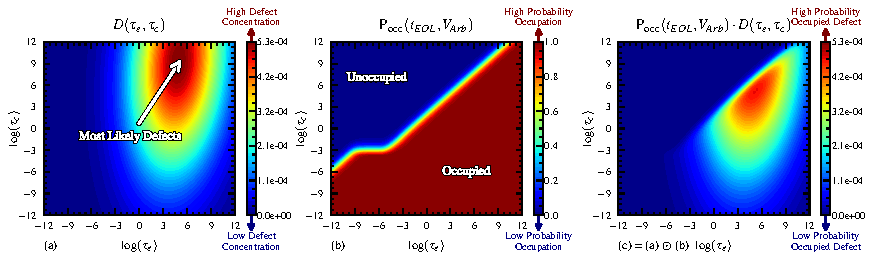
\includegraphics[width=\textwidth,trim={0 0.5mm 0 0mm},clip]{images/ch2/plot_pocc_ddefect_together.pdf}
    \caption{Representations in a logarithmic scale for the time constants of: (a) the distribution of defects used in this work; (b) the probability of a defect being occupied after an arbitrary waveform $V_{Arb}(t)$ with occupied and unoccupied defects highlighted; and (c) the product of both, which provides in the mean degradation through eq. (\ref{Equation:MeanVt}).}
    \label{fig:PDO_Intro}
\end{figure*}
Thus, any defect will have a certain probability of occupation ($\text{P}_{\text{occ}}$) that depends on the history of the operating conditions of the transistor, with a captured carrier adding its specific amplitude to the overall threshold voltage degradation value. Adding together the mean contribution of these defects, the mean degradation $(\overline{\Delta V_\text{th}})$ of a transistor at EOL ($t_\text{EOL}$) when compared to a fresh device (at $t_\text{fresh}$) can be obtained through the PDO model as:
\begin{equation}
\label{Equation:MeanVt}
\overline{\Delta V_{t h}}\left(t_\text{EOL}\right)=\bar{N} \bar{\eta} \iint_0^{\infty} D\left(\tau_e, \tau_c\right)  \Delta \text{P}_{\text{occ}}\left( t_\text{EOL}\right) \mathrm{d} \tau_e \mathrm{~d} \tau_c
\end{equation}
where $\bar{N}$ is the mean number of defects, $ \bar{\eta} $ is the mean change in threshold voltage for a single defect being charged and $\Delta \text{P}_{\text{occ}}\left(t_\text{EOL}\right)$ is the change in probability of occupation at EOL, defined as $\Delta \text{P}_{\text{occ}}\left( t_\text{EOL}\right) = \text{P}_{\text{occ}}\left(t_\text{EOL}\right) - \text{P}_{\text{occ}}\left(t_\text{fresh}\right)$. The value of $\text{P}_{\text{occ}}$ at any point in time depends on the time constants as well as on the biasing history of the transistor and can be expressed in differential form as a differential equation \cite{saraza-canflancaDeterminationTimeConstant2022} whose solution yields a general expression for the probability of occupation after a certain time interval $\Delta t =t_f - t_0$, under constant operating conditions (i.e., bias voltage and temperature) and given an initial value $\text{P}_{\text{occ}}(t_0)$ :
\begin{equation}
\label{Equation:Pocc}
\text{P}_{\text{occ}}(\Delta t)=\frac{\tau_e}{\tau_e+\tau_c}+\left(\text{P}_{\text{occ}}(t_0)-\frac{\tau_e}{\tau_e+\tau_c}\right) e^{-\left(\frac{1}{\tau_e}+\frac{1}{\tau_c}\right) \Delta t}
\end{equation}

An example of the resulting $\text{P}_{\text{occ}}$ from an arbitrary waveform is shown in Fig. \ref{fig:PDO_Intro}(b), as well as the product of this $\text{P}_{\text{occ}}$ with the distribution $D\left(\tau_e, \tau_c\right)$ in Fig. \ref{fig:PDO_Intro}(c), which after applying eq. (\ref{Equation:MeanVt}), results in the mean degradation of the transistor. 

Calculating the mean degradation at EOL requires knowing $\text{P}_{\text{occ}}(t_\text{EOL})$, which implies reevaluating eq. (\ref{Equation:Pocc}) for all CET values each time the operating conditions of the transistor change due to the dependence of ${\tau_e},{\tau_c}$ on temperature and voltage bias. The bias workload $V(t)$ for a transistor can use a \textit{Digital} format, i.e., with two discrete valid voltage values $V_{\text{high}}$ and $V_{\text{low}}$ or an \textit{Analog} format with continuous voltage values. The \textit{Digital} format is simpler, but some information is lost compared to the \textit{Analog} format, as in reality the voltage waveform is not perfectly square, with transition slopes, overshoots, and transient states due to the stacking effect \cite{HongStacking2007, firouziLinearProgrammingApproach2011}. Taking these effects into account has an impact on the resulting mean degradation, for example, not considering voltage overshoots results in an underestimation of 4 \% in degradation, as reported in \cite{gieringNBTIModelingAnalog2014}. 

Although the focus so far has been on obtaining the mean degradation and it will be used in this work as a metric to evaluate the accuracy of the aging prediction, one of the key features of a defect-centric model is the ability to model the aging variability of BTI. This can be done by considering, for each transistor, multiple sets of defects with their specific time constants and amplitude. Then, the contribution of these individual defects to the threshold voltage depending on their $\text{P}_{\text{occ}}$ is added together and multiple aging variability samples of $\Delta V_\text{th}({t_\text{EOL}})$ can be generated for the same transistor. This is crucial to analyze the effect of aging variability at the circuit level \cite{santana-andreoImpactBTIHCI2022,toro-friasFastAccurateReliability2015,vansantenModelingMitigatingTimeDependent2019}, which has been confirmed to have a significant effect on the performance of aged circuits \cite{santana-andreoReliabilityImprovementSRAM2024a, santana-andreoCharacterizingAgingDegradation2022, saraza-canflancaSmartSRAMCellArray2022}. To mitigate the effect of aging in digital circuits, a guardband (i.e., a timing slack on top of circuit delay) is typically used. When no aging variability information is available, a pessimistic, worst-case degradation is uniformly applied to all transistors. Meanwhile, in \cite{vansantenModelingMitigatingTimeDependent2019} it is shown how, by building aging variability-aware cell libraries, the required timing guardband is reduced by 46\%. Consequently, having the ability to consider the aging variability of BTI (i.e., by not abstracting away the defects) is a critical feature of a methodology making aging predictions for large digital circuits. 

In any case, computing $\text{P}_{\text{occ}}(t_\text{EOL})$ considering the complete workload of each transistor until EOL is not feasible: considering a single transistor, an EOL of 10 years (around \num{3.15e+8} seconds) and a complex waveform with a mean frequency of around 4 GHz (in the order of the frequency of commercial processors \cite{AMDRyzenProcessors}) will require approximately \num{2.52e+18} iterations of eq. (\ref{Equation:Pocc}). This is a general problem for defect-centric models and not specific to the PDO model, as calculating the probability of occupation, which depends on the bias history of the transistor, to obtain the final degradation is a common element of defect-centric models \cite{grasserParadigmShiftUnderstanding2011, reisingerUnderstandingModelingAC2011, kaczerDefectcentricPerspectiveDevice2015}. To solve this issue, a naive approach is to assume that the transistor is at a constant, uniform high value (e.g., ignoring aging recovery entirely) so that eq. (\ref{Equation:Pocc}) is only computed once until EOL. However, this is not acceptable, as it significantly overestimates aging \cite{vansantenModelingMitigatingTimeDependent2019}. 
A better approach is to consider that the complex waveform that represents the transistor workload can be modeled as a shorter, representative periodic waveform of duration $\Delta t_{\text{signal}}$, such as the waveform corresponding to an application periodically triggered throughout the lifetime of the circuit. This imposes a limitation on the applications that can be considered, although they are typical in embedded systems \cite{amrouchConnectingPhysicalApplication2015} such as wireless body sensor networks \cite{duchAnalysisFunctionalErrors2020}, and for non-periodic applications the workload size can be adapted to make it more representative. Considering a period of total duration $\Delta t_\text{signal}$ consisting of $n$ total distinct points of bias $V_i$, each $i$-th point with their own $\tau_{ei}(V_i)$, $\tau_{ci}(V_i)$ and $\Delta t_i$ values, a general expression for $\text{P}_{\text{occ}}$ after $\Delta t_\text{signal}$ can be obtained by applying eq. (\ref{Equation:Pocc}) successively: 
% \begin{equation}
% \label{Equation:One_period}
% \text{P}_{\text{occ}}(t_0+ \Delta t_{\text{signal}})=A +B \text{P}_{\text{occ}}(t_0)
% \end{equation}
% where $A$ and $B$ are multiplicative factors:
% \begin{multline*}
% A=\sum_{i=1}^n \frac{\tau_{e i}}{\tau_{e i}+\tau_{c i}} \cdot\left(\prod_{j=0}^{n-i-1} e^{-\left(\frac{1}{\tau_{e(n-j)}}+\frac{1}{\tau_{c(n-j)}}\right)\Delta t_{(n-j)}}\right) \cdot
% \\\left(1-e^{-\left(\frac{1}{\tau_{e i}}+\frac{1}{\tau_{c i}}\right) \Delta t_i}\right) 
% \end{multline*}
\begin{equation}
\label{Equation:One_period}
\text{P}_{\text{occ}}(\Delta t_{\text{signal}})=A +B \text{P}_{\text{occ}}(t_0)
\end{equation}
where $A$ and $B$ are multiplicative factors. Factor $B$ is the weight of the initial probability of occupation on the final value, while $A$ is associated with the shift in probability of occupation due to the applied workload. As $\Delta t$ becomes larger, $A$ dominates over $B$ for more pairs of time constant values. They are defined as:

\begin{equation*}
f_k = e^{-\left(\frac{1}{\tau_{e k}}+\frac{1}{\tau_{c k}}\right) \Delta t_k} \ \ \ \  ; \ \ \ \ B=\prod_{i=1}^n f_i 
\end{equation*}
\begin{equation*}
A=\sum_{i=1}^n \frac{\tau_{e i}}{\tau_{e i}+\tau_{c i}} \cdot \left(1-f_{i}\right) \cdot\left(\prod_{j=0}^{n-i-1} f_{n-j}\right)  
\end{equation*}

Applying eq. (\ref{Equation:One_period}) over successive $M$ periods results in a geometric series, which can be expressed as:
\begin{equation}
\label{Equation:Pocc_periodic}
\text{P}_{\text{occ}}(M \Delta t_\text{signal})=A \frac{1-B^M}{1-B}+B^M \text{P}_{\text{occ}}(t_0)
\end{equation}
 This equation, applicable to any arbitrary periodic waveform \cite{gieringNBTIModelingAnalog2014}, reduces the number of evaluations of eq. (\ref{Equation:Pocc}) from each bias change until EOL to only changes in the considerably shorter representative waveform of duration $\Delta t_\text{signal}$ by considering $M=t_\text{EOL} / \Delta t_{\text{signal}} $. If, say, we assumed a 1 ms workload of an application execution to be representative of the operation until EOL, for the previous example of a mean frequency of 4 GHz the number of iterations of eq. (\ref{Equation:Pocc}) required to estimate degradation at EOL are significantly reduced from \num{2.52e+18} to \num{8e6}. Although the improvement is notable, reducing the number of iterations by 12 orders of magnitude, \num{8e6} iterations per transistor is still too large for a circuit with many transistors.  


\section{Related Work}
\label{section:RelatedWork}
Different approaches have been used to solve the issue of bringing workload-dependent aging predictions to large digital circuits. In \cite{klemmeMachineLearningCircuit2021,klemmeScalableMachineLearning2022a,klemmeEfficientLearningStrategies2022} the calculation of the probability of occupation is circumvented using a curve that translates the average duty cycle of the transistor workload directly into mean degradation, making the problem computationally trivial. Although the curve itself is obtained through a physics-based model \cite{thirunavukkarasuDeviceCircuitFramework2019}, the transistor-level information
$\text{P}_{\text{occ}}(t_0 + t_\text{EOL})$ required to model aging variability is lost in the process. Additionally, only average long-term degradation is obtained, so short-term degradation cannot be properly modeled. 

By contrast, the strategies in \cite{vansantenDesigningGuardbandsInstantaneous2016,AtomisticPseudoRodopoulos2014,fornaciariHarnessingPerformanceVariability2019, duchAnalysisFunctionalErrors2020, amrouchConnectingPhysicalApplication2015} focus on workload compression to obtain the degradation at EOL. Through compression, calculating $\text{P}_{\text{occ}}(t_\text{EOL})$ becomes computationally feasible, and the transistor-level information is not lost. In \cite{vansantenDesigningGuardbandsInstantaneous2016}, a compression technique was introduced that will be referred to as \textit{longest continuous stress (\textit{LCS}) compression}. By calculating the duty cycle $\lambda$ (ON-/OFF-ratio) and the longest continuous ON-time $t_{\text{LCS}}$, the original waveform is reduced to three points, a \textit{stress} phase where high voltage is applied for a time $t_{s}=\lambda t_\text{EOL}$, a recovery phase where low voltage is applied for $t_{r}=(1-\lambda) t_\text{EOL}$ and finally a LCS phase where high voltage is applied for $t_\text{LCS}$, as shown in Fig. \ref{fig:sect2waveformRepresentations}. The driving idea for this compression method is to use the first two phases to represent the average long-term impact of BTI, which is considered frequency independent, and the last LCS phase as a worst-case value of short-term BTI. This approach requires only three iterations of eq. (\ref{Equation:Pocc}) per transistor, significantly reducing the execution time.

\begin{figure}[!b]
    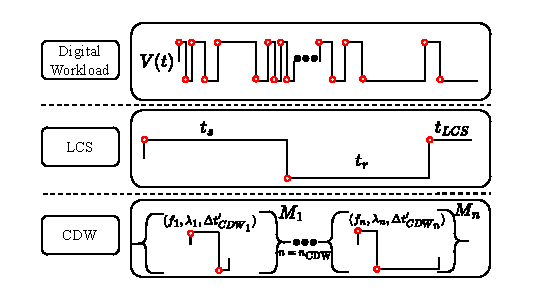
\includegraphics[width=0.48\textwidth,trim={7mm 3.5mm 10.5mm 3mm},clip]{images/ch2/WaveformRepresentationsSect2.pdf}
    \caption{Conceptual waveform representations for state-of-the-art compression techniques. For the \textit{LCS compression}, $t_s$ is the stress phase, $t_r$ the recovery phase and $t_{\text{LCS}}$ the longest continous ON-time in the original workload. For the \textit{CDW compression}, the duty cycle $\lambda$, frequency $f$, and total elapsed time $\Delta t'_{\text{CDW}}$ are the triplet of values that represent one workload segment and $M$ the number of times that segment is repeated. The number of data points, in red, drive the computational effort to obtain the transistor's degradation.}
    \label{fig:sect2waveformRepresentations}
\end{figure}

On the other hand, the authors in \cite{AtomisticPseudoRodopoulos2014} propose taking the uncompressed workload of duration $\Delta t_\text{signal}$, dividing it into segments, and simplifying them into \textit{Compact Digital Waveform} (CDW) segments. This method is termed \textit{CDW compression}, and is further utilized in \cite{duchAnalysisFunctionalErrors2020, fornaciariHarnessingPerformanceVariability2019}. A CDW segment consists on three values: duty cycle $\lambda$, average frequency $f$, and segment duration $\Delta t_{\text{CDW}}$. The values of each CDW segment match the average values of their corresponding original workload segment. In this way, a complex segment that, in the original workload, required many points to be described is reduced to a repeating two-point AC waveform with matching duty cycle and frequency. The number of periods $M$ for each segment is computed as $\Delta t_{\text{CDW}} \cdot f$. The CDW equivalent for the first and last segments of an example workload with their different triplet of values is shown in Fig. \ref{fig:sect2waveformRepresentations}. Thanks to this simplification, $\text{P}_{\text{occ}}$ can be computed significantly faster through eq. (\ref{Equation:Pocc_periodic}). The number of segments $n_\text{CDW}$ used to divide the workload is the user's choice, which introduces a trade-off between accuracy and computation time. Two options are possible when computing the CDW workload \cite{fornaciariHarnessingPerformanceVariability2019}: (a) to employ a fixed number of segments and divide the original workload into a number of intervals of certain, uniform duration $\Delta t_{\text{CDW}}$, or (b) to group segments with similar duty cycle $\lambda$ and average frequency $f$ through a dedicated algorithm.  Through this procedure, the degradation caused by one execution of the representative workload, after $\Delta t_\text{signal}$, can be easily calculated. Still, this degradation must be extrapolated to EOL, a much larger time value (e.g., years) than $\Delta t_\text{signal}$ (e.g., seconds). To perform this extrapolation, the authors in \cite{AtomisticPseudoRodopoulos2014} increase the $\Delta t_{\text{CDW}}$ value of each segment by a proportional factor to cover the entire time range, so that $(\sum{\Delta t'_{\text{CDW}}}) =  t_\text{EOL}$ \cite{AtomisticPseudoRodopoulos2014, fornaciariHarnessingPerformanceVariability2019}. However, this gives \textit{disproportionally more weight to the last CDW segments when determining the final degradation}, causing a prediction error.

 %An algorithm is also proposed as an alternative to group regions with similar CDW values together to improve the trade-off. 

Finally, there are works \cite{gholveCARATReliabilityAnalysis2023,vansantenBTIHCDDegradation2020,gensslerModelingPredictingTransistor2023, amrouchConnectingPhysicalApplication2015, duchAnalysisFunctionalErrors2020} where a ``short" initial aging simulation is performed, obtaining a degradation curve from which the degradation at EOL is extrapolated through a fitting procedure. Some of these fitting approaches employ compression \cite{amrouchConnectingPhysicalApplication2015, duchAnalysisFunctionalErrors2020} to be able to perform longer initial simulations and improve fit quality. However, this approach comes with fundamental drawbacks. By construction, these works abstract defects away, losing the transistor-level information required to accurately consider aging variability. Additionally, a fitting procedure is required for \textit{each individual transistor} in the circuit, adding significant computational and implementation overhead. Furthermore, the length required for the initial simulation to obtain a precise extrapolation is not clear (\qty{1}{\micro s} workload in \cite{gholveCARATReliabilityAnalysis2023,vansantenBTIHCDDegradation2020,gensslerModelingPredictingTransistor2023}, \qty{100}{s} workload in \cite{amrouchConnectingPhysicalApplication2015} and a \qty{10}{min} workload in \cite{duchAnalysisFunctionalErrors2020}) a so-called ``short" simulation can still include a high number of points. Due to these drawbacks, this work will only employ techniques to obtain degradation at EOL \textit{without abstracting defects away}, namely \textit{LCS compression} and the original \textit{CDW compression}. The two techniques proposed in this work (\textit{Gate-level} and \textit{Super CDW} compression, section \ref{section:new_compression}), satisfy this requirement with minimal accuracy loss. 

%Specifically, the works \cite{gholveCARATReliabilityAnalysis2023,vansantenBTIHCDDegradation2020,gensslerModelingPredictingTransistor2023} obtain the degradation curve after a \qty{1}{\micro s} workload. This degradation is extrapolated to EOL by using the easy-to-compute degradation from a DC stress to EOL as reference. In \cite{amrouchConnectingPhysicalApplication2015} the workload is divided into segments, compressing each one into a single two-point waveform that maintains the duty cycle of the original segment but disregards its frequency. Through this procedure, the degradation curve of a 100-s-long workload is obtained, to which the EOL extrapolation is applied. Lastly, in \cite{duchAnalysisFunctionalErrors2020}, they start from a 2 s workload, obtain the CDW-equivalent of that workload, and compute the degradation curve resulting from repeating those 2 s of activity for 10 minutes. Then, they extrapolate to EOL through a fitted curve and perform another short simulation adding the EOL degradation value to capture the short-term degradation.

\section{Reliability Framework}

\label{section:Framework}
In this section, the reliability framework employed in this work and its features are introduced. This framework needs to be able to, from a realistic, representative workload, extract its compressed counterparts and compare the degradation obtained through them with the one obtained without compression.

\subsection{CASE: A circuit-level aging simulator}

To evaluate the aging degradation of each digital gate, we employ our circuit-level aging simulator, CASE \cite{martin-lloretCASEReliabilitySimulation2017}. CASE works with a certain circuit netlist as input, simulates the circuit topology with the SPICE circuit simulator taking into account aging variability and returns the aging-induced degradation per transistor and the circuit's aged performances. This is necessary as current commercial tools such as RelXpert \cite{CadenceReliability} or PrimeSim MOSRA \cite{SynopsysReliability} employ deterministic compact models, unable to accurately model aging variability when compared to defect-centric models. To estimate the impact of aging on digital circuit delays, it is important to work at the transistor level, since not taking individual transistor degradations into account will result in erroneous estimations \cite{khanBTIImpactLogical2012, vansantenModelingMitigatingTimeDependent2019, vansantenNewWorstcaseTiming2019}, with degradation on certain transistors having a larger impact on circuit delay and therefore being more susceptible to aging \cite{mohamedGraphAttentionNetworks2024}. CASE was conceived to study the circuit degradation at the electrical level, obtaining the workload of each transistor through SPICE simulations by specifying a transient simulation. Additional features were required for this work, such as a module to compute the probability of occupation through an efficient implementation of eq. (\ref{Equation:Pocc_periodic}) and the ability to work with workloads expressed in different formats, as detailed in the next subsection. 

%When employing an analog format, a set of gate inputs is specified in a SPICE standard VEC digital vector file format, a transient simulation is performed, and the transistor's workload is obtained. For the digital format, the individual workloads of each transistor are fed directly into the simulator's aging calculation through an external file, bypassing the need to perform electrical simulations in SPICE.


% Given how the number of iterations of (\ref{Equation:Pocc}) is determined by the number of transient points used to describe these analog waveforms, it is important to reduce the number of points employed to describe it to the minimum required. This is distinct from compression, as it refers only to optimizing the workload waveform without changing its shape. For an analog representation, the waveform is represented by evenly spaced points in the time domain printed by the electrical simulator, even if there is no significant voltage change between two points, which is the case for most of the period of a transistor workload in a digital gate. To remove these redundant points, sections of similar voltage values, i.e., where points are within a certain range from the first point of the section, are grouped together. In this work a value of 10 mV is used as the maximum distance between points for each group. However, digital workloads do not require any post-processing, as there are only two possible voltage values. In that case,

% \subsection{Probability of occupation at time zero}
% To apply eq. \ref{Equation:Pocc}, a value for $\text{P}_{\text{occ}}(t_0)$ at time zero is required. Applying that equation for a situation where the device is left unbiased indefinitely $(V = 0, \Delta t = \infty)$, a reasonable assumption for a fresh, unused device, results in a certain, non-zero probability of occupation $\text{P}_{\text{occ}}(t_{0})$ as shown in Fig. \ref{fig:IntialPocc}. One may consider that probability at the begining of the lifetime of a device to be zero, but that would result in a number of defects being occupied on the first application of (\ref{Equation:Pocc}) and a significant mean degradation even after an infinitesimally small $\Delta t$. To correct for the resulting offset, probability of occupation is redefined as:
% \begin{equation}
% \label{Equation:Pocc_adjusted}
% \Delta \text{P}_{\text{occ}}(\Delta t)=\text{P}_{\text{occ}}(\Delta t) - \text{P}_{\text{occ}}(t_0)
% \end{equation}
% Which, for the arbitrary waveform employed in Fig. \ref{fig:PDO_Intro} (b) results in the probability of occupation shown in Fig. \ref{fig:IntialPocc} (b).
% \begin{figure*}[!t]
%     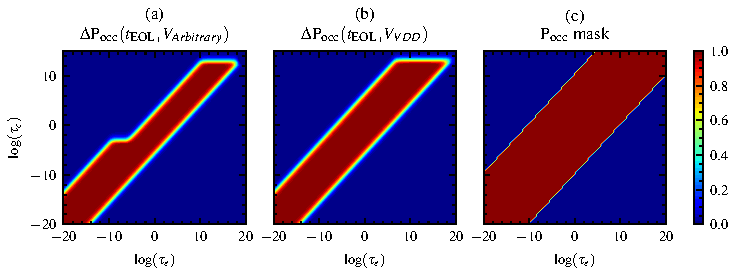
\includegraphics[width=\textwidth,trim={-5mm 0.5mm -5mm 0mm}]{images/ch2/plot_together_pocc.pdf}
%     \caption{Increase in probability of occupation due to the application until EOL of (a) the arbitrary waveform employed in Fig. \ref{fig:PDO_Intro} and (b) the worst-case probability of occupation after constant DC stress. In (c), the mask extracted from (b) of relevant values to calculate with a tolerance of $10^{-6}$, which reduces the computational effort to obtain the probability of occupation without impacting the precision of the degradation prediction.}
%     \label{fig:IntialPocc}
% \end{figure*}
% \subsection{Probability of occupation masking}

% As already mentioned, calculating $\Delta P_{\text{occ}}$ is the critical aspect in terms of execution time to obtain the degradation at EOL. Taking, for example, the arbitrary waveform used to obtain Fig. \ref{fig:PDO_Intro} (b), the change $\Delta P_{\text{occ}}$ is shown in Fig. \ref{fig:IntialPocc} (a).
% To reduce the computational effort to calculate $\Delta\text{P}_{\text{occ}}$ to a minimum, one can determine the region of CET values that is relevant for BTI degradation, so that only the values contained in that area are re-evaluated. A high bound for degradation, considering the gate bias dependence, is a situation in which the transistor remains biased at a high voltage until EOL, equivalent to a constant DC stress. The evaluation of the degradation in this case is trivial, as it requires only one application of (\ref{Equation:Pocc}). The resulting $\text{P}_{\text{occ}}$ is shown in Fig. \ref{fig:IntialPocc} (b). Then, we can define a certain tolerance beyond which the change in the probability of occupation is considered to be zero and not recalculated each time. The mask generated from this approach is shown in Fig. \ref{fig:IntialPocc} (c) and significantly reduces the number of values that must be computed, resulting in an improvement of the execution speed.


\begin{figure}[!b]
    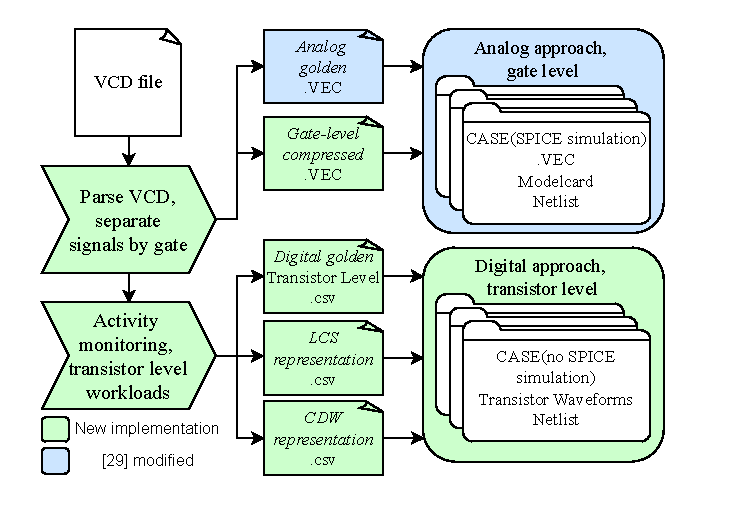
\includegraphics[width=0.48\textwidth,trim={7mm 3.5mm 13mm 4.5mm},clip]{images/ch2/FrameworkCellweaver.pdf}
    \caption{Overview of the flow employed in this work to analyze different compression approaches.}
    \label{fig:Framework Diagram}
\end{figure}
\subsection{Extending CASE to large digital circuits}
\label{ss:ExtendingCASE}
 A custom script is employed to implement the flow illustrated in Fig. \ref{fig:Framework Diagram}, building a reliability framework to extend CASE from small circuits like individual cells to large scale circuits with thousands of cells. First, to obtain the input vectors of each digital cell, a gate-level HDL simulation is performed on the circuit under study, resulting in a standard \textit{Value Change Dump} (VCD) file with input vectors (i.e., cell inputs) expressed in terms of logic levels, that is, $V_{\text{high}}$ or $V_{\text{low}}$ voltage levels. Input vectors are usually automatically translated into individual transistor level waveforms through the SPICE-level transistor topology from the standard cell library from the Process Design Kit (PDK) \cite{vansantenDesigningGuardbandsInstantaneous2016, duchAnalysisFunctionalErrors2020, fornaciariHarnessingPerformanceVariability2019}, in what is referred to as \textit{Activity Monitoring}. This results in a digital format workload of each transistor, which can be fed directly into the aging simulation through an external file without performing SPICE simulations, as shown in the bottom half of Fig. \ref{fig:Framework Diagram}. However, a reduction to a square-wave signal with only two possible logic values purposely removes information (e.g., rise time, transient states in intermediate nodes) potentially altering the predicted aging-induced degradation, particularly in complex cells with many transistors. For example, for two serially connected transistors, the intermediate node can be in an indeterminate state when both transistors are OFF. This state depends on the previous logic state and the charge leakage of that node \cite{zhangAgingAwareGateLevelModeling2021}, a level of detail which cannot be captured by \textit{Activity Monitoring}. An alternative to avoid this is to specify the input vectors in a SPICE standard VEC digital vector file format, perform a transient simulation, and obtain the transistor’s analog format workload. To compare both approaches, we name the uncompressed analog waveform as \textit{Analog Golden} and the uncompressed digital waveform as \textit{Digital Golden}. Later we will introduce other analog/digital compressions and use the golden references as the baseline. Although accurate, these workloads require long execution times that are \textit{unbounded}, i.e., they will require more time for longer workloads.

\subsection{Strategy for low frequency workloads}


\label{subsection:Defect_distribution_shifting}

Performing the aging simulations for a workload corresponding to low switching frequencies introduces an issue, as simulation has to cover at least one full period (which gets longer at the lower frequency) of the representative workload. Unfortunately, the switching frequency is much lower than the clock frequency in a circuit. For instance, an Adder which solely adds small numbers will keep its most significant bit at ``0''. Therefore, the switching frequency $f_\text{switch}$ of a transistor is typically much lower than the clock frequency $f_\text{clk}$ of a circuit. The work in \cite{vansantenWorkloadDependenceSelfHeating2020} showed how in a processor with a 2-GHz $f_\text{clk}$, $f_\text{switch}$ is actually in the kHz-range. These kHz frequencies are currently not supported due to how slower workloads will require more simulation time. An example is shown in Table \ref{tab:lowfreqexample}, where the degradation of an inverter is calculated using the \textit{Analog Golden} approach. It is clear how the simulation time and resulting VEC file size grow linearly with the reduction in frequency, making detailed simulations for slower signals unfeasible. Changing the frequency of the input signal without changing the workload duration is not an acceptable solution either, as it will distort the workload of each transistor.

\begin{table}[!t]
    \caption{Computational effort for low frequency workloads}
    \begin{center}
    \addtolength{\tabcolsep}{-0.2em}
       \begin{tabular}{@{}lcccc@{}}\toprule
        & \multicolumn{3}{c}{Frequency} \\   \cmidrule(lr){2-5}
                        & 500 MHz  & 50 MHz & 5 MHz & $<$1 MHz\\ \midrule
        Waveform Length & \qty{1}{\micro s} & \qty{10}{\micro s} & \qty{100}{\micro s} & Unfeasible \\
        Waveform File Size & 10 MB & 100 MB & 1 GB & Unfeasible\\
        Execution time  & 10 s & 30 s & \makecell{Memory error} & Unfeasible  \\ \bottomrule
    \end{tabular}     
    \end{center}
    \label{tab:lowfreqexample}
\end{table} 

A useful strategy to solve this problem is to keep the workload at a high frequency and instead scale the distribution of defects, changing its time constants to match the reduction in circuit frequency. In this way, only the PDO parameters have to be changed, bypassing the need to change the simulated workload and the slower execution times for slower workloads. \textit{It is important to note that these two approaches are mathematically equivalent and thus result in exactly the same result (no accuracy loss).} This equivalence is proven as follows: we start with a certain \textit{frequency factor} $\epsilon$, which determines how much the workload is slowed down and plug it in eq. (\ref{Equation:Pocc}). If we consider a certain slower workload, $\Delta t$ is increased so that the new $\Delta t' = \epsilon \Delta t$. The technique used is to keep $\Delta t$ unchanged and instead modify the time constants so that $\tau_e', \tau_c' = \tau_e / \epsilon , \tau_c / \epsilon$. Plugging these time constants into eq. (\ref{Equation:Pocc}) results in the \textit{same probability of occupation as the one obtained with the longer $\Delta t$.} The shift in the defect distribution means that we also have to shift the simulation time ($t_\text{EOL}$) in the opposite direction to ensure equivalency when extrapolating through eq. (\ref{Equation:Pocc_periodic}), so that $t'_\text{EOL} = t_\text{EOL} / \epsilon$. 


\section{Proposed compression methods}
\label{section:new_compression}
In this section, we propose two novel compression methods, \textit{Gate-level compression} and \textit{Super CDW compression}.

\subsection{Gate-level compression}
Since the compression methods found in the literature are used only for digital formats of the transistor $V(t)$ waveform, an alternative method is proposed for analog formats. This method is termed \textit{Gate-level compression}. Instead of compressing transistor waveforms, our method compresses the cell's input vectors. For example, consider a 2-input gate with inputs A, B and for which the four possible input vectors are (A = 0, B = 0), (A = 1, B = 0), (A = 0, B = 1), (A = 1, B = 1). The occurrence of each input vector and how frequently they change is recorded for a representative period. We then create a set of synthetic compressed input vectors with each combination appearing only once and maintaining the occurrence ratio of each combination, as shown in Fig. \ref{fig:GateLevelCompression}. The gate is simulated in SPICE for the compressed VEC file generated (as shown in Fig. \ref{fig:Framework Diagram}), extracting the individual transistor waveforms $V(t)$ in analog format. Compared to the methods found in the literature, using this format has the advantage of enabling multiple transistor bias values, while keeping the execution time bounded. This will result in more accurate results as the real bias conditions of the cell are considered (with slopes, overshoots...) and it can be useful in situations where the circuit operates at different supply voltages; for example, a digital circuit that operates between low-power mode ($V_\text{DD}= \qty{0.7}{V}$) and high-performance mode ($V_\text{DD}=\qty{1.0}{V}$) and switches between these two voltages. The drawbacks are requiring more points than a digital signal and performing SPICE calls for short simulations, as well as the inability to properly model short-term BTI, which will come to light in subsection \ref{subsection:freq_dependence}. 

\begin{figure}[!t]
\captionsetup{labelfont={color=blue}}
    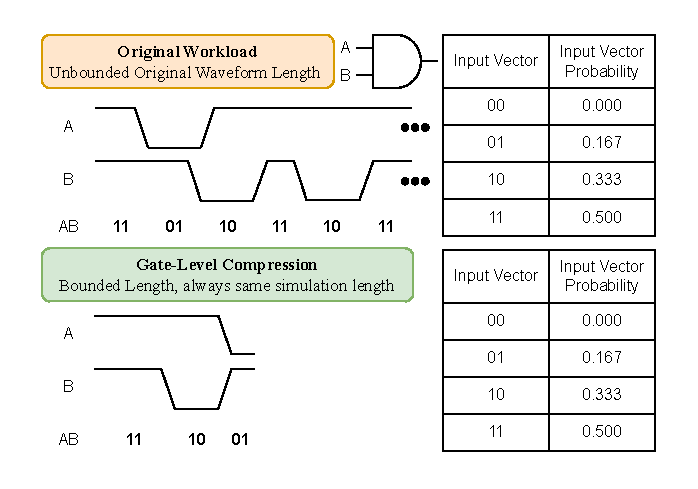
\includegraphics[width=0.48\textwidth,trim={7mm 5mm 7mm 6mm},clip]{images/ch2/GateLevelCompression.pdf}
    \caption{Example showing how \textit{Gate-level} compression is performed on a 2-input AND gate for one period of the representative waveform. }
    \label{fig:GateLevelCompression}
\end{figure}


\subsection{Super CDW compression}
\label{subsection:SuperCDWcompression}
Although the \textit{CDW compression} technique is quite efficient, performing the extrapolation to EOL by increasing the $\Delta t_{\text{CDW}}$ of each segment is a weakness, as it will give significantly more weight to the last CDW segments, resulting in an erroneous prediction. To avoid this weakness, we propose a technique termed \textit{Super CDW compression}. Each waveform is first translated to a set of CDW segments, as in the original \textit{CDW compression}. Then, instead of modifying $\Delta t_{\text{CDW}}$, we repeat the process used to derive eq. (\ref{Equation:Pocc_periodic}), obtaining the degradation after $M_{\text{super}}$ successive sets of CDW segments. Each CDW segment $k$ has its corresponding values $A_k$ and $B_k$, obtained by the expressions in eq. (\ref{Equation:One_period}). Applying a complete set of these segments for a number of segments $n_{\text{CDW}}$ will result in the following expression according to eq. (\ref{Equation:Pocc_periodic}):

\begin{equation}
\label{Equation:Super_CDW}
\text{P}_{\text{occ}}(\Delta t_{\text{signal}})=A_{\text{super}} +B_{\text{super}} \text{P}_{\text{occ}}(t_0)
\end{equation}
with:
\begin{equation*}
A_{\text{super}}=\sum_{k=1}^{n_{\text{CDW}}} A_k \frac{1-B_k^{M_k}}{1-B_k} \cdot\left(\prod_{l=0}^{n_{\text{CDW}}-k-1} B_{n_{\text{CDW}}-l}^{M_k}\right)  
\end{equation*}

\begin{equation*}
B_{\text{super}}=\prod_{k=0}^{n_{\text{CDW}}} B_k^{M_k}
\end{equation*}
In the same way as before, applying eq. (\ref{Equation:Super_CDW}) over successive $M_{\text{super}}$ periods results in a geometric series, which can be expressed as:
\begin{equation}
\label{Equation:Super_CDW_periodic}
\text{P}_{\text{occ}}(M_{\text{super}} \Delta t_\text{signal})=A_{\text{super}} \frac{1-B_{\text{super}}^{M_{\text{super}}}}{1-B_{\text{super}}}+B_{\text{super}}^{M_{\text{super}}} \text{P}_{\text{occ}}(t_0)
\end{equation}


Consequently, we have $M_k = \Delta {t_{\text{CDW}}}_k / f_k$ for each individual segment $k$ and $M_{\text{super}} = \Delta t_\text{signal} /  t_\text{EOL}$ for the collection of segments to reach EOL. Unlike \cite{AtomisticPseudoRodopoulos2014}, our approach repeats the same complete periodic waveform $M_{\text{super}}$ times instead of distorting the CDW segments to match $ t_\text{EOL}$ and applying only the periodic waveform once. An example showing how a CDW segment is extrapolated with our \textit{Super CDW} technique and the original \textit{CDW} approach in \cite{AtomisticPseudoRodopoulos2014} is shown in Fig. \ref{fig:CDWvsSuperCDW}. The \textit{CDW} method increases the $\Delta t_{\text{CDW}}$ of each segment to reach EOL, which results in a distorted workload, where, in the example shown in the figure, a part of the workload that would only last for 10 ms lasts for 1 year. The \textit{Super CDW} compression avoids this issue by performing the extrapolation in two steps, one for the duration of the segment compared to the workload and another for the entire workload. 

\begin{figure}[!t]
    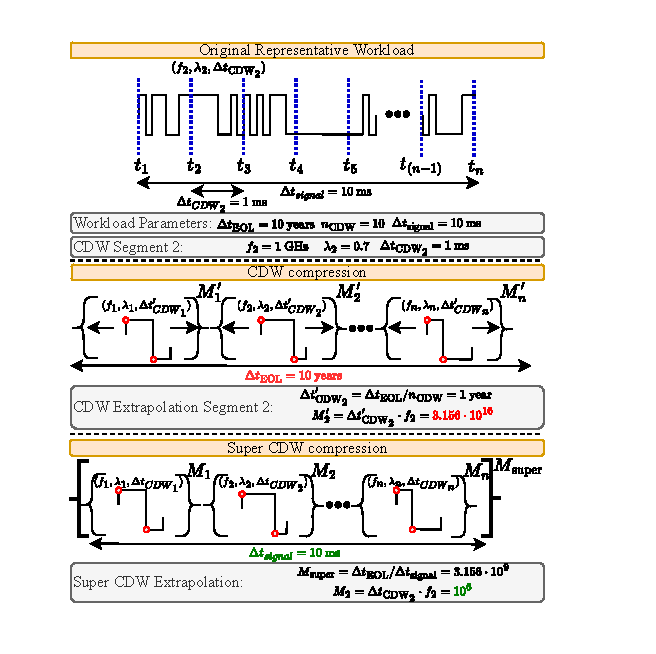
\includegraphics[width=0.48\textwidth,trim={11mm 8mm 18.5mm 5mm},clip]{images/ch2/CDWvsSuperCDW.pdf}
    \caption{Example showing how waveforms are extrapolated to EOL for the \textit{CDW} method \cite{AtomisticPseudoRodopoulos2014} and the \textit{Super CDW} method presented in this work. In this example, the third CDW segment representing 1 ms of an arbitrary workload is used to illustrate the differences between both methods. }
    \label{fig:CDWvsSuperCDW}
\end{figure}

The \textit{CDW} method requires a user-driven trade-off in the number of segments employed. This governs the (super) CDW fidelity/resolution and is a trade-off in accuracy versus computational effort. For instance, we can consider an inverter comprising a PMOS and an NMOS transistor whose input signal has two regions, split in the middle, of complementary signal probability, e.g., $\text{SP } (0.8 = 80\% )$ and $1-\text{SP } (0.2 = 20\%)$, as shown in Fig. \ref{fig:CDWTestPoints}. The length of the signal is set at 10 ms, while the frequency is set at 2 MHz and the degradation is calculated at an EOL of 10 years. The NMOS duty cycle is equal to the signal probability $\lambda_{\text{NMOS}} = \text{SP}$, while the PMOS duty cycle is $\lambda_{\text{PMOS}} = 1 - \text{SP}$. From start to finish the signal in Fig. 6 has a duty cycle of 0.5, however, smaller regions within might temporarily exhibit different duty cycles (shown 0.2 and 0.8 in the signal halves in Fig. \ref{fig:CDWTestPoints}). In fact, if we set $n_\text{CDW}$ to 1, we end up with an overall duty cycle of 0.5 as the later half of the signal averages out with the first half. However, starting from $n_\text{CDW} \geq 2$, we can correctly represent the duty cycle with 0.2 and 0.8 respectively (see Fig. \ref{fig:CDWTestPoints}). Comparing the degradation obtained for two segments for different values of $\text{SP}$ will give an insight into the potential error by oversimplifying the signal. Hence, we can represent the error range as a function of the heterogeneity of the input signal, since the one-segment workload will always predict the same degradation. The difference comes from the finer resolution of the \textit{CDW} method at $n_\text{CDW} > 1$. These temporarily higher or lower duty cycles are taken into account when $n_\text{CDW} > 1$ and might stimulate short-term BTI, i.e., have an impact on the final degradation. Furthermore, the final BTI-induced $\Delta V_{th}$-value differs considerably if the transistor ends under stress (high degradation) or with recovery (low degradation). Since CDW does not determine ending on 0 (OFF = recovery) or 1 (ON = stress), we explore this with the following test: we will consider the difference in the resulting degradation when the last segment is arbitrarily set at high or low and when it is set to finish at the same value as the original signal, i.e., with a matching end state. Exploring the error by setting $n_\text{CDW}$ to 1 (oversimplifying) and 2 (considering temporary differences in each half) is shown in Fig. \ref{fig:CDWTestFinishSweep} (a). We can observe that if the difference between the halves is more extreme (drifting further away from the overall average of 0.5), the importance of using the appropriate number of CDW segments increases. Actual signals might require $n_\text{CDW}$ at values higher than 2, which will increase with the heterogeneity of the uncompressed workload. Using the matching end-state approach results in the best-case error in each case, particularly for these extreme values. Consequently, it will be the approach used moving forward.


\begin{figure}[!t]
    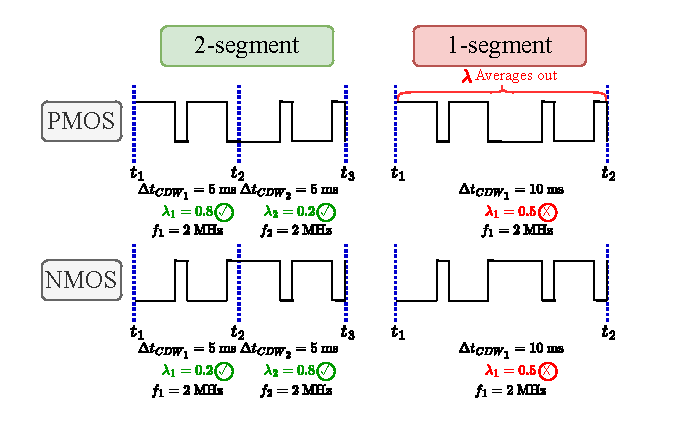
\includegraphics[width=0.48\textwidth,trim={7mm 5mm 13mm 3mm},clip]{images/ch2/CDWTestPoints.pdf}
    \caption{Conceptual representation of the waveforms employed to illustrate the accuracy vs. number of segments trade-off.}
    \label{fig:CDWTestPoints}
\end{figure}
\begin{figure*}[!t]
    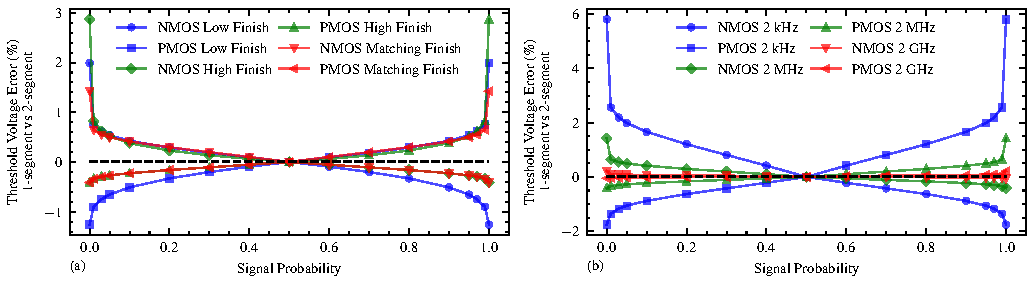
\includegraphics[width=\textwidth,trim={0 0 0 0},clip]{images/ch2/joint_plot_vth_difference_sign_finish.pdf}
    \caption{Error in computing the threshold voltage when comparing the 1-segment to the 2-segment workload as a function of signal probability, with different: (a) finishing values and (b) frequencies.}
    \label{fig:CDWTestFinishSweep}
\end{figure*}


Another aspect that influences this error is the total duration of each segment $\Delta t_{\text{CDW}}$. Depending on the strength of short-term and long-term BTI the error introduced by ignoring the temporarily higher/lower SP becomes higher or lower. This is governed by the switching frequency. To prove this, we repeat the test varying the frequency, as shown in Fig. \ref{fig:CDWTestFinishSweep} (b). We consider 2 GHz, 2 MHz and 2 kHz. The results clearly show how the error increases significantly when considering the slower case, while it is reduced when considering the faster case. Given how the frequency of the signal will determine the significance of the short-term component of BTI, the compression methods used in this work will be tested under different frequencies to ensure they are universally applicable for a wide range of workload frequencies. 




\section{Results and discussion}
\label{section:Results}

In this work, a 32-bit Multiply-and-Accumulate (MAC) unit (a typical computing block in DSPs or in artificial intelligence accelerators such as systolic arrays or tensor processors) is synthesized and used as a benchmark circuit. This block multiplies an 8-bit weight by an 8-bit value and accumulates the result with a 32-bit partial sum. The block contains a total of 459 logic gates, comprising 3,100 transistors. Two workloads are considered for this circuit with the goal of obtaining the degradation after 10 years of operation. For workload ``W1'', we consider $f_\text{clk} = \qty{100}{MHz}$ and inputs (value, weight) follow a uniform random distribution and update every $\qty{10}{ns}$ for a total duration of $\qty{10}{\micro s}$, making it an unbiased, fair workload. This results in an output where the first 16 least significant bits are frequently switching, while the next ones only switch when enough multiplications have been accumulated, as illustrated in Fig. \ref{fig:MAC_bit_dist}. In fact, inspecting the distribution of values, the 16 least significant bits are constantly changing as they are the product of two random numbers. The next bits accumulate the result of the products, so they have a decreasingly low switching frequency. The last bits are zero, as not enough products have been performed to fill the output register. As a result, a wide range of patterns emerge, which will reflect in the internal gate workloads, clearly showing how a certain frequency for the input signal translates into different switching frequencies for the transistors depending on the location within the circuit's netlist. A second workload ``W2'' is considered. It is identical to the previous one for the initial $\qty{8}{\micro s}$ of simulation, but diverges in the final $\qty{2}{\micro s}$, during which all inputs are set to zero and the reset is activated. This represents sleep periods in circuits that, in many applications, are not active during their entire lifetime \cite{duchAnalysisFunctionalErrors2020}. The workload W2 is equivalent to the distribution in Fig. \ref{fig:MAC_bit_dist} for the first 800 product operations and has 0 in all output bits for the remaining 200. While other non-uniform workload scenarios exist, these two serve as unbiased benchmarks: one fully random and the other with a sharp inhomogeneity, facilitating a clear analysis of compression approaches. Simulations are performed with the open-source ASAP7 7nm PDK \cite{vashishthaASAP7PredictiveDesign2017}.
\begin{figure}[!t]
    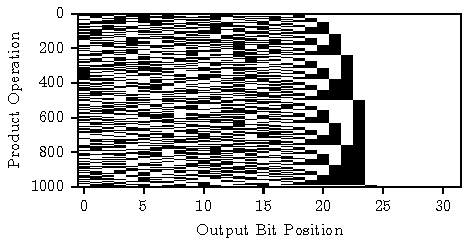
\includegraphics{images/ch2/MAC_bit_distribution.pdf}
    \caption{Output bit value distribution for the first MAC unit testbench, with 0s in white and 1s in black. }
    \label{fig:MAC_bit_dist}
\end{figure}
%with aging parameters extrapolated from experimental measurements \cite{saraza-canflancaDeterminationTimeConstant2022, saraza-canflancaStatisticalCharacterizationTimeDependent2021a}. 
Although the results reported here have been developed for this technology, the methodology is applicable for any technology in which BTI can be properly modeled using individual charge trapping-detrapping events, spanning bulk CMOS (45nm and 65nm in \cite{procelDefectCentricPerspectiveChannel2015} or 28nm in \cite{kaczerDefectcentricPerspectiveDevice2015}), FinFET (8nm and 7nm in \cite{jiangTimeDependentVariability2021a}), Gate-All-Around (GAA) Nanosheet FETs \cite{choudhuryAnalysisBTISHE2020} and stacked Nanowire GAA FETs \cite{chasinBTIReliabilityTimedependent2017}. 

Seven different approaches to obtain the degradation of the MAC unit are considered: two used as reference for accuracy (\textit{Analog Golden}, \textit{Digital Golden}), two from the state-of-the-art  (\textit{5-segment CDW},  \textit{LCS}), two introduced in this work (\textit{Gate-level}, \textit{5-segment Super CDW}) and a baseline \textit{1-segment CDW}. The \textit{1-segment CDW} approach compresses the entire workload into one segment, being the coarsest and fastest implementation of the \textit{CDW} method for which both the \textit{Super CDW} approach proposed in this work and the \textit{CDW} approach in \cite{AtomisticPseudoRodopoulos2014} are mathematically equivalent. However, this represent the crudest approximation of the workload and additional segments are required to obtain higher accuracy in the degradation predictions for non-uniform workloads \cite{AtomisticPseudoRodopoulos2014}. A fixed number of segments is used to compute the \textit{5-segment CDW} and \textit{5-segment Super CDW} workloads, resulting in five segments of equal length. Five segments are the minimum required to properly model the hetereogeneity of the ``W2'' workload, so that the sleep period is included in a single segment. A diagram presenting the workload representation for each approach is shown in Fig. \ref{fig:sect4waveformRepresentations}. For \textit{LCS} and \textit{CDW} the representations were shown in Fig. \ref{fig:sect2waveformRepresentations}. Furthermore, Table \ref{tab:approaches} summarizes the main characteristics of each approach. They are evaluated below in terms of their required computational effort and their ability to predict threshold voltage degradation, analyzing finally how these differences in threshold voltage prediction impact the delay of the digital gates in the circuit.
\begin{figure}[!t]
    
    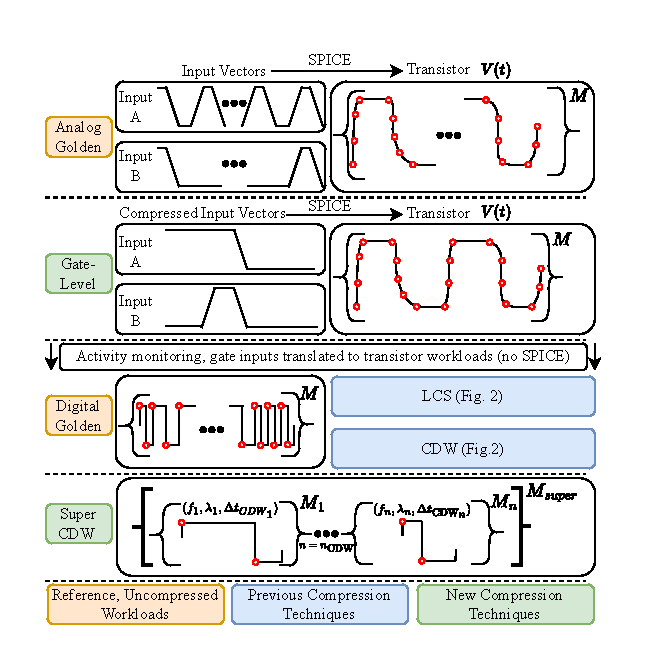
\includegraphics[width=0.48\textwidth,trim={7.5mm 6mm 10mm 8mm},clip]{images/ch2/WaveformRepresentationsSect4.pdf}
    \caption{Conceptual workload representations for the approaches under analysis. Golden workloads are unbounded (will increase in size with larger workloads). }
    \label{fig:sect4waveformRepresentations}
\end{figure}

\begin{table}
    \caption{Compressed and Uncompressed approaches used in this work}
    \begin{center}
    \addtolength{\tabcolsep}{-0.2em}
       \begin{tabular}{@{}lccc@{}}\toprule
        Approach & \makecell{Workload \\ format} & \makecell{ SPICE \\ required} & Eq. (\ref{Equation:Pocc}) iterations \\ \midrule
        \textit{Analog Golden} [Reference] & Analog & Yes & Unbounded (Very high) \\
        \textit{Digital Golden} [Reference] & Digital & No & Unbounded (High) \\
        \textit{Gate-level} [Our work] & Analog & Yes & Bounded (Low)  \\
        \textit{LCS} \cite{vansantenDesigningGuardbandsInstantaneous2016} & Digital & No &  3 \\
        \textit{1-seg. CDW} \cite{AtomisticPseudoRodopoulos2014} & Digital & No &  2 \\
        \textit{5-seg. CDW} \cite{AtomisticPseudoRodopoulos2014} & Digital & No &  10 \\
        \textit{5-seg. Super CDW} [Our work] & Digital & No &  10 \\ \bottomrule
    \end{tabular}     
    \end{center}
    \label{tab:approaches}
\end{table} 

\subsection{Execution speed}
The reduction in execution time through compression is shown in Fig. \ref{fig:Execution time} for workload W1. We plot the execution time of each circuit (cell) versus the number of transistors within the cell to indicate that larger circuits require longer times. Both golden simulations are unbounded and hence impose limits on the maximum circuit/workload size still feasible to simulate. The \textit{Gate-level} approach, although bounded, is considerably slower than the other compressed methods, which do not use an analog representation or require SPICE executions. The compressed methods using a digital format can handle larger circuits in computation times below 1 second. The total computation time of the 1-segment approach is lower by 1.27X when compared to the 5-segment. Execution times are strongly correlated with the number of iterations of eq. \ref{Equation:Pocc} required, as can be seen in Table \ref{tab:approaches}. Note that workloads compressed through the \textit{LCS}, \textit{CDW} and \textit{Super CDW} compression methods have their number of points (and thus, iterations) set to a specific value by construction. The number of iterations in the golden approaches is unbounded because the longer the workload duration, the higher the number of points. The number of iterations of the \textit{Gate-level} approach is bounded because independently of the workload duration, the number of input vectors of each cell is necessarily limited. Except for very short workloads, this number will be considerably smaller than for the golden approaches.

\begin{figure}[!t]
    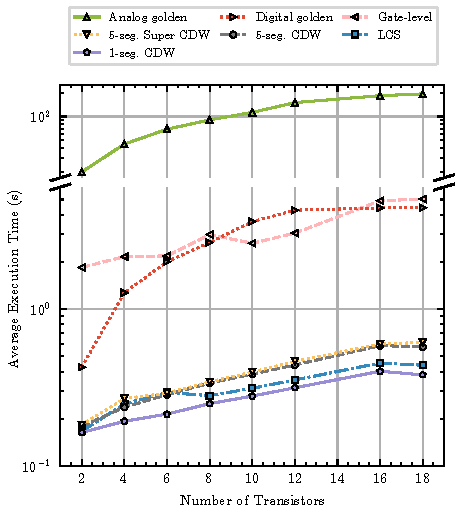
\includegraphics[width=0.48\textwidth,trim={0 1mm 0 1mm},clip]{images/ch2/execution_time_report_plot.pdf}
    \caption{Mean execution time for each approach plotted against the number of transistors for the circuit gates. Segment is abbreviated as seg.}
    \label{fig:Execution time}
\end{figure}

\subsection{Accuracy of Aging-Induced Degradation}
On the other hand, the accuracy of each approach is shown in Fig. \ref{fig:Mean error}, where the mean threshold voltage degradation prediction of each transistor in the digital circuit is compared to the prediction made by the baseline \textit{Analog Golden} approach, which is assumed to be the most accurate. The threshold voltage degradations are obtained by computing eq. (\ref{Equation:MeanVt}) for the $\text{P}_{\text{occ}}$ resulting from each approach. W2 (with sleep period) is harder to compress and results into higher errors. The \textit{Gate-level} approach outperforms the digital approaches, which are hindered by the accuracy loss from the \textit{Activity Monitoring} step. The \textit{1-segment CDW} and \textit{5-segment Super CDW} have an error similar to the \textit{Digital Golden} approach. The \textit{5-segment CDW} approach is more error-prone due to the distortion required to extend each segment to EOL, specially for workload W2. This is explained by the shape of the waveform in W2, where the last $\qty{2}{\micro s}$ are extended to 2 years following the original approach (see Fig. \ref{fig:CDWvsSuperCDW} again for a detailed example). Assuming that the circuit is under continuous operation for 8 years followed by 2 years in sleep is a completely different degradation scenario than having a circuit which operates for $\qty{8}{\micro s}$ followed by $\qty{2}{\micro s}$ sleep continuously. The 2 years of sleep mode are essentially 2 years of DC stress, with conducting transistors capturing many carriers and non-conducting transistors releasing most of the captured ones. This issue does not exist with the \textit{Super CDW} approach, as the EOL extrapolation is correctly made without modifying the length of each segment and distorting the signal. Finally, the \textit{LCS} approach has a significant error under both scenarios because it fails to predict the long-term BTI caused by complex waveforms. Using two long DC periods to model long-term stress will result in a different set of defects being captured when compared to a complex waveform with quick successions of stress and recovery. 
\begin{figure}[!t]
    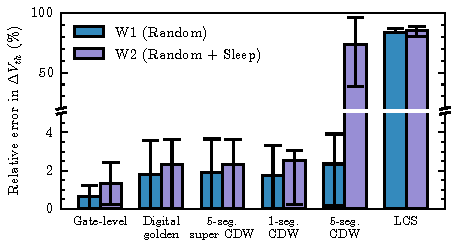
\includegraphics[width=0.48\textwidth,trim={0 1mm 0 0},clip]{images/ch2/mean_error_bar_scatter_report_plot.pdf}
    \caption{Mean relative error with error bars for 10th-quantiles and 90th-quantiles of the considered approaches when predicting the threshold voltage degradation of each transistor after comparing the prediction to the golden analog reference for both workloads under consideration. Transistors with a duty cycle of 0 or 1 are not considered as DC stress requires no compression. }
    \label{fig:Mean error}
\end{figure}
Given how the W2 workload is the hardest to compress accurately for all approaches, it will be the one used moving forward. A closer look into the error in predicting the degradation of each transistor is shown in Fig. \ref{fig:cellwise error}. These results confirm how \textit{Activity Monitoring} is causing the errors for the \textit{Digital Golden} approach in complex cells (those errors above 10 mV) that are harder to translate from input signal to transistor duty cycle, as discussed in subsection \ref{ss:ExtendingCASE}. Meanwhile, transistors corresponding to inverters (i.e., those within a 2-transistor gate) do not have a significant error for the \textit{Digital Golden} approach. The \textit{Activity Monitoring} errors are carried into the \textit{1-segment CDW} and \textit{5-segment Super CDW} predictions, as they employ a digital format for the workload. It is also clear how the \textit{LCS} and \textit{5-segment CDW} approaches fail to accurately represent the degradation of most transistors.

\begin{figure}[!t]
    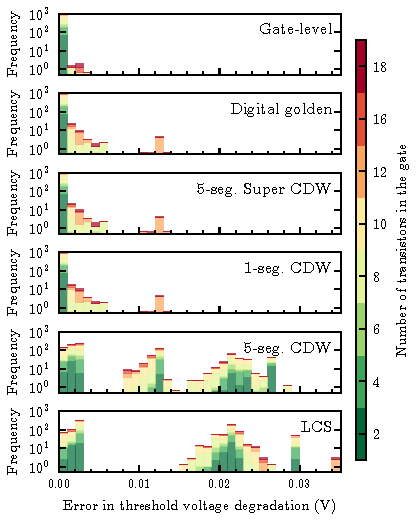
\includegraphics[width=0.48\textwidth,trim={0 0 0 1mm},clip]{images/ch2/absolute_error_histogram_plot.pdf}
    \caption{Error in threshold voltage degradation prediction for each transistor in the circuit using workload W2. The transistors are differentiated depending on the complexity (defined as the number of transistors) of their corresponding gate.}
    \label{fig:cellwise error}
\end{figure}

%In any case, if short-term BTI is a concern, one may add a LCS phase to any of the previous approaches without a significant cost in execution time. 

    % The large error bars are mostly due to outliers caused by transistors with a duty cycle close to 0 or 1, where a small difference in the waveform can result in a large relative difference in degradation.
\subsection{Delay change estimation}

It is important to translate the threshold voltage degradation, which is a transistor-level parameter, into the relevant circuit-level figure of merit for digital standard cells, i.e., propagation delays. A detailed list of the logic gates present in the 32-bit MAC design is shown in Table \ref{table:gates}, ranging in complexity from 2-transistor inverters to 18-transistor 8-input complex cells such as AOI332. A digital gate with more than one input will have more than one valid timing path for a transition propagating from input to output. A change in the output with a certain unateness requires the appropriate, gate-dependent combination of input values (determined by the logic operation of the gate), and the propagation delay will be different depending on the timing path's input and the state of the other inputs. In this way, the number of possible delays increases rapidly with the number of gate inputs, as shown in the second column of Table \ref{table:gates}. 

\begin{table}
	\caption{32-bit MAC gates and their characteristics}
	\begin{center}
		\begin{tabular}{lcccc} \toprule
			Gate & Inputs & Delay combinations & Transistors & Instances \\ \midrule
			INV & 1 & 2 & 2 & 103 \\
			NOR2 & 2 & 4 & 4 & 25 \\
			NAND2 & 2 & 4 & 4 & 62 \\
			XOR2 & 2 & 8 & 10 & 48 \\
			XNOR2 & 2 & 8 & 10 & 66 \\
			NAND3 & 3 & 6 & 6 & 25 \\
			OAI21 & 3 & 10 & 6 & 7 \\
			AOI21 & 3 & 10 & 6 & 4 \\
			AO21 & 3 & 10 & 8 & 2 \\
			NOR4 & 4 & 8 & 8 & 2 \\
			NAND4 & 4 & 8 & 8 & 4 \\
			AND4 & 4 & 8 & 10 & 2 \\
			OAI211 & 4 & 16 & 8 & 1 \\
			A2O1A1I & 4 & 20 & 8 & 40 \\
			OAI31 & 4 & 20 & 8 & 2 \\
			AOI31 & 4 & 20 & 8 & 2 \\
			AOI22 & 4 & 24 & 8 & 8 \\
			OAI22 & 4 & 24 & 8 & 20 \\
			OAI222 & 6 & 108 & 12 & 16 \\
			AOI332 & 8 & 448 & 16 & 13 \\
			OAI332 & 8 & 448 & 16 & 2 \\
			AO332 & 8 & 448 & 18 & 3 \\
			OA332 & 8 & 448 & 18 & 2 \\ \bottomrule
		\end{tabular}
	\end{center}
	\label{table:gates}
\end{table}


\begin{figure}[!t]
    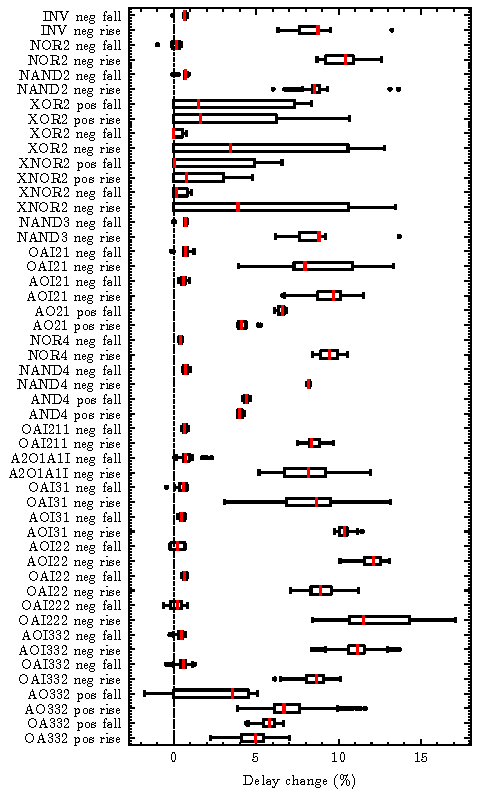
\includegraphics[width=0.48\textwidth,trim={0 0 0 0},clip]{images/ch2/box_cellwise_delay.pdf}
    \caption{Box plot showing the distribution of the mean increases in delay caused by aging degradation, using the \textit{Analog Golden} approach and the W2 workload. }
    \label{fig:cellwisedelay}
\end{figure}

With these considerations in mind, the delay change distributions are shown in Fig. \ref{fig:cellwisedelay}. A distinction is made between rise and fall delays as well as their unateness, which may be positive (0 $\xrightarrow{}$ 1, ``pos'') or negative (1 $\xrightarrow{}$ 0, ``neg''). Not all combinations are possible for all gates by construction. There are also edge cases where only the transistors that oppose the change in output value when a transition occurs are the ones that degrade, resulting in a delay reduction, which explains the small negative values \cite{santana-andreoImpactBTIHCI2022}. Beyond the gate characteristics, degradation is driven, naturally, by the workload that propagates from the MAC inputs to each individual gate. The variety in distributions for each gate in Fig. \ref{fig:cellwisedelay} clearly illustrates why careful and precise transistor-level predictions of degradation are necessary to arrive at the delay increase of each gate. These distributions are for the mean degradation, and the aging variability of each transistor needs to be considered on top of it to obtain a complete aging prediction. 

%An important factor to consider is the fact that BTI degradation in PMOS (Negative Bias Temperature Instability, NBTI) is significantly greater than BTI degradation in NMOS (Positive Bias Temperature Instability, PBTI). This can be clearly distinguished in the aforementioned topologically simpler gates (INV, NAND, NOR ...) where the increase in rise delay, determined mostly by the degradation of the pull-up network (NBTI), is significantly larger than the increase in fall delay, determined mostly by the degradation of the pull-down network (PBTI).

Given these degradation values in terms of the delay obtained for the \textit{Analog Golden} workload, they can be compared to the degradation obtained through each compression method. The resulting error is expressed in terms of percentage points (p.p.). To clarify with an example, given a delay increase of 10\%, if the prediction of the compressed waveform results in an increase of 6\% the error is $-4$ p.p. (40\% less), while if the prediction is of 12\% the error is $2$ p.p. (20\% more). An overestimation (positive p.p.) implies that the gate will not degrade as much as predicted, leading to design overcompensation when specifying the guardband and just an unnecessary performance loss. Meanwhile, an underestimation (negative p.p.) implies that the gate will degrade more than expected, leading to unacceptable timing violations. Hence, slight overestimation is fine, while even minor underestimation is catastrophic. The compression errors are shown in detail in Fig. \ref{fig:delay_compression_error}. The \textit{Gate Level} approach manages the best accuracy, matching the original degradation in most cases. \textit{Digital Golden}, \textit{1-segment CDW} and \textit{5-segment Super CDW} are similar in accuracy, having a higher error than the previous approach, with the \textit{1-segment CDW} method having a slightly larger number of overestimations.  All four of these distributions are reasonably symmetric, not exceeding 3 p.p. of over- or underestimation in any case. The \textit{5-segment CDW} does introduce significant errors in both directions, ranging from $-10$ p.p. of underestimation and 7.5 p.p. of overestimation. Given how the highest degradations observed in Fig. \ref{fig:cellwisedelay} are around 12.5\%, these errors are large. The \textit{LCS} method leads almost exclusively into underestimation, due to the inability to capture long-term degradation by applying the recovery phase. 

\begin{figure}[!t]
    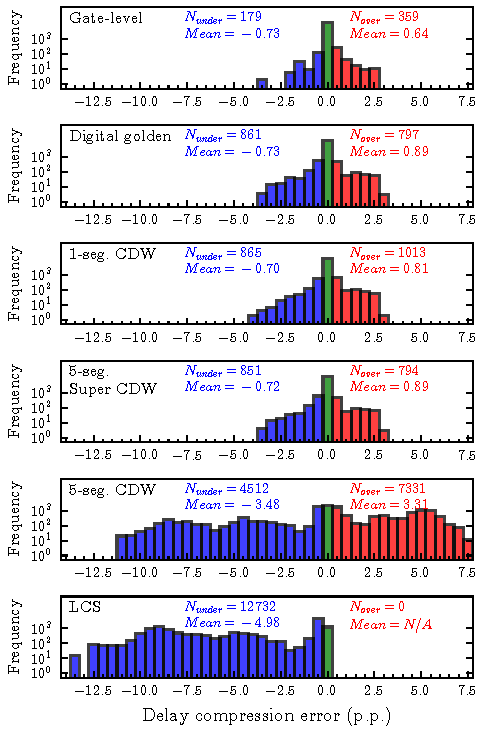
\includegraphics[width=0.48\textwidth,trim={0 0 0 0},clip]{images/ch2/error_delay_report_plot.pdf}
    \caption{Distributions for errors in the delay estimation of each compression method expressed in percentage points for workload W2. Mind the logarithmic scale for the y-axis. Underestimations, which can lead to timing violations, are shown in blue, while overestimations, which can lead to unnecessary performance loses, are shown in red. Those cases where compression matches the original prediction are shown in green.}
    \label{fig:delay_compression_error}
\end{figure}

\subsection{Frequency dependence}
\label{subsection:freq_dependence}
The technique detailed in subsection \ref{subsection:Defect_distribution_shifting} is employed to analyze the performance of each compression method under different frequency scenarios. The short-term component of BTI is driven by the latest bias conditions of the transistor. In low-frequency scenarios, the time transistors are at a high or low bias before switching increases, making the short-term component greater in amplitude, as stress and relaxation times are longer. The time constants are shifted by a certain \textit{frequency factor} (without any loss in accuracy, see subsection \ref{subsection:Defect_distribution_shifting}), which determines the shift in terms of orders of magnitude. For example, applying a \textit{frequency factor} of 3, $f_\text{clk}$ goes from $\qty{100}{MHz}$ to $\qty{100}{kHz}$ and the workload duration goes from $\qty{10}{\micro s}$ to $\qty{10}{ms}$. Frequency factors range from $-1$ to 9, to get a wide range of frequencies from GHzs to $<$ 1 Hz. To evaluate the performance of each compression method, the number of overestimations, underestimations, and mean deviation for each case are used, as in Fig. \ref{fig:delay_compression_error}. 

\begin{figure}[!t]
    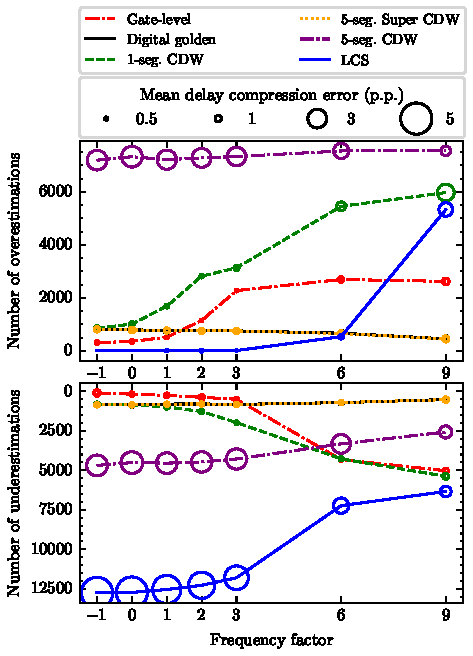
\includegraphics[width=0.48\textwidth,trim={0 0 0 0},clip]{images/ch2/delay_error_frequency_dependence.pdf}
    \caption{Bubble chart indicating the number of over and under estimations in terms of delay prediction from each compression method for a set of different \textit{frequency factors} and workload W2. The bubble size indicates the mean deviation. The \textit{Digital Golden} and \textit{5-segment Super CDW} approaches overlap each other in accuracy.}
    \label{fig:delay_error_frequency_dependence}
\end{figure}
\begin{figure}[!t]
    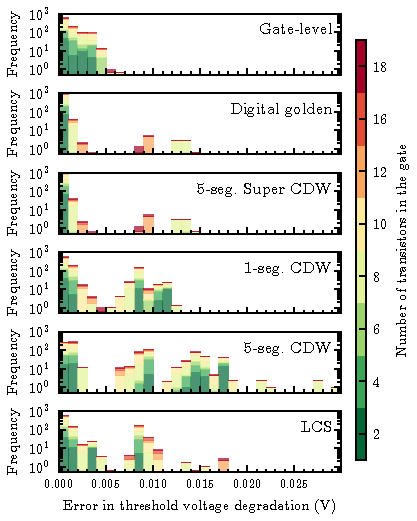
\includegraphics[width=0.46\textwidth,trim={0 0 0 1mm},clip]{images/ch2/absolute_error_histogram_plot_tau6.pdf}
    \caption{Error in threshold voltage degradation prediction for each transistor in the circuit, workload W2 and a \textit{frequency factor} of 6.}
    \label{fig:cellwise error tau6}
\end{figure}
The results are shown in Fig. \ref{fig:delay_error_frequency_dependence}. It is clear that the conclusions extracted from the original workload do not hold for the entire frequency range. \textit{Digital Golden} and \textit{5-segment Super CDW} are able to maintain a consistent error rate, associated with the \textit{Activity Monitoring} step, and which slightly decreases with slower frequency as the importance of that error is reduced when the short-term component becomes stronger. It is remarkable to note that the \textit{5-segment Super CDW} compression is able to exactly match the \textit{Digital Golden} accuracy. Both the \textit{Gate-level} and \textit{1-segment CDW} suffer from the fact that they cannot properly represent the heterogeneity of the signal. Although for high frequencies \textit{Gate-level} is the best in terms of accuracy and \textit{1-segment CDW} matches \textit{Digital Golden} and \textit{5-segment Super CDW}, they start to become inaccurate (over- and underestimations, higher mean error) when frequency decreases. For the \textit{1-segment CDW} this is consistent with the results shown in Fig. \ref{fig:CDWTestFinishSweep} (b) and discussed in Subsection \ref{subsection:SuperCDWcompression}: Increasing the number of CDW segments and correctly representing the heterogeneity of the signal becomes more important as the short-term component of BTI becomes more significant. The \textit{Gate-level} generates a synthetic workload that matches the characteristics of the entire representative workload but is not able to capture the hetereogenity of the signal to model the short-term component properly. Finally, both \textit{5-segment CDW} and \textit{LCS} are not able to accurately represent the degradation for the entire range. These conclusions are further supported by inspecting the error in the threshold voltage degradation for a specific \textit{frequency factor}, as shown in Fig. \ref{fig:cellwise error tau6} for a \textit{frequency factor} of 6. \textit{5-segment Super CDW} and \textit{Digital Golden} have the error associated with \textit{Activity Monitoring} and complex cells, while \textit{Gate-level} and \textit{1-segment CDW} perform significantly worse than with the original frequency. \textit{LCS} performs better when short-term BTI is more dominant, it shifts from underestimation to overestimation as the longest continuous stress time increases at lower frequencies. Overestimation is a built-in feature of \textit{LCS} as it tries to provide the worst-case degradation scenario. It is clear how, when considering which compression method to employ, the frequency of the signal is important. Given that there is no universal switching frequency for a large digital circuit, it is not straightforward to have a clear cut-off point for all instances in the circuit. In that context, the \textit{5-segment Super CDW} is clearly superior and the best general approach given the aforementioned variety in switching frequencies, as it achieves great accuracy and low execution times across the board. However, considering that originally the input signal changes every 10 ns with a $f_\text{clk}$ of 100 MHz and that both the \textit{Gate-level} and \textit{1-segment CDW} approaches become comparatively worse to the \textit{5-segment Super CDW} for a \textit{frequency factor} of 2, we can estimate that, in this specific scenario, for a $f_\text{clk}$ in a range of GHzs to tens of MHzs, using the \textit{Gate-level approach} is best for accuracy, and using a \textit{1-segment CDW} is valid for speed. 





\section{Conclusions}
\label{section:Conclusions}

After a thorough exploration of the compression techniques found in the literature and comparing them on the same workload and circuits for the first time, we have successfully introduced two novel approaches (\textit{Gate-level} and \textit{Super CDW} compression) that surpass existing methods in terms of speed and accuracy. The accuracy of each compression method is not solely evaluated based on the predicted threshold voltage shift per transistor, but additionally also wholistically, i.e., with aging-aware circuit delay estimations. We explored a wide range of conditions (e.g., switching frequencies) to illustrate the robustness of our proposed techniques. For the entire range of frequency values, using the compression methods found in the literature (\textit{CDW} and \textit{LCS}) yields unacceptable results (up to 73.34\% for the \textit{5-segment CDW} average error in threshold voltage and 84.85\% for \textit{LCS}) in terms of accuracy. On the other hand, the proposed \textit{Super CDW} method performs well in the entire frequency range in terms of accuracy and speed. Specifically, it is 295X faster compared to the analog uncompressed workload, 8X faster than the digital uncompressed workload, and has a 2.31\% average error in threshold voltage degradation, matching the digital uncompressed workload, while featuring a low upper bound for execution time and making it the superior choice in most scenarios. For high transistor switching frequencies, \textit{Gate-level} is the best choice in terms of accuracy (1.31\% average error in threshold voltage degradation) and \textit{1-segment CDW} is the best choice in terms of speed (1.27X faster than \textit{5-segment Super CDW)}, but both drop significantly in accuracy as frequency decreases. Hence, only the proposed \textit{Super CDW} technique with an appropriate number of segments has a consistent, low error rate for the entire range of switching frequencies.

%due to their inability to correctly represent the impact of a workload's heterogeneity on the short-term component of BTI.

% In future work, these approaches will be used to predict the long-term degradation of larger digital circuits with a strong foundation in the physics of BTI without compromising speed. 

\chapter{SRAM PUFs}
\label{chap:3}


This chapter presents a more detailed revision of SRAM-PUFs, so that contributions presented in the next chapters can be better understood. This starts by considering the architecture of the standard SRAM array, followed by a description of the 6T cell and a basic overview of its operation. Afterwards, its use as a PUF is evaluated with the advantages and challenges it presents. Finally, the environmental conditions and aging mechanisms that may affect the SRAM PUF's reliability are considered. 

\section{SRAM architecture}

SRAM stands for static random-access memory. It is static since it does not need to be refreshed periodically, the data will be held as long as the memory is powered up, as opposed to a DRAM (dynamic random-access memory). When it powers down, it does lose its data, which makes it a volatile memory. SRAM memory is faster and more expensive than DRAM; it is typically used for CPU cache while DRAM is used for a computer's main memory.

An SRAM memory cache consists of an array of SRAM memory cells along with peripheral circuitry, such as row and column address decoders, sense amplifiers or write drivers \cite{Singh2013}. An SRAM cell is a type of memory that uses a latch to store a bit. The cell is bistable (has two stable states), one corresponds to the value zero and the other to the value one.

Commercial SRAM chips include millions of memory cells distributed in columns and rows, conforming a two dimensional array. For example, a 4 MB SRAM memory will include 4,194,304 memory cells. To illustrate how the array is organized, a simple 4x6 SRAM array, corresponding to 24 bits, is shown in fig. \ref{fig:SRAM_array}. It is illustrative since a commercial SRAM array uses a similar structure, with larger address decoders and arrays. Cells are distributed in rows and columns. All cells in a row share a line, called wordline $(WL)$, that is activated by the row decoder output. Likewise, all cells in a column share a pair of lines, called bitlines $(BL \ \mathrm{ and } \ \overline{BL})$, that are activated by the column decoder output. Encoding the address instead of specifying a row and a column reduces the number of interconnections by a factor of $log_2N$, where $N$ is the number of cells. This is of critical importance to make large SRAM arrays viable.  


\begin{figure}[H]
    \centering
    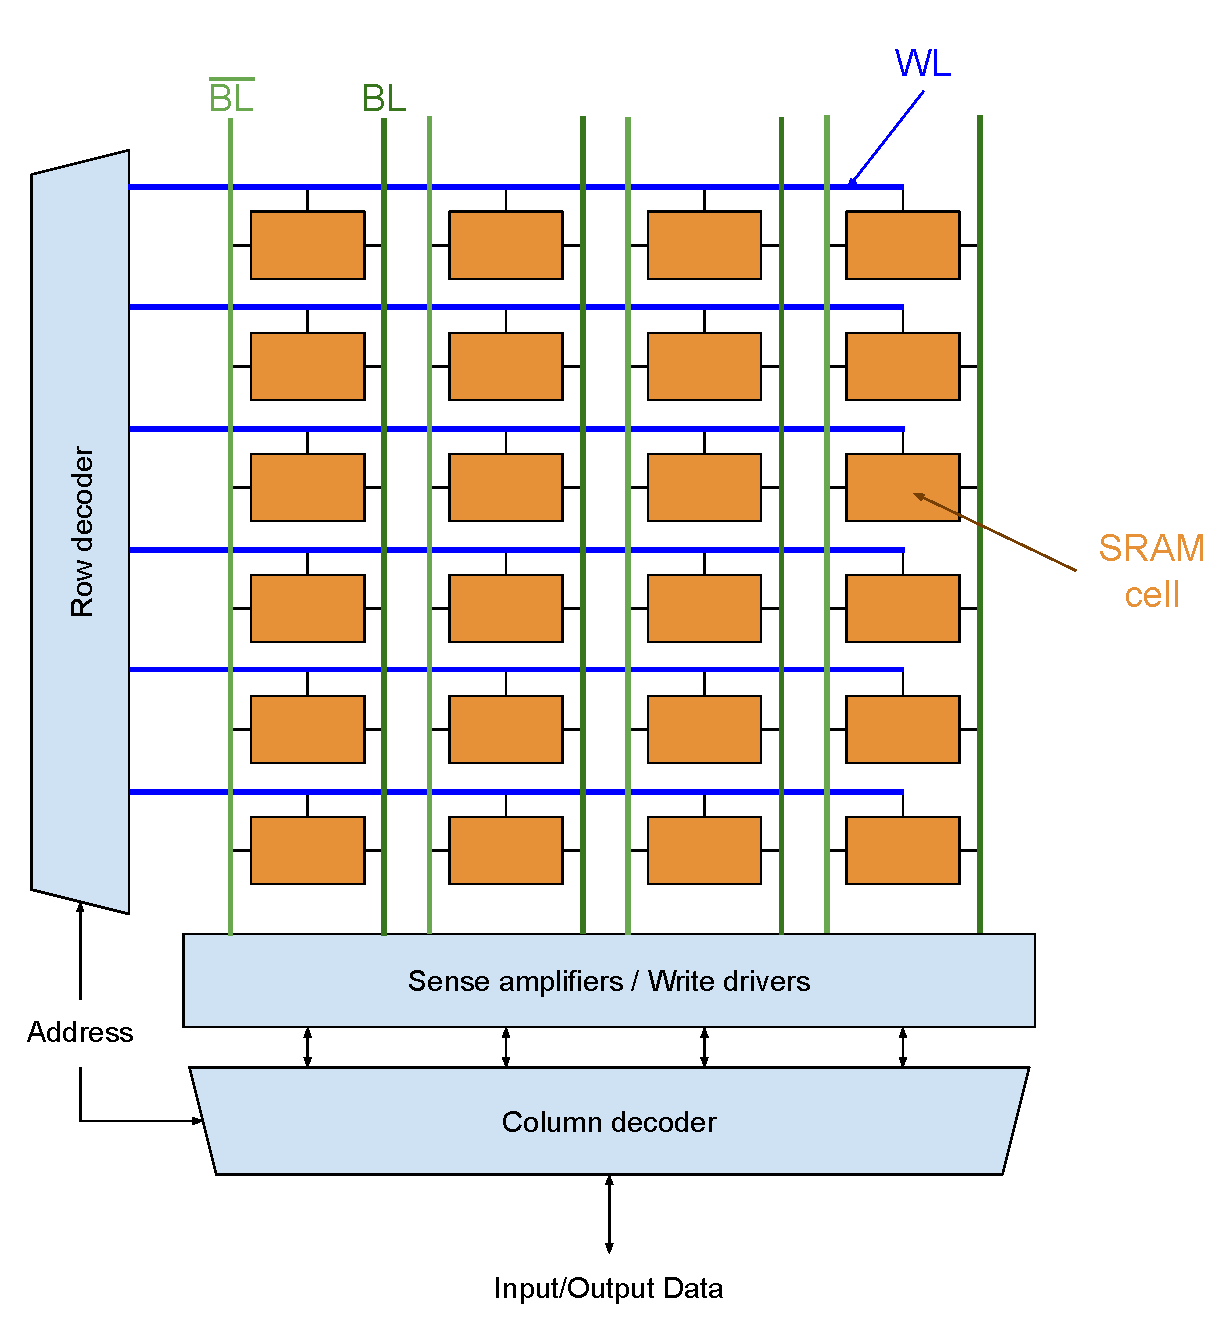
\includegraphics[width=11cm]{images/SRAM Architecture.pdf}
    \caption{A simple 4x6 SRAM array structure}
    \label{fig:SRAM_array}
\end{figure}

 Each individual cell is addressed by selecting the appropriate wordline and bitline pairs. As mentioned before, these ``lines'' are selected by the row decoder and the column decoder, respectively, setting the specified wordline high and connecting the pair of bitlines to the sense amplifiers for reading, or to the write drivers for writing. Sense amplifiers amplify a small differential voltage to a full swing digital output signal, the value of the selected cell. Write drivers control the voltage level during write operation to change the state of the cell to the provided input.  
 
 In the following section the topology of the SRAM 6T cell, which is the one used in this work, will be examined in detail, along with how the read and write operations are performed. 





\section{The SRAM 6T cell}

%More detailed description of SRAM PUFs along with a description of an SRAM cell. 4-5 Páginas


Although other designs exist, the standard topology for the SRAM cell is the 6T cell shown in fig. \ref{fig:SRAM}, which uses six transistors and is the cell generally employed in PUFs. 

\begin{figure}[H]
    \centering
    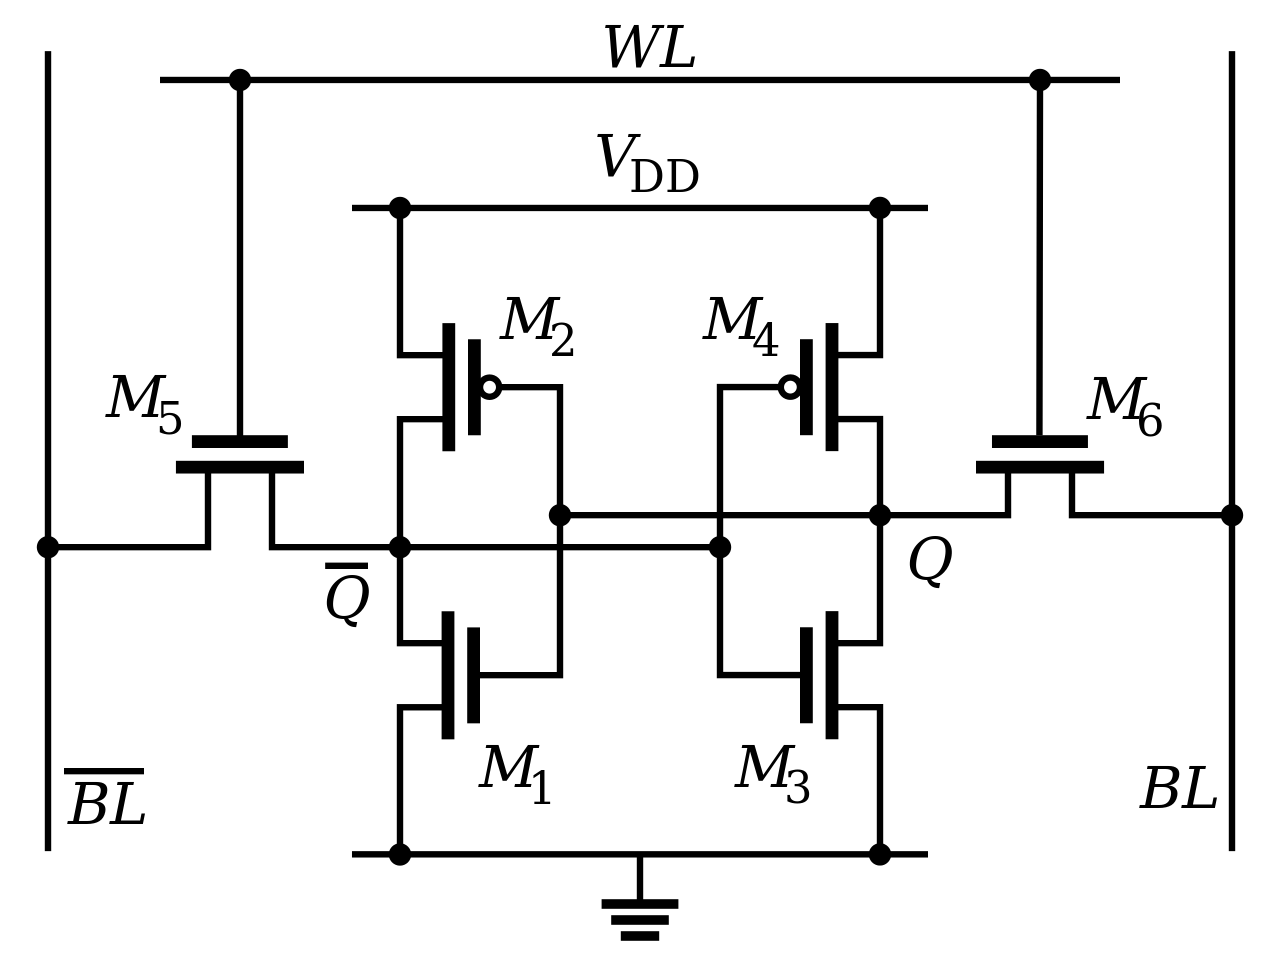
\includegraphics[width=9cm]{images/SRAM_Cell.png}
    \caption{Schematic of a 6T SRAM cell}
    \label{fig:SRAM}
\end{figure}

This cell is comprised of two cross-coupled inverters and two NMOS access transistors. The inverters set the voltage value of the internal nodes of the cell ($Q$ and $\overline{Q}$) through one pull-up (PMOS) and one pull-down (NMOS) transistor each. When the system is in a steady state, one of the nodes is at a high voltage ($V_{DD}$) and the other at a low voltage ($V_{SS}$ or ground). The values corresponding to $V_{DD}$ or $V_{SS}$ depend on the implementation. Accordingly, there are two possible states:

\begin{enumerate}
    \item $Q$ at high voltage and $\overline{Q}$ at low voltage.
    \item $Q$ at low voltage and $\overline{Q}$ at high voltage.
\end{enumerate}

One of the states represents the logic value 1 and the other 0. The choice is arbitrary but must be consistent. Without loss of generality due to the symmetry of the cell, from this point onward logic 1 corresponds to the first state and logic 0 to the second state. Positive feedback forces the cell into one of the two states. The SRAM cell has three modes of operation: holding, writing and reading. The access transistors isolate the cell from the circuit during holding to preserve the written value, and allow access during writing and reading. Access transistors are controlled by the wordline ($WL$) signal. The other connections to the cell are the bit line signals ($BL$ and $\overline{BL}$) which are connected to the internal nodes when the access transistors allow them. The bit line connection affects the internal nodes by introducing a small perturbation. This is useful for changing the state of the cell during the writing operation but must not be strong enough to change the state during the reading operation. These two modes of operation are examined now with more detail. 

\subsection*{Reading}

 To perform the reading, both bit-lines are first driven to the high voltage value, $V_{dd}$. Then, the $WL$ signal is activated. The process is illustrated in fig. \ref{fig:readwrite} (b). One internal node will be at a low voltage and the other at a high voltage. The bitline connected to the node at low voltage discharges slightly, while the other bitline stays at roughly the same voltage. This difference is measured by a sense amplifier. The stored value is determined depending on which one of the bitlines has the higher voltage. 

The internal node at low voltage rises its value as well when connected to the bitline. If this perturbation is small, the cell's feedback will be able to compensate once the reading is over. However, if it reaches a critical value it could alter the stored value and cause an error. The magnitude of this perturbation depends on the relative value between the width of the inverter's pull-down transistor ($M_1$ or $M_3$, depending on the state) and the width of the access transistors ($M_5$ and $M_6$ respectively). 

\begin{figure}[H]
    \centering
    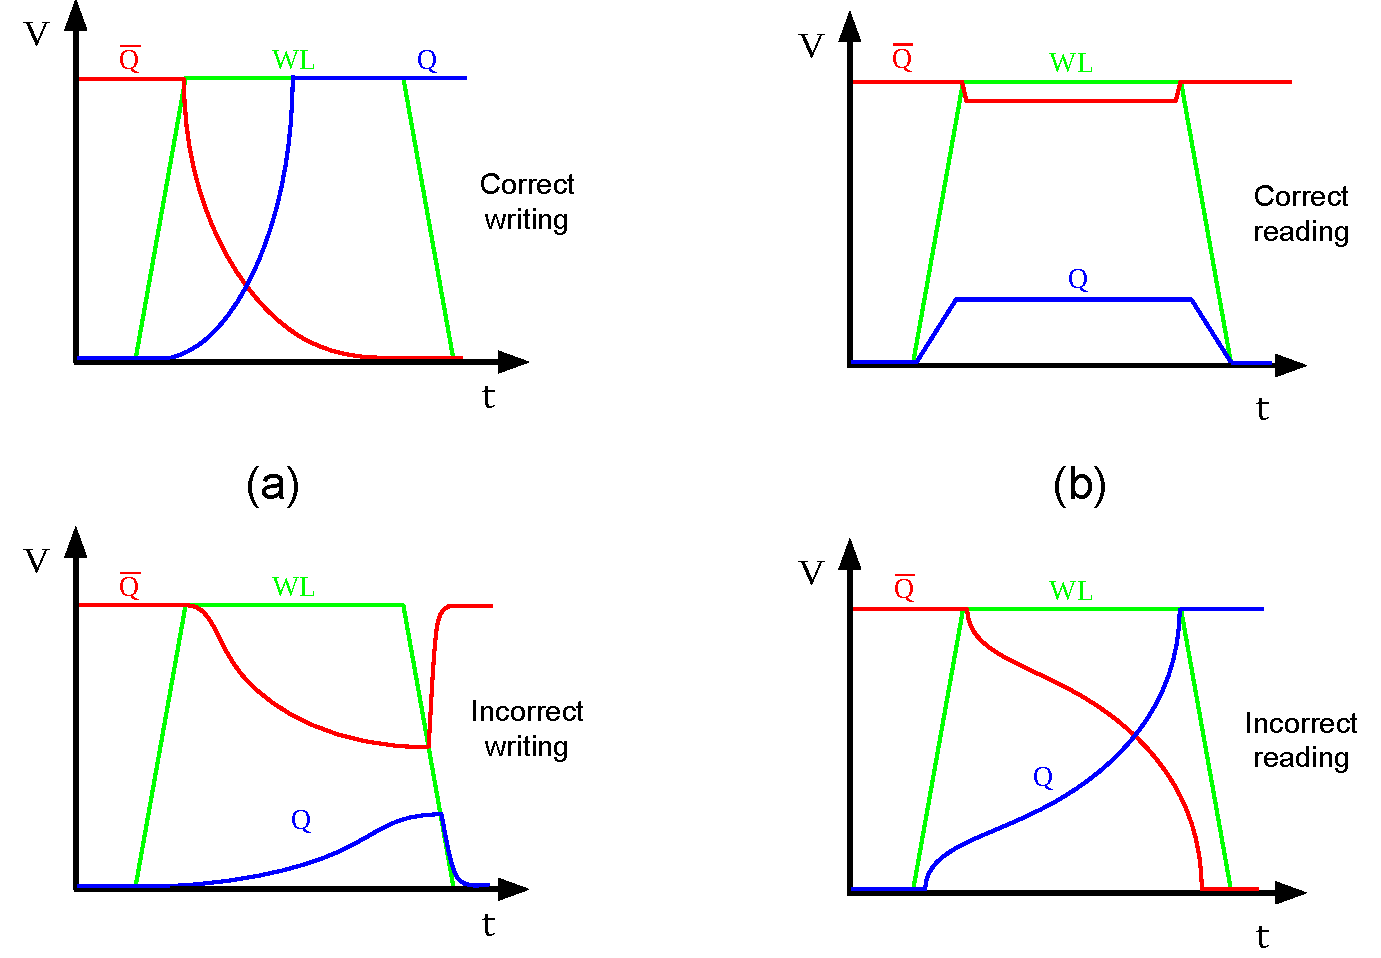
\includegraphics[width=15cm]{images/SRAM Read_Write.pdf}
    \caption{Voltage at the internal nodes and $WL$ signal during a successful and unsuccessful writing (a) and reading (b) operation. The starting state is $Q$ at low voltage and $\overline{Q}$ at high voltage, but the diagram would be similar for the other starting state. }
    \label{fig:readwrite}
\end{figure}

\subsection*{Writing}

This process is illustrated in fig. \ref{fig:readwrite} (b). To perform the writing, each bit-line is driven to the desired voltage values of their respective internal nodes through the write drivers. The objective when writing is to change the state of the cell. To accomplish that, the node at low voltage has to increase to high voltage, and vice versa. The $WL$ signal is then activated. The low voltage node increases its voltage at a rate which depends on the relative widths of the inverter's pull-up transistor ($M_2$ or $M_4$, depending on the state) and the width of the access transistors ($M_5$ and $M_6$ respectively). The high voltage node decreases its voltage at a rate which depends on the relative widths of the inverter's pull-down transistor ($M_1$ or $M_3$) and the width of the access transistors ($M_5$ and $M_6$ respectively). 

If the perturbance is not big enough, the voltage will not be flipped by the time the $WL$ signal is deactivated. In this case, the nodes will go back to their original state and the writing operation will have failed. Accordingly, the widths of the transistors must be tuned to have a perturbation strong enough for writing and weak enough for reading. 




\section{SRAM as a PUF}

An introduction to SRAM PUFs was provided in \ref{ss:cap2SRAM}. Since SRAM PUFs are the focus on this work, a more detailed look into them is required. As explained before, SRAM PUFs exploit the mismatch due to fabrication process variability between the two inverters by measuring the start-up value of SRAM cells, determined by which one of the two inverters powers up faster. 

Whether one inverter or the other powers up faster depends on the threshold voltage $V_{th}$ of the different transistors. In order to simply illustrate this, we will consider that the strength of the cell depends only on the $V_{th}$ values of the PMOS transistors $M_2$ and $M_4$ (using fig. \ref{fig:SRAM} as reference). As an example, suppose that mismatch causes $|V_{th2}|$ to be smaller than $|V_{th4}|$. When the cell powers up, i.e. $V_{dd}$ rises, $M_2$ will start conducting before $M_4$, causing $\overline{Q}$ to go up to high voltage and $Q$ to low voltage, resulting in a power-up state of ``0'' by the criteria defined earlier.   

 Generalizing this example, if the difference between threshold voltages is $\Delta V_{th}=|V_{th2}|-|V_{th4}|$ the cell should power up to ``1'' for $\Delta V_{th}>0$ and to ``0'' for $\Delta V_{th}<0$. However, some cells (below 20\%) with $|V_{th2}|\approx|V_{th4}|$ may change their power-up values when this is determined at different moments, due to operating temperature differences, supply voltage variations, aging or noise \cite{Baturone2015}. These are considered unstable and are largely responsible for the bit flips in the SRAM response. Most cells (above 80\%) have a large enough difference to reliably power-up to the same state and are considered stable.
 
 Figure \ref{fig:celldistribution} illustrates this if the distribution of the transistors' threshold voltage is assumed to be gaussian as in the mismatch models \cite{Hofer2010}. Cells with values in the middle region are considered unstable, shown in red. The bias does not have to be very strong to have a stable cell; so, generally, a majority of cells are considered stable, shown in light green. 

\begin{figure}[t]
    \centering
    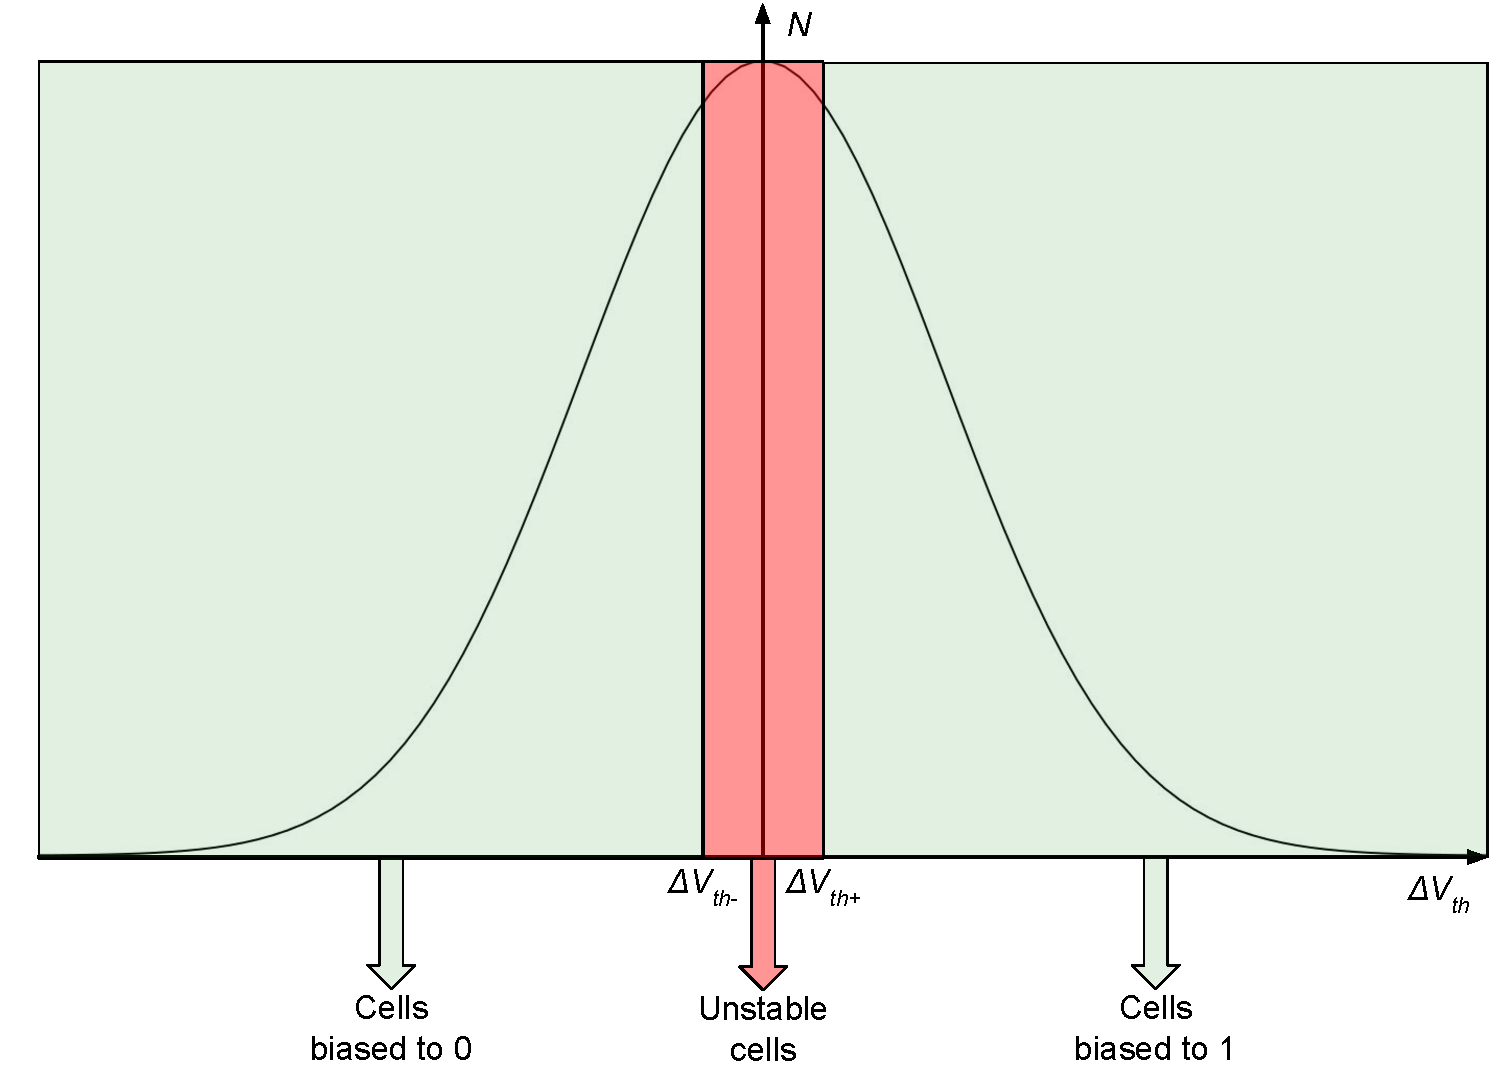
\includegraphics[width=14cm]{images/Cell distribution.pdf}
    \caption{Number of cells $N$ corresponding to a certain value of $\Delta V_{th}$. Cells with $\Delta V_{th} \approx 0 $ are unstable, while those to the left are biased to zero and those to the right to one.}
    \label{fig:celldistribution}
\end{figure}


Although only the mismatch of the PMOS transistors was considered regarding the power-up state of the cell, the mismatch of the NMOS transistors is important as well. The NMOS transistor that starts conducting faster pulls its node to low voltage, as they are connected to $V_{ss}$. Their contribution depends on how fast the SRAM powers up \cite{Wang2018}, i.e. the power supply ramp rate. This contribution ranges from NMOS mismatch having almost no impact for near instant power-ups (1 ns) to NMOS mismatch having the same impact as PMOS for slow power-ups (1 s). In the second case, $\Delta V_{th}$ is calculated as $\Delta V_{th}=|V_{th2}|+|V_{th3}|-|V_{th4}|-|V_{th1}|$. 
In essence, depending on the difference in threshold voltages the cell will have more or less reliability working as a PUF. It is important to keep in mind that the stable cells still have some degree of unreliability over a large enough number of power-ups \cite{Liu2017}.

The standard solution for unstable cells in the context of PUFs used for key generation is employing helper data algorithms, but the requirements of heavy ECCs are quite costly as described in the previous chapter. Some proposed SRAM bit selection techniques which attempt to select only stable cells are evaluated in the next chapter. If the unstable cells are separated from the stable ones, they can still be useful for entropy generation \cite{Baturone2015}. 

Other approaches specific to SRAM PUFs have been studied to reduce this problem \cite{Baturone2015}. For example, in \cite{Okumura2011,Hofer2010,Shifman2018} they use a custom design of the SRAM cell. Specifically, in \cite{Okumura2011} write drivers and PMOS switches are added to the SRAM cell, in \cite{Hofer2010} circuitry to measure the threshold voltage is added so that only stable cells are used and in \cite{Shifman2018} the power supply of each inverter is routed independently to perform small independent variations and select stable cells based on their response to those variations and a Miller capacitor is added to increase stability. However, these methods are costly and renounce to one of the main advantages of SRAM PUFs, the ability to use generic SRAM cells already present in ICs. 

\section{Sources of reliability degradation}

It is important as well to characterize how local temperature differences, supply voltage variations and aging affect PUF reliability. An overview is provided in the following subsections. From this understanding the reliability of the SRAM PUF can be properly measured and new techniques to boost reliability can be developed and tested.

 
\subsection{Supply voltage}


SRAM cells power up by rising their supply voltage from zero to $V_{dd}$. There are two different aspects concerning supply voltage and reliability.

On the one hand, possible deviations from the nominal value of supply voltage $V_{dd}$. This is usually tested by evaluating the circuit at supply voltages of $\pm 10 \%$ of the nominal supply voltage \cite{Schrijen2012}. However, the start-up value of the cell should be established during power-up and the supply level at the end of the ramp should not have a large impact on SRAM PUF reliability.

On the other hand, the ramp-up time has a pronounced effect on reliability \cite{Claes2012,Wang2018}. There is a wide range to choose from, from the order of $\mu s$ to around one second. The issue is that faster ramps are better for high temperatures while slower ramps are better for low temperatures \cite{Cortez2013}. According to this, in \cite{Cortez2013} a proposal to dynamically change the ramp-up time is made. In any case, the effects vary according to the device design and a careful choice based on experimental data must be made to achieve optimal reliability. 


\subsection{Temperature}

Temperature is quite influential on the performance of ICs. In SRAM PUFs it directly affects the characteristics of transistors, and, therefore, the PUF response \cite{Schrijen2012}. Accordingly, it is of great importance to properly characterize its effects for reliability. This is done by measuring the behaviour of the chip in a certain temperature range. These ranges depend on the implementation. Although the specific range may vary, generally accepted ones are \cite{operating_temperature}:

\begin{itemize}
    \item Commercial: $0\degree \mathrm{C}$ to $70\degree \mathrm{C}$
    \item Industrial: $-40\degree \mathrm{C}$ to $85\degree \mathrm{C}$
    \item Military: $-55\degree \mathrm{C}$ to $125\degree \mathrm{C}$
\end{itemize}

Usually, PUFs are tested in the industrial range \cite{VanDerLeest2012,Schrijen2012,Cortez2013}. Depending on the SRAM design, the worst case reliability can be in either extreme of the temperature range \cite{Schrijen2012}. 

\subsection{Aging}
\label{sec:aging}
%Causes of aging in SRAM (BTI, HCI, RTN). Models of aging developed. 5-6 páginas

As technology scaling continues in microelectronics, SRAM cells become smaller and time dependent degradation of electrical properties (aging) becomes more severe. Understanding aging is important to predict errors in any electronic implementation. 

%This is employed in \cite{Garg2014,Mispan2016,Bhargava2013}.

Aging can have a wide range of effects, from a change in threshold voltage, and the consequent increase in delay times, to permanent failure. Naturally, the change in threshold voltage is very important in SRAM PUFs since it may change the bias of one cell from one state to another during power-up. Aging depends in more variables than just time, being influenced by workload during operation, environmental conditions and electrical stress. 

%Electrical stress implies supply voltage levels higher than the nominal value of  $V_{dd}$.To accelerate aging a useful and common technique is to apply high electrical stress for short periods of time, trying to emulate a degradation similar to years of operation under nominal conditions \cite{Maes2014}. An SRAM PUF aged this way provides an estimation on the worst case reliability regarding aging. 

 The aging mechanisms generally considered for SRAM cells are Bias Temperature Instability (BTI), Hot-Carrier Injection (HCI), Time-Dependent Dielectric Breakdown (TDDB) and Electromigration (EM) \cite{Kraak2018}. BTI, HCI and TDDB occur in the gate oxides of transistors while EM happens in the interconnect metal lines. BTI and HCI are the main concern regarding PUF reliability as they occur at nominal voltages. More studies have been performed for BTI than HCI but an exact model for either one has not yet been created \cite{Schlunder2012}. In the subsequent subsections the effects of BTI and HCI will be considered qualitatively. 


\subsubsection{BTI}

BTI includes NBTI (Negative-Bias Temperature Instability) effects, which occur in PMOS transistors, and PBTI (Positive-Bias Temperature Instability) effects, which occur in NMOS transistors. NBTI is generally dominant over PBTI for small technology nodes \cite{Kraak2018} and consequently NBTI aging is the main focus of study. NBTI increases the threshold voltage of the transistors and the consequent decrease in drain current and transconductance. It is caused by positive charges built up in the MOS gate insulator due to the application of negative gate bias. There is no consensus on a model for NBTI \cite{Stathis2018}. The Reaction-Diffusion model holds that NBTI is a diffusion-limited process and the Defect-Centric model holds that it is reaction-limited. According to the first one, interface traps are generated during operation and these interface states become positively charged when the PMOS device is biased in the "on" state, i.e. with negative gate voltage. According to the second one, preexisting traps located in the bulk of the dielectric are filled with holes coming from the channel of PMOS.

Either the oxide electric field caused by negative gate voltages or elevated temperatures can produce NBTI, but a stronger and faster effect is produced by their combined action. Due to technology scaling, the magnitude of the electric field becomes greater, so NBTI is always going to be present and will be stronger as scaling keeps progressing \cite{Schroder2003}. This degradation phenomenon reveals a stochastic and discrete nature for technology nodes in the nanometer range, which means that identical transistors (and therefore circuits) may age differently \cite{Kaczer2010}. The effects of NBTI have a permanent and a temporal component, since part of the degradation can be recovered over time when stress is removed (i.e. when the gate voltage is removed). 

%Some of these include guard-banding, gate-sizing and voltage tuning. Differential structures will make the stress less noticeable as well \cite{Lee_aging_techniques}.

How does BTI affect an SRAM cell? The 6-T standard cell shown in fig. \ref{fig:SRAM} is considered. Suppose it is biased so that $Q$ is at the high voltage at power up. This corresponds to a state 1 according to the criteria expressed earlier. Accordingly, the left NMOS transistor has a smaller threshold voltage than its pair and/or the right PMOS transistor has a smaller threshold voltage than its pair. They will be the first to turn ON and will make the cell take the 1 logic value due to the feedback. If node $Q$ is at a high voltage following the nomenclature of fig. \ref{fig:SRAM} the NMOS transistor $M_3$ will be off and the PMOS transistor $M_1$ will be on and suffering PBTI.  On the other hand, node $Q$ will be at a low voltage, so PMOS transistor $M_4$ will be off and the NMOS transistor $M_2$ will be on and suffering PBTI. NBTI occurs in the PMOS transistor, so this transistor will be more affected. In any case, threshold voltage increases over time, consequently reducing the initial bias of the cell. The reasoning is the same if the cell is biased towards 0. If the cell is written to its non preferred value, BTI will instead increase the existing bias. 

If the initial power-up bias of a cell is reduced over time, stable cells will turn unstable progressively. However, it can be solved by storing the non preferred value in the cell, which mitigates the stress caused during functional operation. This technique, called directed accelerated aging (DAA) \cite{Roelke2018}, can be used to increase the initial bias and the resulting reliability of the cell. It can even be used to flip the initial skew of a cell and make it strongly biased to the other state. This is used in \cite{Garg2014} to improve the uniformity of the PUF response as well. 

%In \cite{Maes2012} a SRAM PUF is shown to have an increase of about 2\% in terms of Bit Error Rate after 4.5 years of operation based on experimental results where accelerated aging was applied. 


\subsubsection{HCI}

HCI is a phenomenon by which the threshold voltage of a transistor is altered when high energy carriers are trapped in the gate oxide, as in BTI. However, HCI is caused by a flowing drain current, in which moving charge carriers (the hot carriers) break up the bonds between silicon and hydrogen at the boundary between the transistor channel and gate dielectric. The carriers need a certain kinetic energy to achieve this. When velocity saturates, electron's average velocity will not increase but the random kinetic energy of some electrons can achieve the required kinetic energy to break the silicon-oxide barrier due to random collisions. Once electrons start to break the barrier, a small leakage current appears and traps can occur.

The requirements for HCI to be present are high electric fields and long mean free path, i.e. the average distance travelled by an electron between collisions. As in BTI effects, technology scaling makes high electric fields common. Increasing the voltage will make degradation more pronounced. On the other hand, the mean free path for electrons to be accelerated is inversely proportional to temperature, so lower temperatures will increase HCI. In digital gates, it occurs only when the device switches, so the effect is proportional to the signal activity factor (ratio of average number of signal transitions to clock transitions and the clock frequency) \cite{Sengupta2017}.  The  recoverable component of HCI degradation is very small compared to BTI \cite{Bhargava2013}, so HCI has high permanence (does not lessen significantly over time).

Although BTI degradation is the most popular for DAA in the literature, in \cite{Bhargava2013} HCI is used to boost reliability by applying stress through a $V_{DS}$ increase. The advantages over BTI are shorter stress time, high permanence and requiring only a one-time reinforcement stress. 

% \subsection{TDDB}



% \subsection{EM}

% Electromigration is the transport of conductive material in the direction of the current caused by the momenta exchange between current carrying electrons and the conductor's metal lattice. The effect is proportional to current density, so miniaturization increases it as well. The main consequence is the eventual loss of connections or failure in a circuit. However, proper design practices consider the effects of electromigration \cite{Lienig2018}. These practices are generally incorporated in the automated design tools. Electromigration has been known and studied for a long time and is relatively predictable, so it isn't a major concern for SRAM PUFs in their usual lifespan.









\chapter{A new method for bit selection in SRAM-PUFs}
\label{chap:4}

A naive approach to SRAM PUFs would be to choose a random selection of cells among the available cells. As pointed out in section \ref{sec:HDAs}, this would leave all the work to the ECC step and would come at a prohibitive cost considering the limited reliability of standard SRAM PUFs responses. There are a variety of criteria to choose the best cells in a SRAM. An ideal selection would improve the reliability of the response without being detrimental to uniqueness or uniformity. These cells should also provide a better response under the worst corners of performance, not just under nominal conditions. 

In this chapter, some commonly used prevalent bit selection techniques are discussed. They serve as reference to compare the new bit selection technique, Maximum Trip Supply Voltage (MTSV), that tries to improve the existing techniques. Afterwards, this new technique is presented and validated with experimental data.

\section{Multiple Evaluation}
\label{sec:ME}
In Multiple Evaluation (ME) several power-up evaluations are performed on each cell, either to elaborate a response by majority vote \cite{Bhargava2012}, or to discard those cells that do not always power-up to a given value \cite{Baturone2015}. A key aspect of this method is that a fixed number of measurements must be selected: for instance, 20 measurements were chosen as a good trade-off in \cite{Baturone2015}. However, it is also shown in \cite{Baturone2015} that many cells that returned the same value for the first 20 power-ups, returned at least one “erroneous” value (i.e., their nonpreferred value) in the next 60 measurements, since 80 power-ups were performed to each cell. This is illustrated in fig. \ref{fig:unstable_me} for one of the chips used later in this work. In \cite{Bhargava2012}, no specific number of evaluations is set; however, the necessity of making this choice is clearly stated and the possibility of using from 10 to 100 evaluations is mentioned. Nevertheless, the appropriate number of evaluations depends on several factors, such as the technology node. Choosing well would thus require a tedious experimental study. In fact, this type of multiple evaluation may require a prohibitively high number of power-ups, thus delaying an on-line response, and significant hardware resources \cite{Liu2017}. 

\begin{figure}[H]
    \centering
    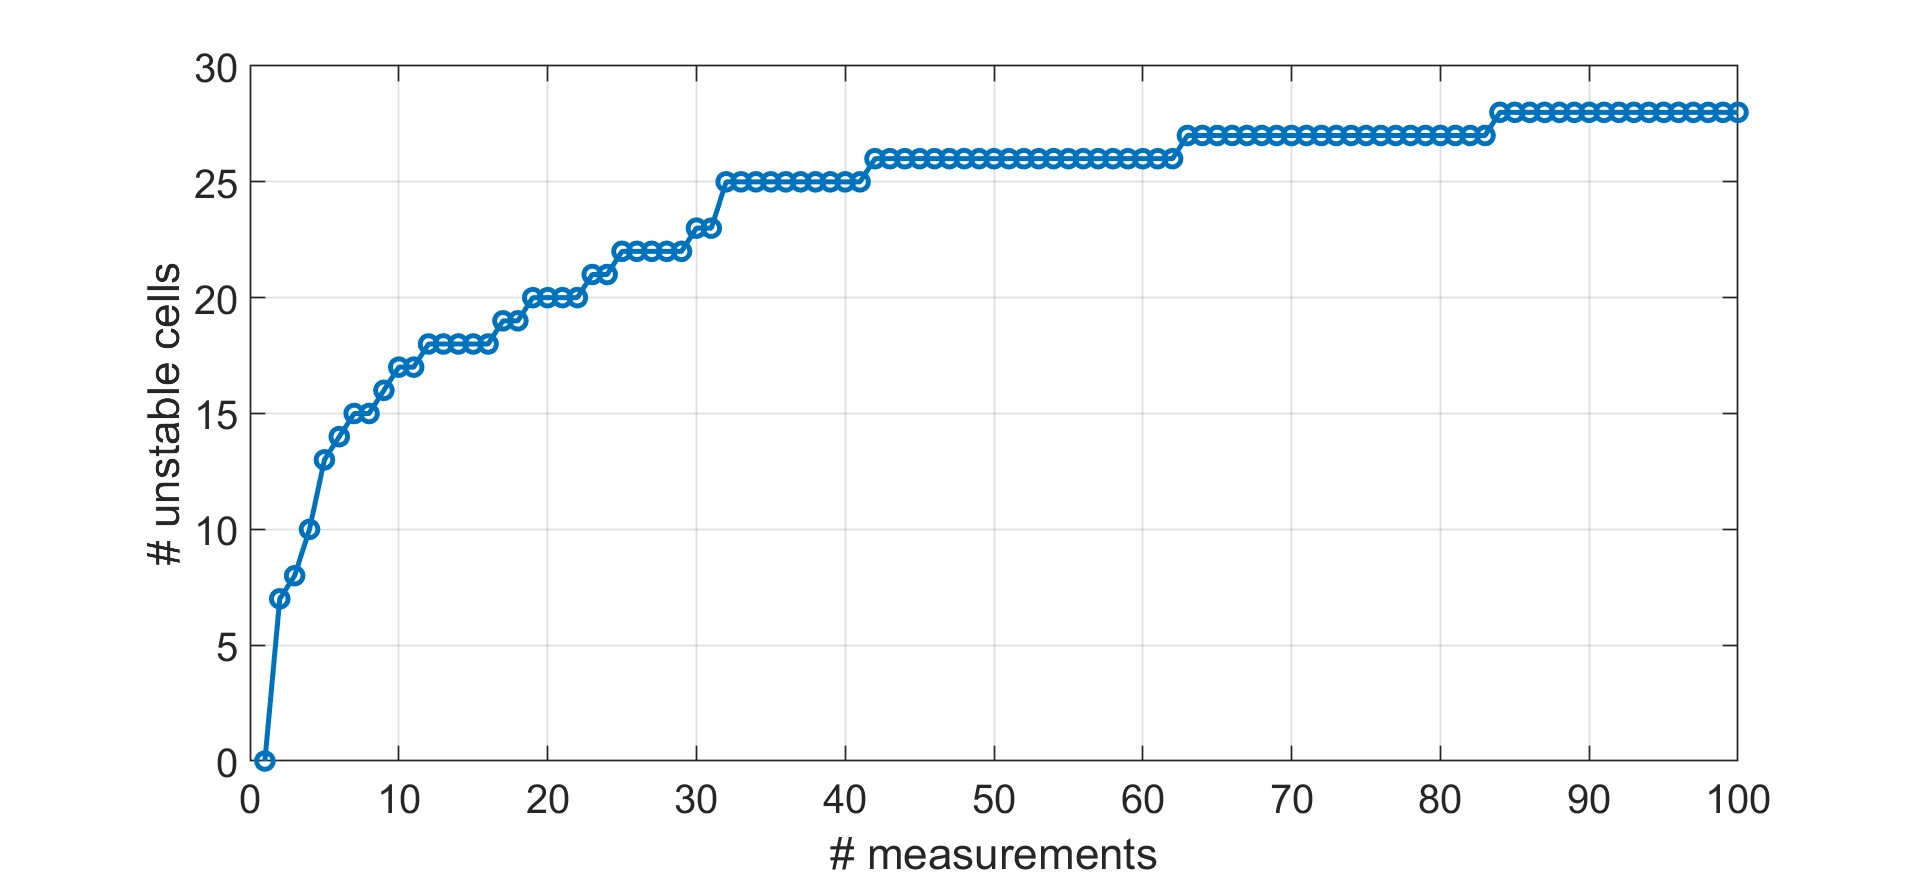
\includegraphics[width=16.5cm]{images/unstalbe_me.jpg}
    \caption{Number of unstable SRAM cells with respect to the number of power-ups for one of the chips. }
    \label{fig:unstable_me}
\end{figure}

\section{Data remanence}

The technique presented in \cite{Liu2017} consists of two remanence tests: writing ‘1’ (or ‘0’) to the entire SRAM cell array and shutting down the power supply for a short time interval until a few cells flip. The technique exploits the fact that the cells that flip with shorter power-off durations have the strongest tendency towards the value that has not been written. This methodology has proven to be effective for experiments performed under different temperatures and power ramp times, and under device aging \cite{Liu2017}. This approach has been tested in a design fabricated in an ultra-low leakage technology, which requires relatively long power-down times (in the order of hundreds of milliseconds) to observe those bit flips. However, much shorter data remanence times are expected for SRAMs built in advanced CMOS technologies (e.g., below microseconds \cite{Liu2017}), which may turn this technique impractical to use on certain technologies. If power-on and power-off times in the order of microseconds have to be precisely controlled, it is clear that the ramp rates must be much faster than that. However, in \cite{Wang2018}, it is shown that the power-up states are especially sensitive to such factors like noise when ramp rates in the range of nanoseconds to microseconds are used. An option to overcome this issue is to operate these tests at low temperatures, at which longer remanence times are expected \cite{Anagnostopoulos2018}. To this end, temperatures of tens of degrees Celsius below zero are necessary, which usually involve the utilization of liquid nitrogen as cooling method. This makes the method further unfeasible for practical applications. Moreover, to control the power-on and power-off times precisely, an additional microcontroller must be used. Therefore, this solution is not suitable for applications with resource-constrained devices.


\section{Exploting the Power Supply Ramp Rate}
\label{sec:bitselection:supply_ramp}
In \cite{Wang2018}, a method to calibrate the strength of the SRAM cells is presented. Its authors claim that, if the SRAM is turned on by ramping the $V_{DD}$ node from low to high at a rapid rate, the power-up of individual cells is decided entirely by the threshold voltage mismatch in the PMOS transistors in each cell. On the other hand, if the SRAM is powered up by rapidly ramping the $V_{SS}$ node from high to low, the power-up state of each cell will depend on the threshold voltage mismatch between the NMOS transistors in the cell. Otherwise, if a slow ramp is used (‘over several seconds’ in \cite{Wang2018}), both NMOS and PMOS pairs play a role in determining the state stored on the cell after the power-up.


From that theoretical starting point, the following method is proposed to identify the strongest cells: first, a fast $V_{DD}$ ramp test is performed to investigate the preferred power-up state of each cell as determined only by its pair of PMOS core transistors. Then, an equivalent test is performed, this time ramping down the $V_{SS}$ -node from high to low, to identify the preferred power-up state as determined only by its pair of NMOS core transistors. Considering both the preferences of the PMOS and NMOS transistors separately, there are four possible combinations (‘0,0’, ‘0,1’, ‘1,0’, ‘1,1’). Thus, around 50\% of the cells are expected to power-up to the same state in both tests. By selecting these, a set of cells where both the NMOS and the PMOS transistor pairs individually bias the cell to the same power-up state is obtained. Finally, the strength of that set of cells is quantitatively calibrated. For that, the SRAM is written with a logic ‘1’ (or ‘0’) and then $V_{DD}$ is slowly ramped down to a small voltage (e.g., 0.1V).

Then $V_{DD}$ is ramped back again to its nominal value. This process is repeated while varying the lower limit of the supply voltage (e.g., 0.1V, 0.11V, 0.12V, etc.). If the initially written value was ‘1’, cells that have ‘0’ as their preferred value may flip to ‘0’ during the above described process. While cells with a stronger tendency towards ‘0’ may already flip their value at higher values of the decreased $V_{DD}$ (e.g., 0.2V), cells with a weaker tendency will need a lower $V_{DD}$ to flip their value (e.g., 0.1V).

However, there are some limitations to this technique. First, unlike other conventional methods to calibrate the strength of SRAM cells \cite{Bhargava2012,Baturone2015,Liu2017}, it requires the realization of ramps in two different nodes of the SRAM cell $(V_{DD} \ \mathrm{and} \ V_{SS} )$. Second, it requires the utilization of two types of ramps, slow and fast, with ramping rates orders of magnitude apart. This translates into additional hardware resources if the method is to be implemented on-chip. Moreover, the utilization of fast ramps at both supply nodes is counterproductive. While fast ramps are performed in 1 nanosecond in the work presented in \cite{Wang2018}, it is also stated in that work that power-ups performed at such fast ramps are very sensitive to factors such as noise or device degradation. Therefore, the classification performed to select the potential candidates using ramps in the nanosecond scale may be incorrect. Finally, no silicon experimental results that validate the method under real operating conditions are presented in \cite{Wang2018}: only simulation results using a Predictive Technology Model (PTM) for a 32-nm bulk technology, with estimated variability parameters, are provided. Moreover, background noise, supply voltage variations, circuit noise, temperature variations or circuit degradation due to aging effects were not considered, even though these are known to be critical factors in the performance of SRAM-based PUFs. 


% Other works that follow a similar approach and their results. 1-2 Pages

% To investigate the effect that a limited number of evaluations has on the determination of the cell strength, a simple Multiple Evaluation test has been performed with the experimental setup used in this work (see Section IV). Figure 2 shows the number of unstable cells with respect to the number of performed evaluations for one of the chips. A similar behavior has been found for all measured chips.

% Considering five different samples of the same chip containing 832 SRAM cells each, the average number of unstable cells after 10 evaluations is 15, while this number increases to 26 after 100 evaluations. Therefore, a reduced number of evaluations will detect only a portion of the unstable cells.

% From the outcome of this test, it becomes clear that a number of evaluations in the order of the ones proposed in [6] or [7] would lead to label some cells as “strong” when in fact these present a relatively high probability of powering-up to their non-preferred value.

% There is another limitation of this method that should be addressed. As it will be shown in Section V, fresh cells (i.e., not aged) that always return the same value when poweredup, may lose their stability after circuit aging, or in the presence of temperature and/or supply voltage variations.

% This fact makes the Multiple Evaluation method unable to find SRAM cells that are truly resilient to these phenomena and, therefore, not suitable for creating a PUF instance.

\section{Maximum Trip Supply Voltage (MTSV) method}
\label{sec:MTSV}
A new bit selection technique is now described. First, a description on how it works is provided. This technique is then tested experimentally against the most popular one available, multiple evaluation. The experimental setup used for these tests is described, and then the results are presented. 


%Detailed description of MTSV. 2-3 Pages.
\subsection{Description}

To overcome some of the limitations that the above-discussed methods present, a new approach is described in this section. The idea behind this method, which will be referred here as MTSV method, is to evaluate the strength of a cell by writing its non-preferred value on it, then lowering $V_{DD}$ for a given period of time, raising it again and checking if the cell has changed its value.

 For the sake of illustration, two cells, \textit{cell1} and \textit{cell2}, which tend to go to ‘0’ but with different strength, will be considered. A ‘1’ is written in both cells and then $V_{DD}$ is lowered and then raised (to its nominal value) repeatedly (with $V_{DD}$ dropping to a lower value with each repetition) until the cell flips its power-up value to ‘0’. It is found that \textit{cell1} flips at $V_{DD1}$ while \textit{cell2} does it at $V_{DD2}$. \textit{Cell1} is said to have a stronger tendency to the ‘0’ state if $V_{DD1}>V_{DD2}$. Therefore, the idea is to classify all the cells in an SRAM by writing their least-preferred value on them, lowering their supply voltage to different values, and recording at which voltage value each cell starts flipping to its preferred value. This voltage value is their data retention voltage (DRV); strongest cells will thus be those with a higher DRV. Cells that, while lowering their $V_{DD}$ at different values during the MTSV procedure, show a random behavior, for example returning ‘0’ and ‘1’ alternatively at different values of decreased power supply, do not have a strong power-up tendency. Therefore, they are labelled as unstable, no DRV value is assigned to them and do not even enter the power-up strength classification procedure.

While the Multiple Evaluation methodology introduced in the previous section may require a prohibitively high number of evaluations, the technique used in this work, on the other hand, requires a much lower number of iterations. For instance, if the range of supply voltages within which the cells experience a bit flip is bounded between ~\SI{80}{mV} and ~\SI{280}{mV} (as it is the case of this work), and assuming a step size of \SI{10}{mV} for the evaluation, a total number of 21 steps is needed. Additionally, unlike \cite{Liu2017}, no precise timing of the power-off and power-on durations is needed, which becomes especially critical when these are in the range of nanoseconds to microseconds. Finally, unlike the method in \cite{Wang2018}, only one type of ramp in one of the nodes is needed. This is important in different aspects. First, only ramps at the SRAM $V_{DD}$ node are performed (no ramp at the $V_{SS}$ node is required). Second, only one ramp rate is needed, while in \cite{Wang2018} two different ramp rates that are orders of magnitude apart were needed.

Furthermore, the ramp used in this work is in the order of a few milliseconds, which results in a reproducible PUF response, while the method in \cite{Wang2018} used fast ramps in the range of nanoseconds, thus producing PUF responses that are very sensitive to factors such as noise or device aging. Finally, by not selecting the candidate cells only among those where both PMOS and NMOS transistor pairs produce a bias towards the same power-up state, potentially stable cells are not discarded, as it occurs in \cite{Wang2018}.



\subsection{Chip}
\label{sec:chip}
The circuit used in this work is an array of 832 SRAM cells, a photograph of which is depicted in Figure \ref{fig:KIPTsram} \cite{Saraza-Canflanca2018}. These cells are distributed in 32 rows by 26 columns. The 6T SRAM cells have been sized with W = \SI{80}{nm} and L = \SI{60}{nm} for the access transistors and the PMOS pull-up transistors, and W = \SI{160}{nm} and L = \SI{60}{nm} for the NMOS pull-down transistors, following conventional sizing criteria. The chip has been designed so that individual access and control of every terminal of each SRAM cell is granted, as shown in fig. \ref{fig:KIPTsramcell}. This is necessary to properly perform the different tests on each SRAM cell, including normal operation tests, aging tests or simply switching off the cells. 

\begin{figure}[H]
    \centering
    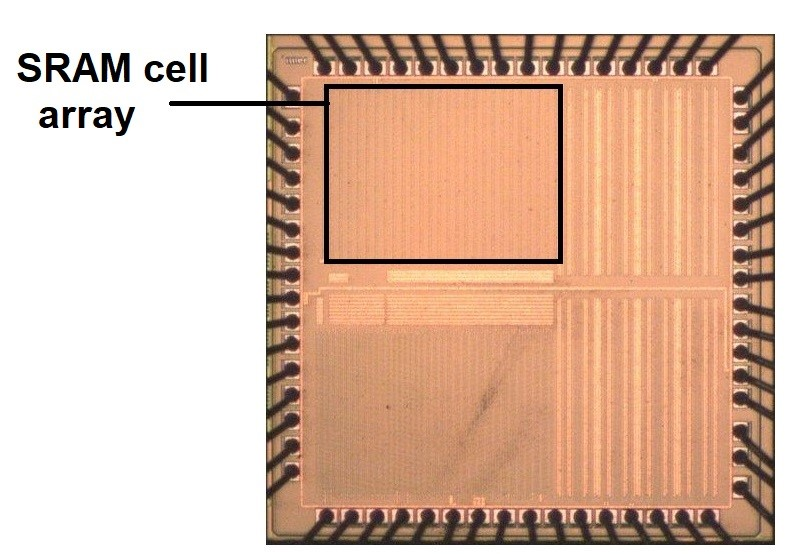
\includegraphics[width=10cm]{images/KIPTsram.jpg}
    \caption{Photograph of the chip used in this work, with the part corresponding to the array of SRAM cells highlighted.}
    \label{fig:KIPTsram}
\end{figure}

For the aging tests, as the degradation of the SRAM operation will extend along years, physical characterization is not possible under normal operation conditions. Therefore, accelerated aging conditions, e.g., by using higher operating voltages on SRAM terminals and/or higher operating temperatures, are applied during certain periods of time, in the range of seconds to hours. Some SRAM figure-of-merit must be measured before and after the stress cycle to compute its degradation.

\begin{figure}[H]
    \centering
    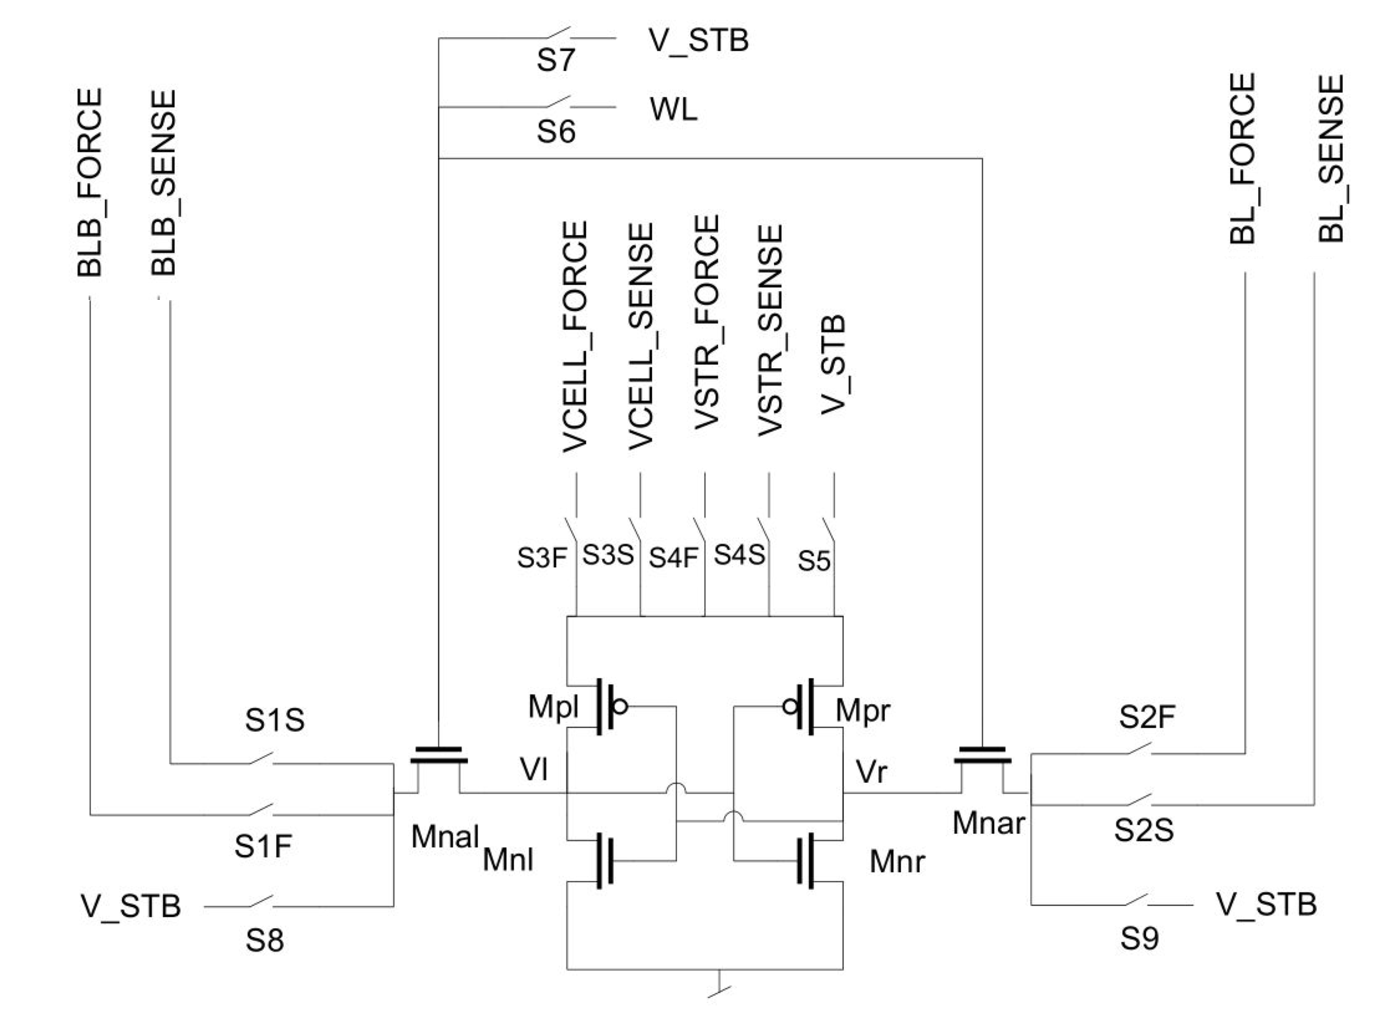
\includegraphics[width=10cm]{images/KIPT cell modified.pdf}
    \caption{SRAM cell with transmission gates for appropriate terminal
access and control.}
    \label{fig:KIPTsramcell}
\end{figure}



It must be noticed that, as explained in section \ref{sec:aging}, in some aging phenomena, e.g., BTI, the stressed devices start recovering their original electrical parameters, once the stressed condition is removed. Therefore, accurate timing of stress and measurement stages must be established. Because of the stochastic nature of aging phenomena, stress and characterization tests must be performed over a large number of devices. The fact that a large number of cells have to be stressed during relatively long times implies a characterization bottleneck if the process is performed serially, cell by cell, especially if the recovery period has to be measured since cells are read-out serially. For this reason, each cell included digital control circuitry that allows parallelization of stress of several cells, while read-out of another cell is performed, strongly reducing the time of these experiments. As an example, if accelerated aging conditions are applied for 10,000 s, it would take around 97 days to characterize all 832 cells serially and around 28 hours to do so parallelly.

Force and Sense (F\&S) techniques are needed for accurate measurements. Therefore, independent F\&S paths are required to access those terminals where current is flowing and a voltage drop can occur.
 
The array includes row and column decoders to individually select each SRAM cell. Digital control circuitry is included in each cell as well as access circuitry (transmission gates, TG) that connect each terminal of each cell to output pads, as shown in Figure 4.3. Four control bits are used to control the TG´s at each node of the SRAM cell, defining 4 different operation modes for each cell: 

\begin{enumerate}
    \item \textbf{Measure mode:} This operation mode has been designed to connect the word line and bit line terminals to the word-line and bit-line analog paths, respectively, and the cell power supply terminal to the standard power supply path. In this operation mode, the selected cell can undergo any write or read operation, or hold some data. Voltages can be fully controlled so that any SRAM figure-of-merit can be properly measured.
    \item \textbf{Stress hold mode:} This operation mode has been designed to connect the power supply terminal of the SRAM to the stress power supply path. As shown in Fig. 3, this path is independent of the standard power supply. This feature enables the parallelization of the stress hold mode of one SRAM cell together with other operations in other cells.
    \item \textbf{Stress AC mode:} This mode has been designed to perform write or read operation under stress conditions, up to 3.3V, applied to the word line, bit lines and power supply terminals.
    \item \textbf{Stand-by mode:} This operation mode connects bit line, word line and power supply terminals to the stand-by analog paths (VSB). This operation mode has been designed to keep all cell terminals at 0V, and therefore under no aging process.
\end{enumerate}



While this modified SRAM cell allows for accurate accelerated aging tests, its characteristics are not different in any way from the standard 6T SRAM cell considered in chapter \ref{chap:3}. The experimental data and conclusions obtained from it can be generalized for a generic SRAM PUF. The MTSV technique itself does not need this particular design. Further information about the circuit design can be found in \cite{Saraza-Canflanca2018}.

\subsection{Experimental setup}
\label{sec:exp_setup}
The main components of the experimental setup used in this work are depicted in Figure \ref{fig:expsetup}. A full-custom Printed Circuit Board (PCB) has been used for the different tests, together with a power supply generator for the biasing of the PCB and the chip. A Keysight B1500 semiconductor parameter analyzer equipped with 4 High Resolution Sense Measurement Units (HRSMU) has been used for voltage application and measurement. The HRSMUs have a F\&S system that, together with the F\&S connection implemented in the circuit, allows the accurate application of voltages by avoiding undesirable voltage drops in the chip. The temperature tests have been performed using an ACS climatic chamber, which allows the stable and homogeneous application of temperature on the chip.

\begin{figure}[t]
    \centering
    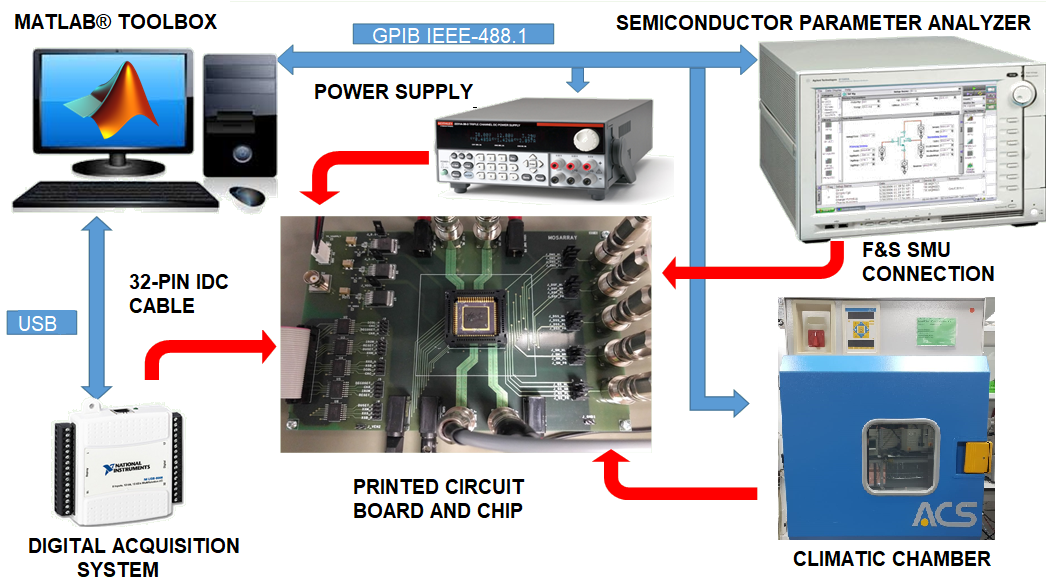
\includegraphics[width=14cm]{images/experimental_setup.png}
    \caption{Representation of the experimental setup used in this work.}
    \label{fig:expsetup}
\end{figure}

\subsection{MTSV experimental performance}

The adequacy of the MTSV method has been tested under four different scenarios: at nominal conditions, after the circuit has been subject to accelerated aging, under temperature variations, and under supply voltage variations. The metrics used to evaluate the quality of the responses are the ones presented in sec. \ref{sec:Metrics}. The values obtained without performing bit selection are the reference point to assess the effectiveness of ME and MTSV. The ramps used in this work are in the order of a few milliseconds, where the power-up state is expected to be scarcely impacted by factors such as noise \cite{Wang2018}. 

\subsubsection{Nominal conditions}

The first step is to measure the response of the chip under nominal conditions of temperature and supply voltage. Five different chips are used during these measurements to ensure that the results are valid under inter-chip variations. Since the inter hamming distance is measured across all chips, it is a good starting point. The result is obtained using eq. \ref{eq:interhd}:

\begin{equation}
\text{mean}_\text{InterHD}=49.9398 \%
\end{equation}

This result is good, close to the ideal 50\%. It confirms that there is no relevant correlation between the power-up behavior of different chips’ cells, and therefore uniqueness is expected from the different PUFs’ responses.

The next step is to classify the cells in terms of their power-up response following the MTSV method. Figure \ref{fig:mtsvflow} shows a flow diagram of how the classification of each cell is done, according to its power-up strength: first, its non-preferred power-up value was written on it. Then, its supply voltage was decreased to different values ranging from $\SI{280}{mV}$ to $\SI{80}{mV}$ and the content of the cell was read at each step. Cells that showed a random behavior, for example returning ‘0’ and ‘1’ alternatively at different values of decreased power supply, were labelled as “unstable”. Among the five chips, the number of unstable cells ranged between 40 and 50 out of the 832 cells of each chip. Interestingly, these cells correspond roughly to the cells labelled as unstable by the Multiple Evaluation method when a large enough number of power-ups is performed (see Figure \ref{fig:unstable_me}). Therefore, cells that did not show a random behavior during the MTSV procedure, that is, cells that flipped their content for one given VDD (their DRV value) and continued flipping their content for any VDD below their DRV value, correspond to the cells labelled as completely stable (0\% erroneous power-ups) by the Multiple Evaluation procedure. These cells were assigned that DRV value and were ordered from strongest (highest DRV value) to weakest (lowest DRV value). Note that the Multiple Evaluation method is not able to perform this classification to the cells it labelled as stable, since they all powered up to the same value at each evaluation. 


\begin{figure}[H]
    \centering
    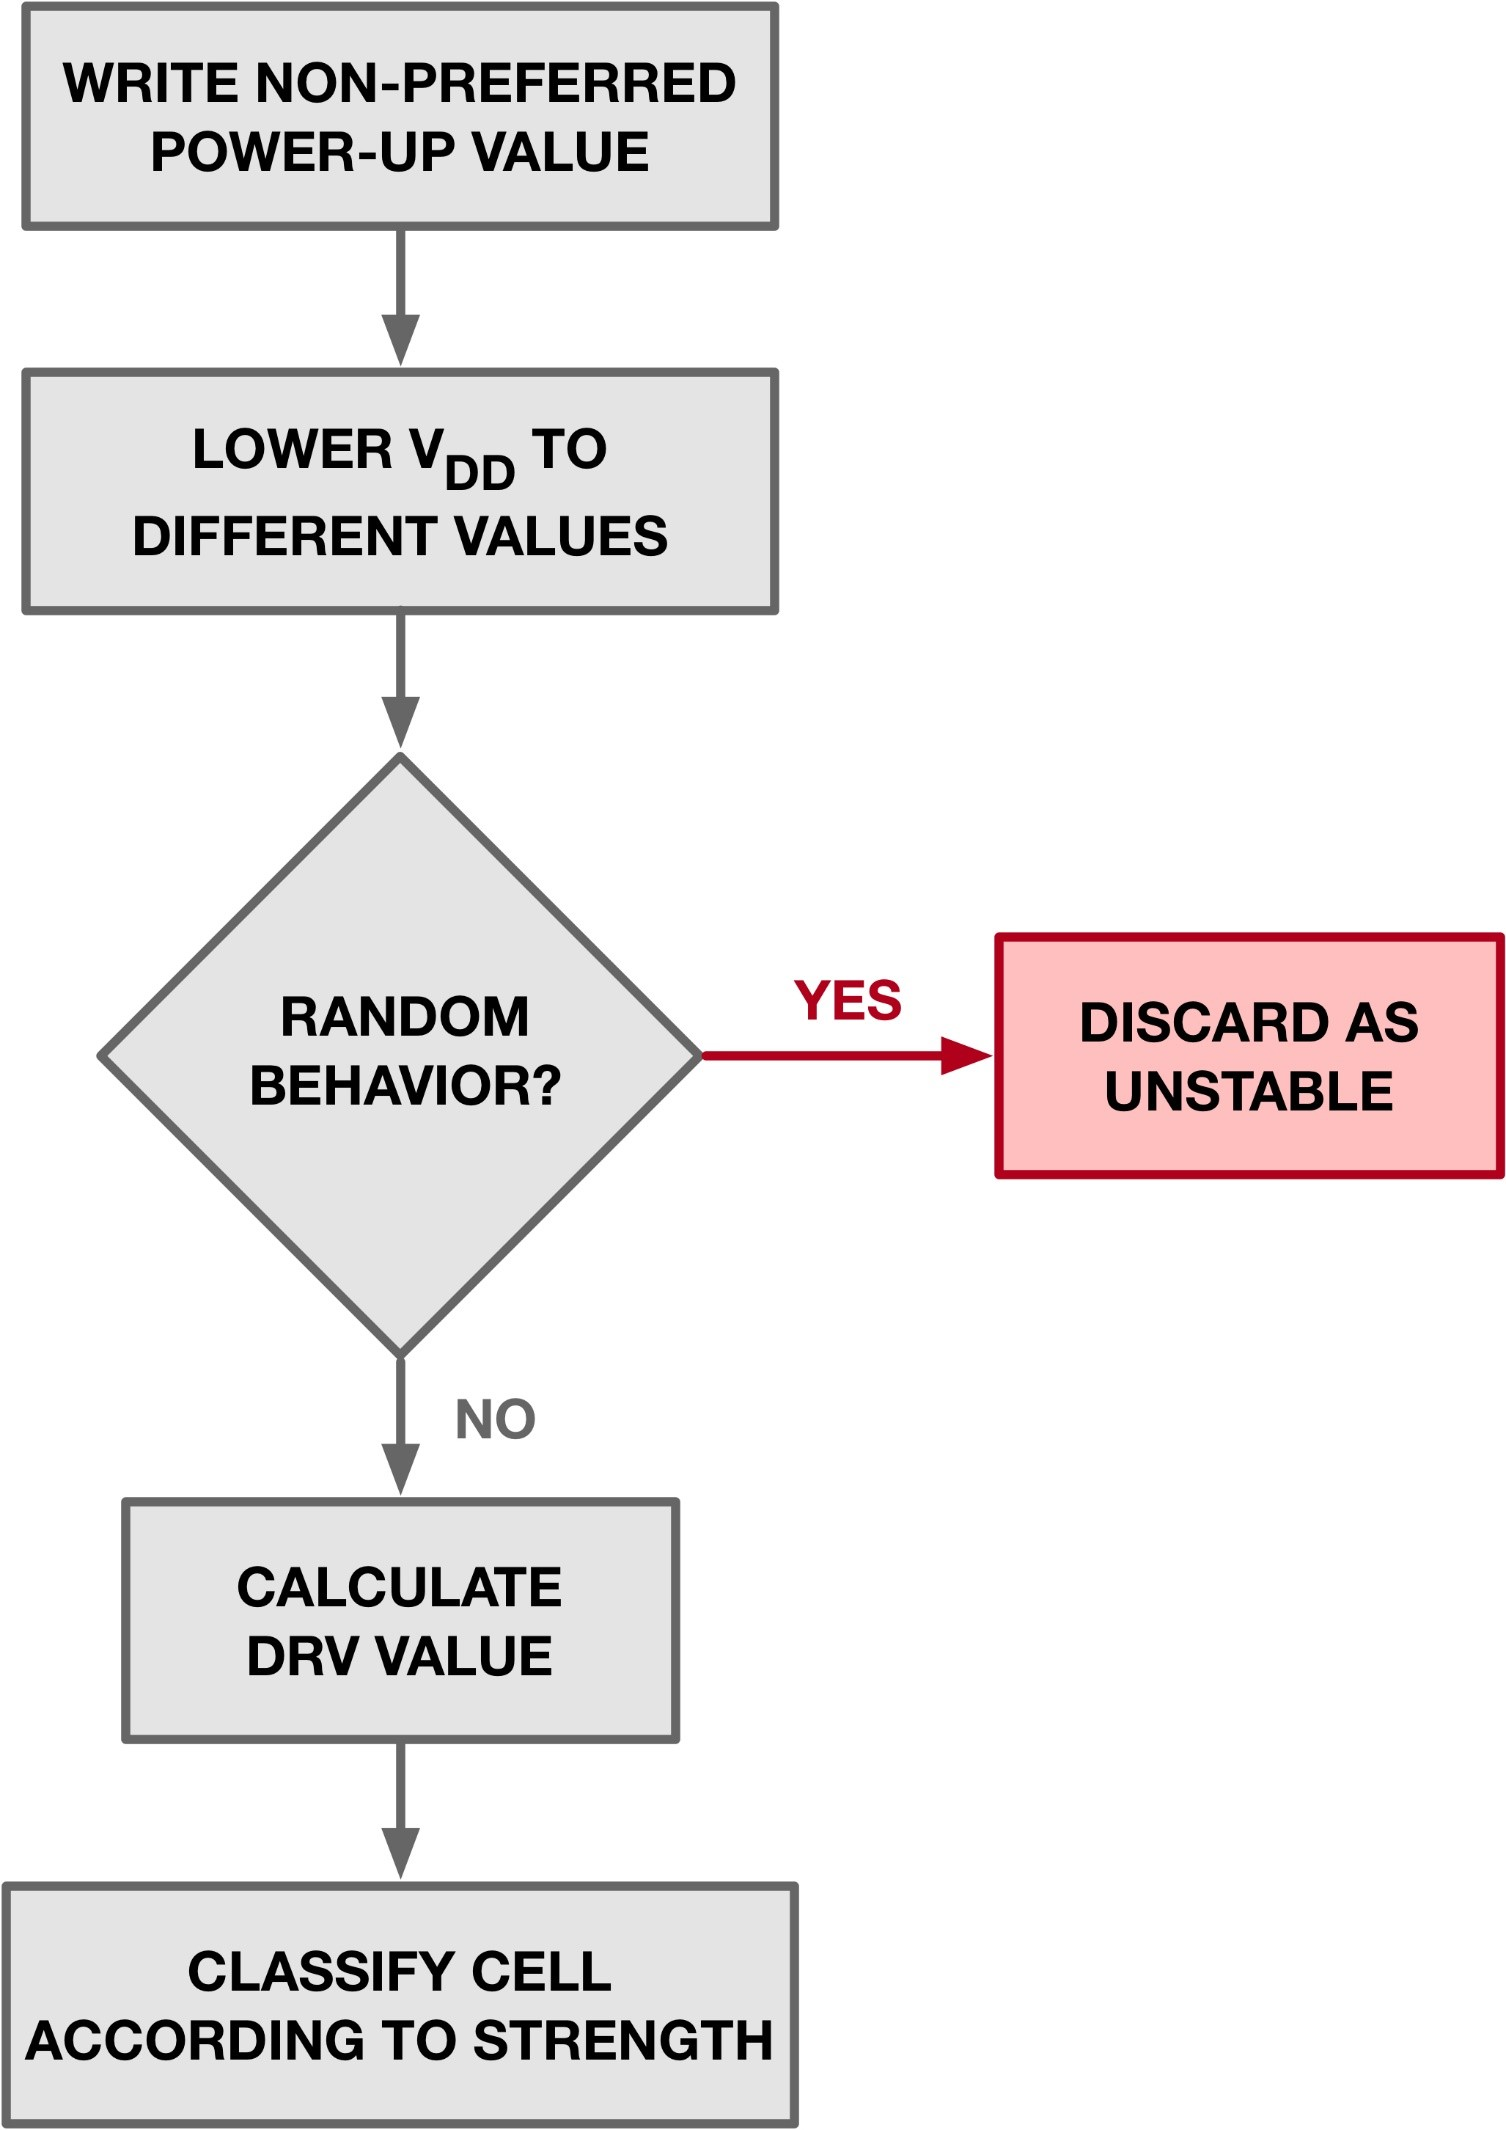
\includegraphics[width=6cm]{images/mtsvflow.jpg}
    \caption{Flow diagram of the procedure used to classify each cell according to its power-up strength. }
    \label{fig:mtsvflow}
\end{figure}

% By the ME approach, cells are labelled as unstable if they do not always return the same value after powering up. The number of unstable cells will increase as more power-ups are performed. Among the five chips the average number of unstable cells after 10 evaluations is 15, while this number increases to 26 after 100 evaluations. Accordingly, a reduced number of evaluations will detect only a portion of the unstable cells, as shown in fig.\ref{fig:unstable_me}. These cells correspond roughly to the cells labelled as unstable by the Multiple Evaluation method when a large enough number of power-ups is performed. Therefore, cells that did not show a random behavior during the MTSV procedure, that is, cells that flipped their content for one given $V_{DD}$ (their DRV value) and continued flipping their content for any $V_{DD}$ below their DRV value, correspond roughly to the cells labelled as completely stable (0\% erroneous power-ups) by the Multiple Evaluation procedure. These cells were assigned that DRV value and were ordered from strongest (highest DRV value) to weakest (lowest DRV value). Note that the Multiple Evaluation method is not able to perform this classification to the cells it labelled as stable, since they all powered up to the same value at each evaluation. Naturally, if no bit selection technique is used the unstable cells are included in the pool of available cells which significantly worsens the quality of the response. 

In order to evaluate the method, the 50 strongest and the 50 weakest cells of each chip were selected, so that their strength could be compared between them and also to the rest of the array. In the following, “weakest cells” refers to the weakest cells among the ones that were not labelled as “unstable” during this first phase of the MTSV procedure. 

It must be noted here that selecting 50 cells has been an arbitrary decision, since a larger or a smaller selection would serve as well for the purpose of this experimental validation. The goal here is not to create a specific PUF instance, but to prove that the MTSV method allows the selection of the strongest and more robust SRAM cells.

Figure \ref{fig:DRVhist} shows a histogram of the DRV values for the SRAM cells that display a tendency to power-up to one of the possible values. The histogram corresponds to an MTSV experiment with $V_{DD}$ step size of \SI{5}{mV}, performed on 832 cells of one of the chips. The strongest cells correspond to the right tail of the histogram, i.e., those with a higher DRV value, while the weakest cells correspond to the left tail of the histogram. Unstable cells do not appear in the histogram, since no DRV value could be assigned to them.

\begin{figure}[t!]
    \centering
    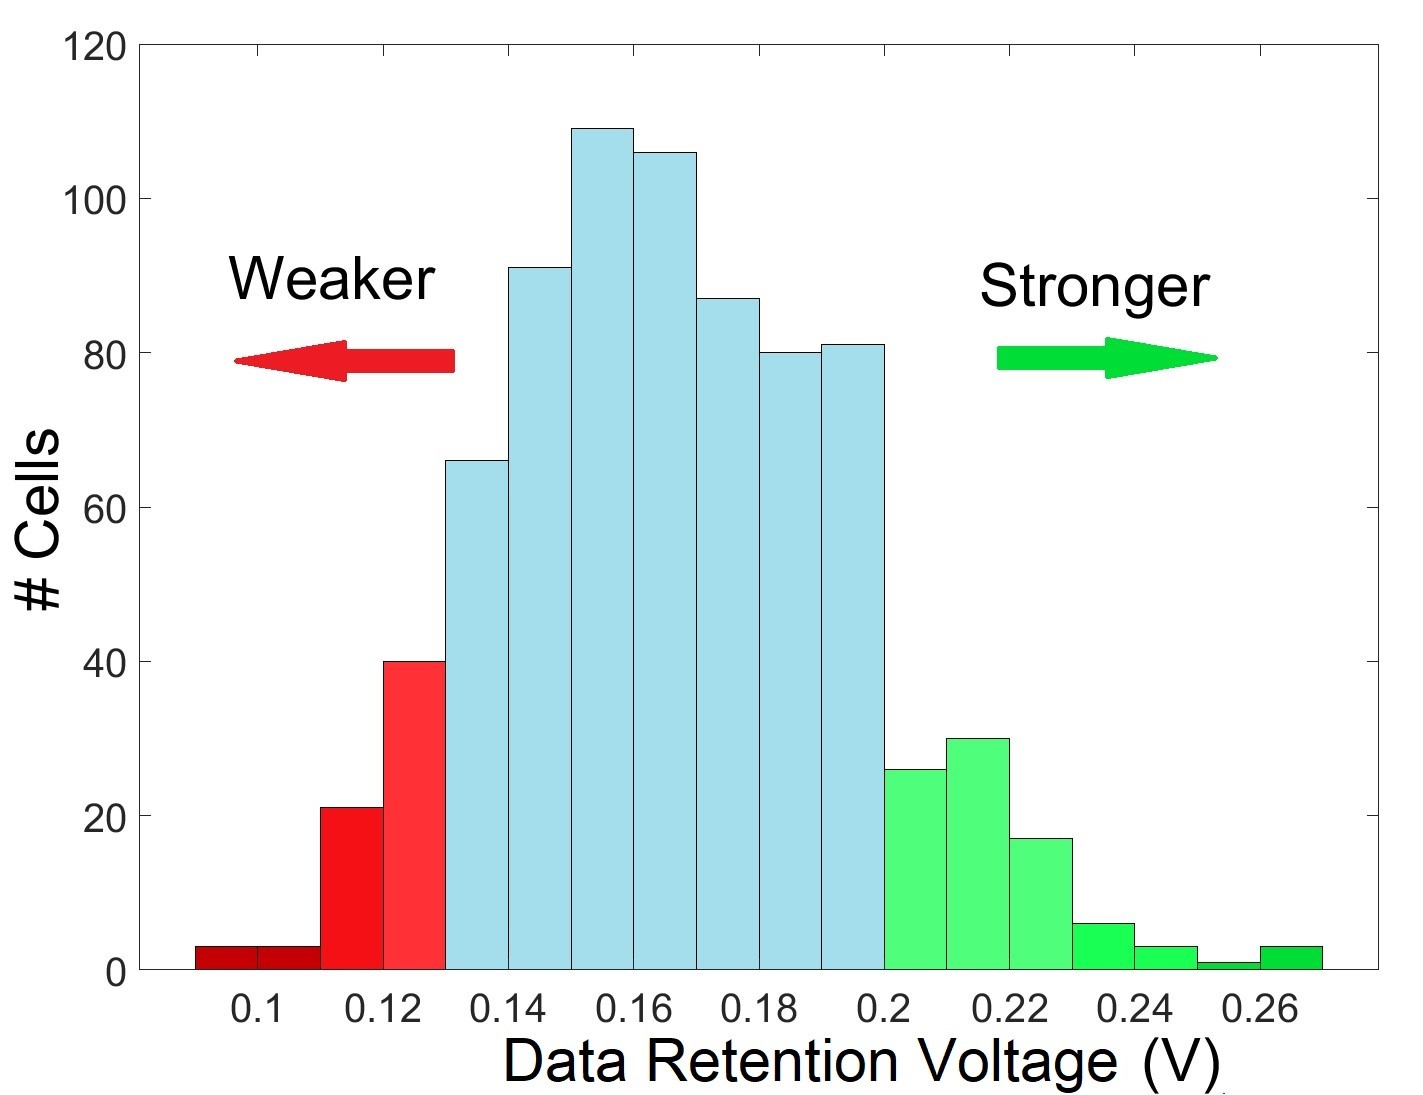
\includegraphics[width=12cm]{images/DRV histogram.jpg}
    \caption{Histogram of the $V_{DD}$ values at which cells (in one of the chips) start flipping from their non-favorite to their favorite value. }
    \label{fig:DRVhist}
\end{figure}


Then, to evaluate the adequacy of the MTSV-based classification, 2,500 power-up evaluations are performed for the 50 strongest and the 50 weakest cells of each chip, and 200 power-ups for the rest of cells. The number of power-ups applied to the strongest and weakest cells is higher than the one commonly used in the Multiple Evaluation method, but for the purpose of the comparison made here, this number will provide a much more precise evaluation of the cell strength. Table \ref{tab:Nom_ave_BER} contains information about the mean BER obtained for the chips considering i) all the cells, ii) only the unstable ones, iii) the 50 strongest ones and iv) the 50 weakest ones. It is important to remember that “weakest” refers to the weakest cells once the unstable cells according to the MTSV method have been discarded. That is why the 50 weakest cells perform better than the complete array. The sets of strongest and weakest cells display proportionally fewer errors than the complete array or the set of unstable cells, so a larger number of evaluations was necessary to achieve the adequate accuracy. These results are displayed in Figure \ref{fig:BERhistSnW} in a more visual manner. Notice that, for a clearer visualization, Figure \ref{fig:BERhistSnW} has been plotted in logarithmic scale due to the large disparity of BER values, which span across several orders of magnitude. This occurs because cells classified as the strongest by the MTSV method have extremely low (i.e., good) BER values. 


\begin{table}[H]
  \centering
  \caption{Mean value of BER for the five chips}
  \vspace{5mm}
    \begin{tabular}{|c|c|c|c|c|}
    \hline
     & All cells & Unstable cells & 50 weakest cells & 50 strongest cells \bigstrut\\
          \hline
    %  \#1 & 0.3430 \% & 8.8556 \% & 0.0036 \% & 0.0064 \% \bigstrut\\
    %     \hline
    %  \#2 & 0.5265 \% & 8.8556\%  & 0.0765 \% & 0.0025 \% \bigstrut\\
    %     \hline
    %  \#3 & 0.3430 \% & 7.0500 \% & 0.0036 \% & 0.0064 \% \bigstrut\\
    %     \hline
    %  \#4 & 0.5265 \%  & 8.8556 \% & 0.0765 \% & 0.0025 \% \bigstrut\\
    %     \hline
    %  \#5 & 0.5265 \%  & 8.8556 \% & 0.0765 \% & 0.0025 \% \bigstrut\\
    % \hline
    BER (\%) & 0.5265  & 8.8556  & 0.0765  & 0.0025  \bigstrut\\
    \hline
    \end{tabular}%
  \label{tab:Nom_ave_BER}%
\end{table}%


\begin{figure}[H]
    \centering
    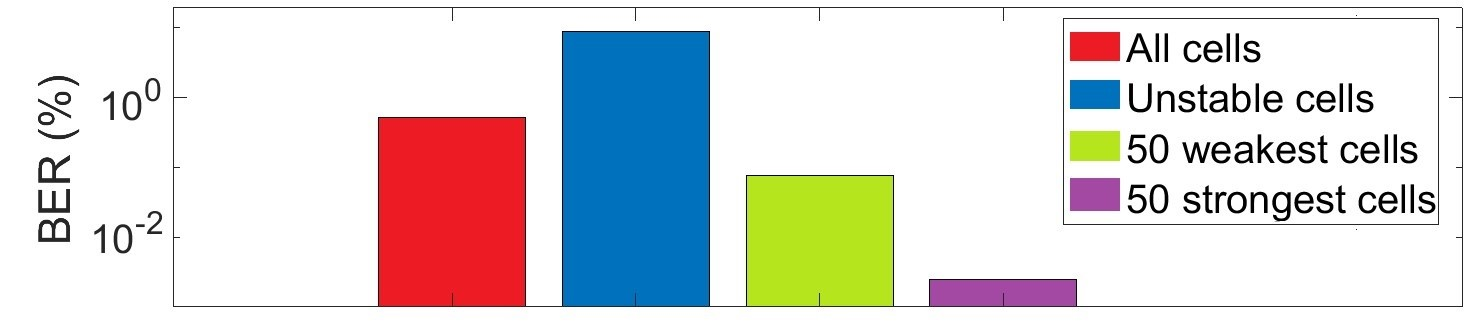
\includegraphics[width=10cm]{images/histBERSnW.jpg}
    \caption{Average BER of the five chips taking into account all cells, only unstable cells, the 50 weakest cells and the 50 strongest cells. }
    \label{fig:BERhistSnW}
\end{figure}
The BER results indicate that the cells labelled as unstable during the first step of the MTSV method are those with a larger instability, and that, by just applying the first part of the MTSV procedure and discarding these cells, the reliability of the PUF is largely increased. Once the unstable cells have been discarded, the remaining cells are classified  according to their DRV value, and the strongest ones are selected. Table \ref{tab:Nom_ave_BER} and Figure \ref{fig:BERhistSnW} show that this further improves the reliability of the PUF, since the 50 strongest cells according to their DRV have $\sim30$ times less power-up errors than the 50 weakest ones, and $\sim210$ times less power-up errors than when no classification is done and the whole array is considered.

As a final remark to highlight the strength of the cells selected by the MTSV method, a 0.0025\% BER means that, in average, the strongest cells yield an erroneous power-up only once out of 40,000 times. It becomes thus evident that a typical Multiple Evaluation test with some tens of power-ups, like those in \cite{Bhargava2012,Baturone2015}, would not be able to achieve such a selection. This is the reason for choosing a very high number of power-up evaluations to test the cells that were not discarded during the first part of the MTSV test.
In the following subsections, the capacity of the MTSV method to select strong cells in the presence of circuit aging and temperature and supply voltage variations will be evaluated. For this, the focus will be set on the strongest and weakest cells, since it has already been shown at nominal conditions that the cells labelled as unstable by the MTSV method are not suitable to be used in PUF identifiers.

\subsubsection{Resilience to circuit aging}
\label{ss:aging}

The next step was to evaluate the adequacy of the MTSV method to select aging-resilient cells. For this, the 100 selected cells (50 strongest and 50 weakest) of one of the chips (chip \#1) were stressed (i.e., aged in an accelerated manner) to reinforce their non-preferred value. It must be clarified that this does not aim at emulating a real-case operation scenario, since SRAMs will age in different manners depending on the application they are used for. Therefore, the goal of this test is to represent a worst-case of aging degradation, in which its impact systematically reduces the cell power-up strength. To achieve this, their preferred value was written on each cell, and then the supply voltage was raised to \SI{2.5}{V} during 10,000 s. As mentioned in chapter \ref{chap:3}, the BTI aging suffered by an SRAM cell that stores a given value (e.g., ‘0’) drives the preferred power-up value of that cell towards the opposite value (e.g., ‘1’) \cite{Bhargava2012}. This aging is $V_{GS}$-activated, and can be accelerated by increasing this voltage over its nominal value (1.2V for the technology used in this work). This is achieved by increasing the supply voltage of the cell. After this high voltage is removed, there are both a permanent and a recoverable component of degradation. For this reason, several measurements have been performed to investigate the resilience of the cells against degradation: one right after the stress ended, and three additional measurements 3 days, 10 days and 40 days later, to observe the evolution of the power-up behavior during the BTI recovery. The experiment performed right after the end of the stress consists of only 150 power-ups so that the recovery of the degradation throughout the test is not very significant. The other experiments, performed some days/weeks after the end of the stress, consist of 2,500 power-ups for each cell. The results obtained for each test were compared to the golden response obtained at nominal conditions for that chip before the stress was applied. The results for these experiments are collected in Table \ref{tab:aging_ave_BER}.

\begin{table}[H]
  \centering
  \caption{Average BER of the 50 strongest and 50 weakest cells of chip \#1 after accelerated aging}
  
  \vspace{5mm}
    \begin{tabular}{|c|c|c|c|c|}
    \hline
     Time after stress & Right after stress & 3 days & 10 days & 40 days \bigstrut\\
    \hline
    BER (\%) 50 strongest & 0 & 0 & 0.0016 & 0.0008 \bigstrut\\
    \hline
    BER (\%) 50 weakest & 28.1200 & 21.0424 & 19.2640 & 18.5720 \bigstrut\\
    \hline
    \end{tabular}%
  \label{tab:aging_ave_BER}%
\end{table}%

In this case, the difference in resilience against accelerated aging between the cells classified as strong and weak by the MTSV method is quite revealing. The 50 strongest cells according to that method remain unaffected by aging in terms of their power-up response, having a BER of 0 (which means that there was no power-up different to the one in the golden response) or very close to 0 in each experiment. On the other hand, the BER of the 50 weakest cells is much larger than the values obtained at nominal conditions before the stress was applied. Before the stress, this value for all chips was ~0.08\% (see Table \ref{tab:Nom_ave_BER}), while now it is ~28\% right after the stress, and it slowly recovers down to ~19\%. This large increase in BER for the cells classified as weakest by the MTSV method, while those classified as strong maintain a very low BER, indicates that the MTSV method has correctly selected the cells that are more resilient to circuit aging in terms of power-up response. Notice that, according to the Multiple Evaluation method, both sets of weakest and strongest cells had been labelled as equally strong, since they both had 0\% erroneous power-ups at nominal conditions. This demonstrates how the MTSV is able to foresee, before the cells have suffered any type of aging, which ones are going to be more robust against it, and therefore proves to be outstanding when selecting cells that are resilient to aging.



To gain insight into how the strength of the cells has changed after the stress, the DRV values measured 10 days after application of the stress are depicted in Figure \ref{fig:DRV_hist_stress}. It can be seen how, although the average DRV of the 50 strongest cells, and with it their strength, decreases slightly after the application of the stress, it is still much larger than the fresh DRV of the 50 weakest cells. This explains the fact that, even after the stress, the cells classified as strongest by the technique proposed in this work still have a strong tendency towards the same value when powered up. On the other hand, the case of the 50 cells classified as weakest is very different. Only 33 out of the 50 weakest cells remain stable after the stress, while the remaining 17 cells lost their tendency towards a given value and, therefore, no DRV could be assigned to them. For this reason, only those 33 weakest cells are shown in the histogram at the bottom of Figure \ref{fig:DRV_hist_stress}. As it can be seen in that histogram, there was also a decrease in their average DRV of a few milivolts.
To shed some light on the behavior of the recoverable component of the degradation, the BER value measured in each of the tests shown in Table \ref{tab:aging_ave_BER} is plotted against the time elapsed from the stress in Figure \ref{fig:BER_ev}. Interestingly enough, the expected logarithmic recovery of degradation at device level (i.e., of the transistors’ threshold voltage) \cite{Rangan2003}, translates into a logarithmic recovery of BER after the application of the stress.


\begin{figure}[H]
    \centering
    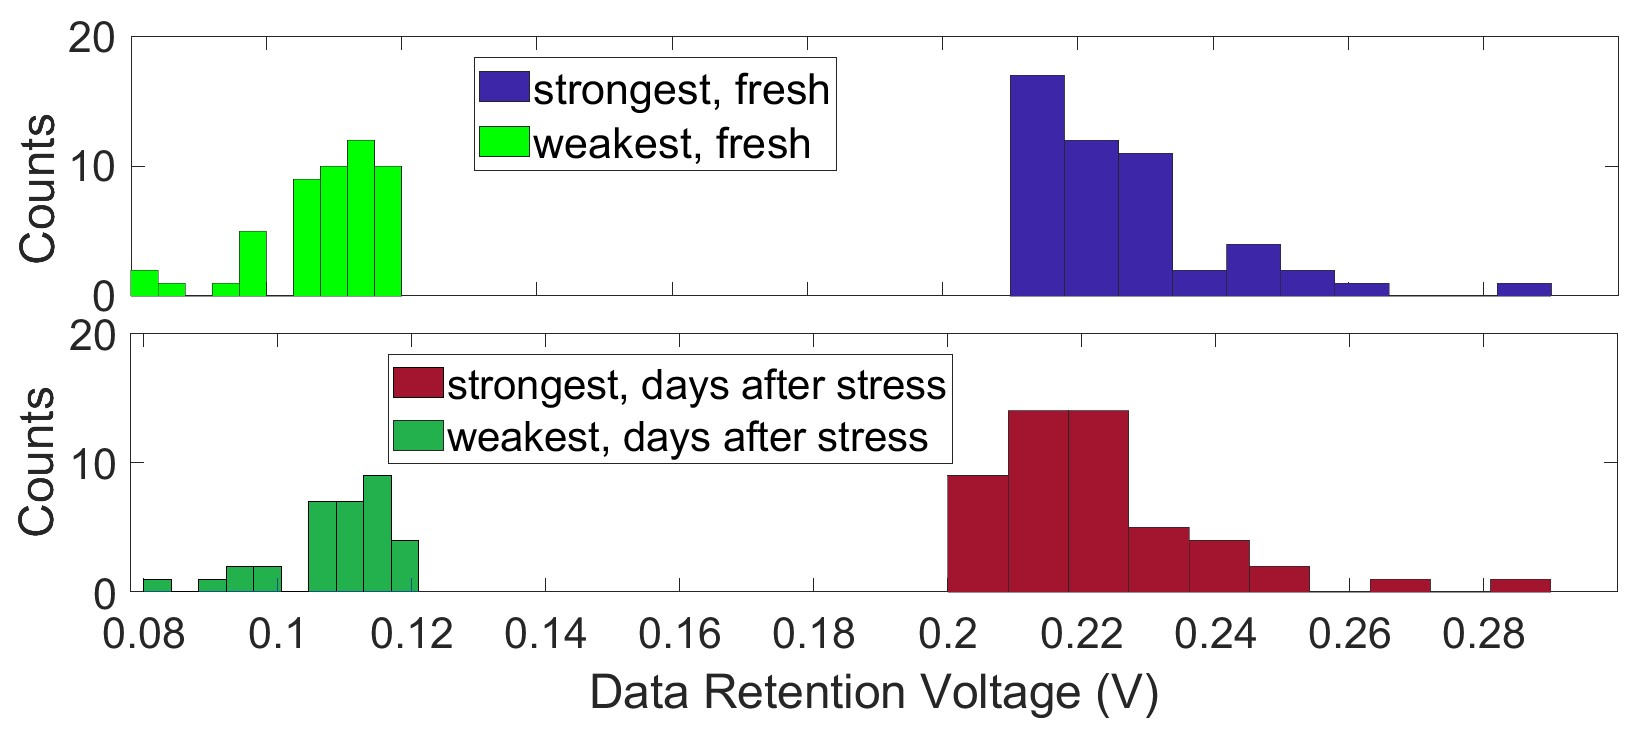
\includegraphics[width=10cm]{images/DRV_hist_stress.jpg}
    \caption{DRV value for the 50 strongest and 50 weakest cells measured before the stress (top), and 10 days after stress removal (bottom). }
    \label{fig:DRV_hist_stress}
\end{figure}

\begin{figure}[H]
    \centering
    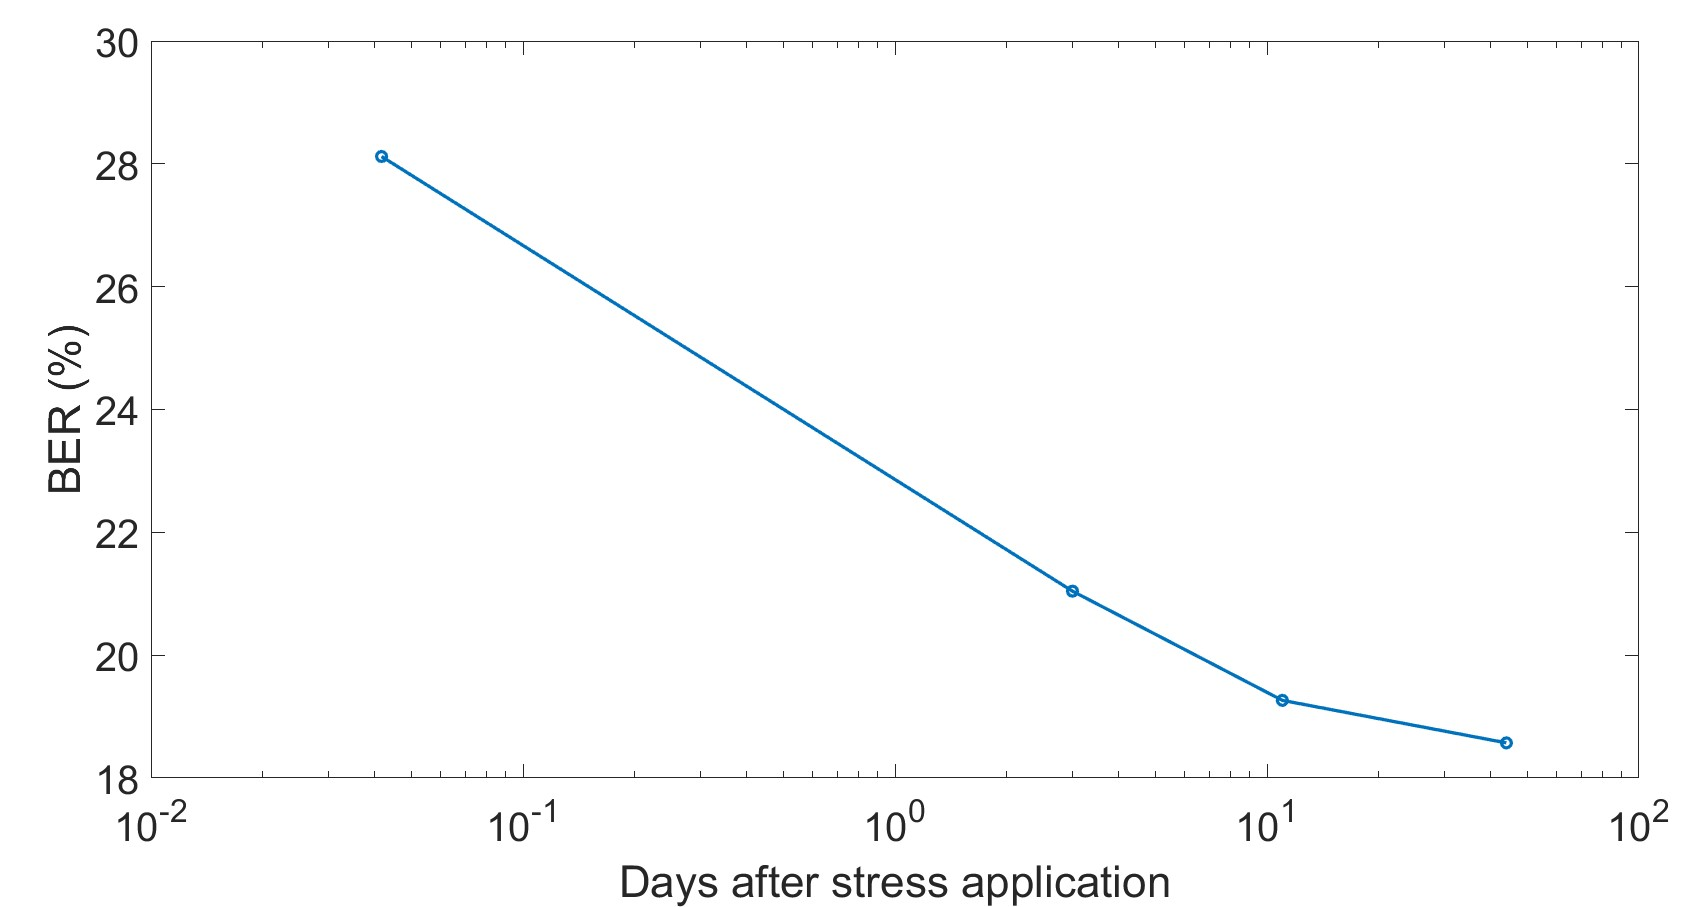
\includegraphics[width=10cm]{images/BER evolution.jpg}
    \caption{BER evolution for the 50 weakest cells of a chip with respect to the number of days since the application of the stress. }
    \label{fig:BER_ev}
\end{figure}

\subsubsection{Resilience to temperature variation}

To test the adequacy of the MTSV method under temperature variations, the 50 strongest and the 50 weakest cells of another chip (chip \#2) were selected under nominal conditions. Then, 2,500 power-ups were performed for each cell at $\SI{0}{\degree C}$, $\SI{10}{\degree C}$, $\SI{20}{\degree C}$, $\SI{30}{\degree C}$ and $\SI{40}{\degree C}$. The power-up response of the cells obtained under the different temperatures was evaluated using as a reference the golden response of that same chip obtained at room temperature, i.e., $\SI{25}{\degree C}$. The BER results are included in Table \ref{tab:temp_ave_BER}. 


Again, the 50 strongest cells according to the MTSV method prove to be very resilient against environmental variations, in this case against temperature variations ranging from $\SI{0}{\degree C}$ to $\SI{40}{\degree C}$. In fact, the worst BER obtained for the 50 strongest cells is 0.0024\%, which is even slightly lower than the average BER for the 50 strongest cells obtained at nominal conditions of temperature and supply voltage, which was 0.0025\%. The 0.0024\% BER obtained in the worst case for temperature variations translates into roughly 1 erroneous power-up out of every 42,000 evaluations. On the other hand, the performance of the cells classified as weakest by the MTSV method worsens when temperature variations are considered. For instance, the BER increases more than 10 times at both $\SI{0}{\degree C}$ and $\SI{40}{\degree C}$ compared to the one found at $\SI{20}{\degree C}$. The worst BER result for the 50 weakest cells is 1.7592\% at $\SI{0}{\degree C}$. This BER value corresponds to roughly 1 erroneous power-up out of every 57. This error rate is ~700 times larger than that of the strongest cells.
Similar to the circuit aging scenario discussed in the previous subsection, the results presented in Table \ref{tab:temp_ave_BER} prove that the MTSV method performed at nominal conditions has been able to correctly select the SRAM cells with a power-up behavior that better tolerate temperature variations. 


\begin{table}[H]
  \centering
  \caption{Average BER of the 50 strongest and 50 weakest cells of chip \#2 tested under temperature variations}
  \vspace{5mm}
    \begin{tabular}{|c|c|c|c|c|c|}
    \hline
     Temperature & $\SI{0}{\degree C}$ & $\SI{10}{\degree C}$ & $\SI{20}{\degree C}$ & $\SI{30}{\degree C}$ & $\SI{40}{\degree C}$ \bigstrut\\
    \hline
    BER (\%) 50 strongest & 0 & 0.0024 & 0.0008 & 0.0024 & 0.0008\bigstrut\\
    \hline
    BER (\%) 50 weakest & 1.7592 & 0.4080 & 0.1256 & 0.2288 & 1.2128 \bigstrut\\
    \hline
    \end{tabular}%
  \label{tab:temp_ave_BER}%
\end{table}%

\subsubsection{Resilience to Supply Voltage Variations}

The final test that has been performed was to test the adequacy of the MTSV method to select cells with a power-up response that is reproducible when supply voltage variations are introduced, since this type of fluctuations may be present in real application scenarios. For this, the 50 strongest and 50 weakest cells of one of the chips (chip \#2) according to the MTSV classification were powered-up 2,500 times each at room temperature and different supply voltages, i.e., raising their supply voltage from ground (\SI{0}{V}) to \SI{1.08}{V}, \SI{1.14}{V}, \SI{1.2}{V}, \SI{1.26}{V} and \SI{1.32}{V}. This corresponds to a range of the nominal voltage $1.2 \ \mathrm{V} \pm 10\%$. As in the previous tests, the results were compared to the golden response of the chip measured at nominal temperature and supply voltage conditions. The BER values obtained for this test are displayed in Table \ref{tab:vdd_ave_BER}. The worst BER value for the 50 strongest cells is obtained at $V_{DD} = \SI{1.2}{V}$ and is 0.0048\%, which corresponds roughly to one erroneous power-up out of every 21,000 power-ups. For the 50 weakest cells, the worst BER value is obtained at $V_{DD}$ = $\SI{1.32}{V}$ and is 0.204\%, 
equivalent to one erroneous power-up out of every 490, which corresponds to an increase in the error rate of ~70\% compared to the one obtained at nominal supply voltage conditions. As in the previous tests, these results make clear that the MTSV classification performed at nominal temperature and supply voltage conditions is able to select cells that will have an extremely reproducible power-up behavior even under supply voltage variations


\begin{table}[H]
  \centering
  \caption{Average BER of the 50 strongest and 50 weakest cells of chip \#2 tested under supply voltage variations}
  \vspace{5mm}
    \begin{tabular}{|c|c|c|c|c|c|}
    \hline
     Supply voltage & $\SI{1.08}{V}$ & $\SI{1.14}{V}$ & $\SI{1.20}{V}$ & $\SI{1.26}{V}$ & $\SI{1.32}{V}$ \bigstrut\\
    \hline
    BER (\%) 50 strongest & 0.0024 & 0.0016 & 0.0048 & 0.0008 & 0.0008\bigstrut\\
    \hline
    BER (\%) 50 weakest & 0.1160 & 0.1208 & 0.1216 & 0.1312 & 0.2040 \bigstrut\\
    \hline
    \end{tabular}%
  \label{tab:vdd_ave_BER}%
\end{table}%



\chapter{PUF experimental implementation}
\label{chap:5}
After explaining the fundamental features of silicon PUFs, describing SRAM PUFs and presenting a new bit selection technique, this chapter is focused on presenting a real and complete PUF response. The objective is to verify the assertions made so far by turning the PUF with an unreliable response into a reliable key generator, using MTSV bit selection to alleviate the requirements of the ECC circuitry.

The chip design and the experimental setup used in this chapter are the ones described in subsections \ref{sec:chip} and \ref{sec:exp_setup}. In this case, only one chip (chip \#6) is characterized. Instead of evaluating the 50 strongest and weakest cells according to MTSV, all the 832 cells of the chip will be measured. 

First, different bit selections are considered to be used as a comparison with MTSV-based bit selection. Then, these selections are tested under nominal conditions, as well as under supply voltage variations, temperature variations and accelerated aging. An appropriate ECC will be selected based on the data for each one, and the fuzzy extractor construction will be implemented under different scenarios. Finally, a discussion on the exact ECC requirements for a KER of $10^{-4} \ \%$ based on the measured BER values is presented.

% Along the way other characteristics such as uniqueness and uniformity will be evaluated to ensure that this PUF's response works well as a key and that the conclusions reached in this work can be extrapolated for other designs. 


%Although the 50 strongest cells and 50 weakest cells were useful to prove the merits of MTSV as a bit selection technique, the 50 weakest cells are precisely the ones to avoid in the response and having only 50 bits of response from the 50 strongest is insufficient as explained in subsection \ref{sec:enc/dec}. 


\section{Bit selections}

The first step is to decide the key-length. It is important to remember that our chip has 832 cells to select from, while commercial SRAMs will generally have many more \cite{Schrijen2012}. A length of 128 bits is the bare minimum for cryptographic algorithms, as explained in sec. \ref{sec:enc/dec}, and it will be the benchmark used. 

%It is important to remember that our chip has 832 bits to select from, while commercial SRAMs will generally have many more \cite{Schrijen2012}. Since MTSV provides a classification of the reliability of the cells, more cells available means better results. 

Next, the required BER out of each selection must be calculated. It is tied to the target for KER, which was set at lower than $10^{-4} \ \%$ in sec. \ref{sec:HDAs}. The KER is understood as the probability of obtaining an erroneous key, which translates to the probability of an error in one or more bits. This probability can be derived by evaluating the binomial distribution (eq.\ref{eq:binomialpmf}) term by term and performing approximations. 

% This equation is shown again to facilitate the explanation:

% \begin{equation*}
% P(x=k)=
% \left(\begin{array}{l}
% n \\
% k
% \end{array}\right) p^{k}(1-p)^{n-k}\end{equation*}

Naturally, $P(x=k)=10^{-4} \ \%$. Using the approximation found in eq. \ref{eq:prob}, the probability of failure of each bit $p$ can be approximated to the average BER of the response $(p\approx \mathrm{BER})$ \cite{Maes2009}. This is a naive approach, since error rate will not be homogeneous across all cells \cite{Delvaux2015}. For example, if one cell had 100\% BER but the rest had 0\%, the average BER of a 128-bit string would be 0.78\% according to eq. \ref{eq:BER}. The failure rate would be 100\% since one cell always fails, but it would not appear so by using the overall BER. However, it is an extreme case and in most cases this approach gives a good first estimation on the real KER. 

The probability $p$ must be low to meet the strict KER requirement, so presumably $p<<1$ and $(1-p)\approx 1$. $k$, equivalent the number of failures, can be taken as 1 as the probability of two mistakes is negligible for $p<<1$. In this case, the binomial coefficient is simply $ \binom{n}{1} = n $. This results in a target  of $\mathrm{BER}\approx p=n^{-1} 10^{-4} \ \%$ i.e. $\SI{7.8}{\cdot 10^{-7}\ \%}$ for a 128-bit key.

Once the length of the selection and the desired BER are established in an ideal and theoretical way, the next subsections explain the different selections used during the experimental tests.

\subsection{Arbitrary selection}

An arbitrary selection corresponds to a selection that does not follow any reliability criteria. It is meant to serve as a point of reference to compare the other bit selection techniques, and how much the required ECC is reduced by them. They should generally have a reliability close to the global reliability of all cells. Two arbitrary selections are considered: \textit{First} and \textit{Random}. \textit{First} simply takes the first 128 cells of the SRAM array, which would be the fastest to read. \textit{Random} takes a random selection of 128 cells out of the 832 ones available. 

\subsection{Multiple Evaluation selection}

Multiple evaluation is the most popular bit selection technique in the bibliography \cite{Delvaux2015,Baturone2015,Bhargava2012}, so it provides an appropriate comparison for MTSV bit selection. 20 power-ups were used for this selection as suggested by \cite{Baturone2015}. With these power-ups, 21 cells are classified as unstable, leaving 811 to choose from. Fig. \ref{fig:MEunstable_progression} shows how the number of unstable cells increases with each power up.


This technique does not provide a classification of the available 811 ``stable'' cells. A random selection of 128 cells among these 811 ones is taken, \textit{ME Stable}. Fig. \ref{fig:MEselection} shows which cells in the array are considered unstable in red and which ones are chosen for \textit{ME Stable} in green.

\begin{figure}[H]
    \centering
    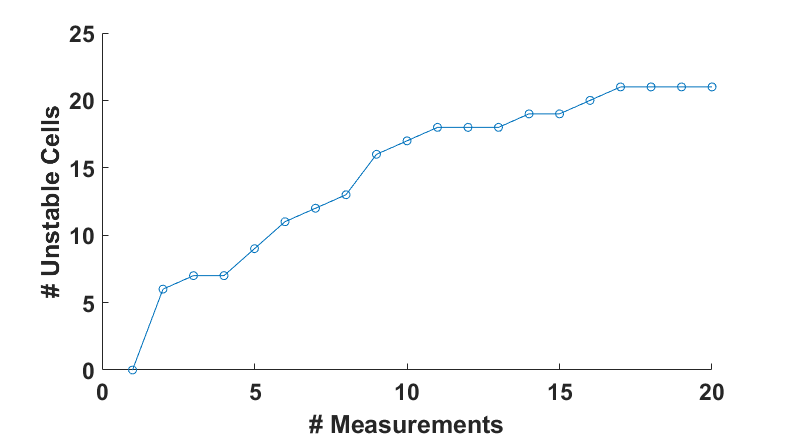
\includegraphics[width=14cm]{images/MEunstable_progression.png}
    \caption{Number of unstable SRAM cells with respect to the number of power-ups.}
    \label{fig:MEunstable_progression}
\end{figure}




\begin{figure}[H]
    \centering
    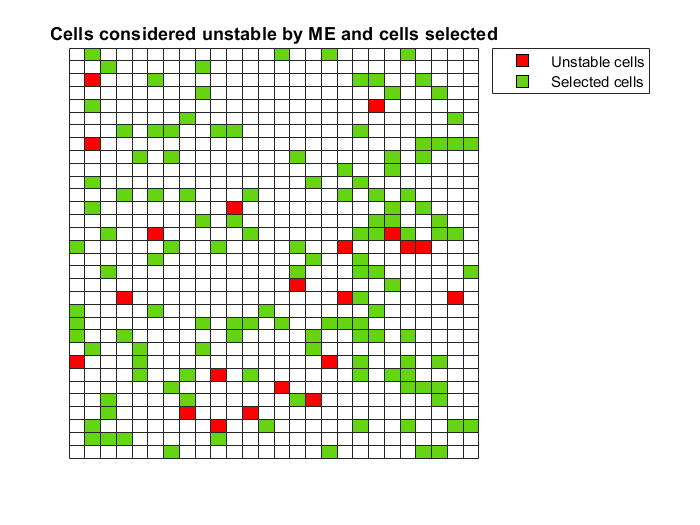
\includegraphics[width=14cm]{images/MEselection.png}
    \caption{Cell-wise representation of the bit selection performed through ME. Cells in red are those considered unstable and cells in green are those selected randomly among the rest.}
    \label{fig:MEselection}
\end{figure}

\subsection{Maximum trip supply voltage selection}

 MTSV selection is explored in detail in section \ref{sec:MTSV}. First, cells that are labelled as unstable due to random behavior during characterization are discarded. These cells are shown in red in fig. \ref{fig:unstable_all}. There are 48 in total, more than double compared to ME. Of the 21 cells labelled as unstable by ME, 17 are also labelled as unstable by MTSV (shown in black), i.e. 80\%. The 4 cells labelled as unstable by ME but not by MTSV (shown in blue) are assigned a low DRV value compared to the rest, so they will be considered weak cells and not form part of any reasonably sized selection. In this way, MTSV discards the cells that ME considers unstable and expands on that considerably.  
 
 \begin{figure}[H]
    \centering
    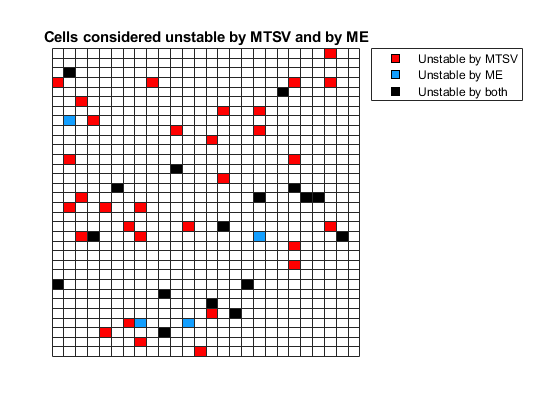
\includegraphics[width=14cm]{images/unstable_all.png}
    \caption{Cell-wise representation of the cells classified as unstable by ME or MTSV.}
    \label{fig:unstable_all}
\end{figure}
    


Then, cells are classified according to their DRV value. The 128 cells with the highest value are selected, which results in the selection \textit{MTSV Strongest}. Another possible scheme to have perfect uniformity is to select the 64 strongest cells biased to ``1'' and the 64 strongest cells biased to ``0'' since the preferred value of each cell is evaluated at enrollment. This selection is called \textit{MTSV Balanced}. The bits selected by either one are shown in fig \ref{fig:MTSVselection}. Cells in red are those considered unstable, cells in blue correspond to \textit{MTSV Strongest}, cells in purple to \textit{MTSV Balanced} and cells in green to both selection. The selections are very similar, differing only in about 10\% of cells. 

\begin{figure}[H]
    \centering
    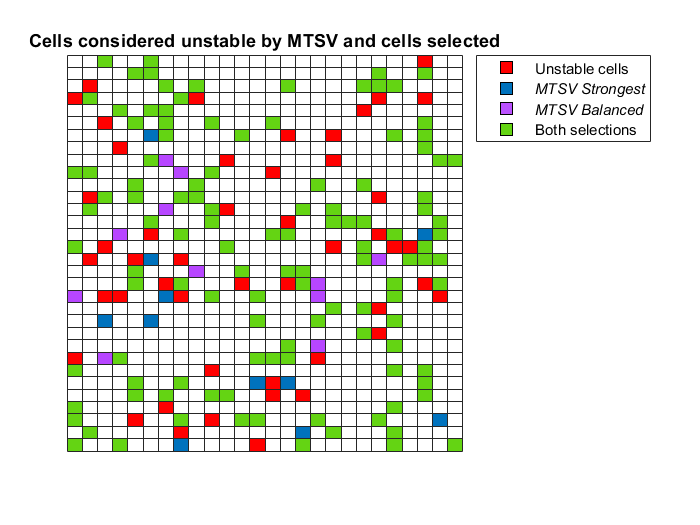
\includegraphics[width=14cm]{images/MTSVselection.png}
    \caption{Cell-wise representation of the bit selection performed through MTSV.}
    \label{fig:MTSVselection}
\end{figure}







\section{Nominal conditions}

Nominal conditions mean room temperature around $\SI{25}{\degree C}$ and a supply voltage of $\SI{1.2}{V}$. Multiple tests with a varying number of power ups for all cells were performed. The results can be found in Table \ref{tab:Nom}. BER and MAXintraHD are calculated intrinsically, i.e. using each dataset as its own reference. 

% in the range of $\SI{22}{\degree C}$ to $\SI{27}{\degree C}$

\begin{table}[H]
  \centering
  \caption{Performance of all cells under nominal conditions.}
    \begin{tabular}{|c|c|c|c|}
    \hline
    Measurements & BER(\%)   & MAXintraHD(\%) & Hamming Weight(\%) \bigstrut\\
    \hline
    200   & 0.4140 & 1.0830 & 50.83 \bigstrut\\
    \hline
    200   & 0.5102 & 1.0830 & 50.94 \bigstrut\\
    \hline
    200   & 0.4693 & 1.2034 & 50.84 \bigstrut\\
    \hline
    1000  & 0.4716 & 1.0830 & 50.94 \bigstrut\\
    \hline
    2000  & 0.5221 & 1.4440 & 51.03 \bigstrut\\
    \hline
    \end{tabular}%
  \label{tab:Nom}%
\end{table}%

BER varies between a value of 0.4140\% and 0.5221\%. This is for multiple tests and stays in a reduced bracket of values for a statistical metric. These values for nominal conditions are considerably low compared to other SRAM PUFs. In \cite{Schrijen2012}, seven different commercial and research SRAM designs are tested under nominal conditions as well as temperature and supply voltage variations.  BER values go between 2.8\% and 4.8\% for nominal conditions in these tests. However, our results are still far away from the desired reliability.

Maximum intra hamming distance is low, with the highest value obtained for the 2000 measurements of 1.444 \%. Hamming weight indicates a very slight bias towards one (Values between 50.83 \% and 51.03 \%), which is an acceptable range. Since the 2000 measurements are the most complete set they will be the ones used from this point onwards as measurements under nominal conditions and to obtain the chip's golden response. One interesting representation is the distribution of BER across the array to see if it follows any spatial pattern. This is shown in fig. \ref{fig:BER_2000_Nom}, and there is no noticeable pattern. It seems clear that most of the errors come from a few cells. Another useful cell-wise representation shown in fig. \ref{fig:p_2000_Nom} is the probability of each cell to power-up as either ``1'' or ``0'', obtained from the approximation of eq. \ref{eq:prob}.


 \begin{figure}[H]
    \centering
    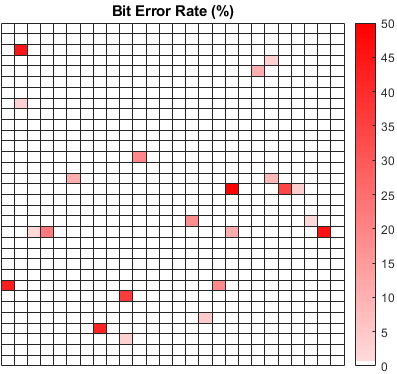
\includegraphics[width=7cm]{images/BER_2000_Nom.png}
    \caption{Cell-wise  representation of BER for the 2000 measurements under nominal conditions. }
    \label{fig:BER_2000_Nom}
 \end{figure}

% Most of the cells with a noticeable BER in fig. \ref{fig:BER_2000_Nom} are labelled as unstable. Cells with a BER of 0 \% under nominal condition are too. This may seem contradictory, but it is important to consider that cells that may appear stable under nominal conditions can be unstable under worse conditions. 



\begin{figure}[H]
    \centering
    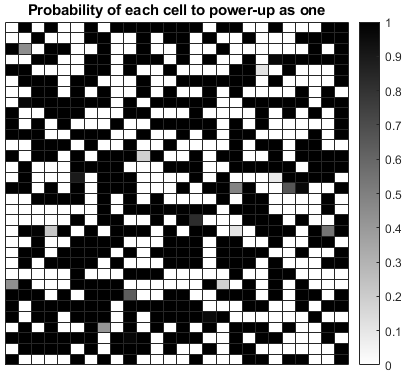
\includegraphics[width=7cm]{images/p_2000_Nom.png}
    \caption{Probability of each cell to power up as ``1'' based on 2000 measurements under nominal conditions. }
    \label{fig:p_2000_Nom}
\end{figure}

Again, no spatial pattern is observed and the distribution of values appears random.  

The performance of the selections presented before under nominal conditions is now examined. BER, maximum intra hamming distance and hamming weight are considered in Table \ref{tab:nom_selections}.

\begin{table}[H]
  \centering
  \caption{Performance of different selections of 128 bits when performing 2000 power-ups under nominal conditions.}
    \begin{tabular}{|c|c|c|c|}
    \hline
    Selection& BER(\%)   & MAXintraHD(\%) & Hamming Weight(\%) \bigstrut\\
    \hline
   \textit{First}& 0.4625 & 2.3438 & 48.07 \bigstrut\\
    \hline
    \textit{Random} & 0.6398 & 3.1250 & 45.11 \bigstrut\\
    \hline
    \textit{ME Stable} & 0.0227 & 0.7813 & 52.32 \bigstrut\\
    \hline
    \textit{MTSV Strongest} & 0.0012 & 0.7813 & 41.41 \bigstrut\\
    \hline
    \textit{MTSV Balanced} & 0.0012 & 0.7813 & 50 \bigstrut\\
    \hline
    \end{tabular}%
  \label{tab:nom_selections}%
\end{table}%

As expected \textit{First} and \textit{Random} have BER values similar to the ones shown in Table \ref{tab:Nom}. Their maximum intra hamming distance is higher due to taking a smaller sample size. \textit{ME Stable} shows a substantial improvement over the values shown in Table \ref{tab:Nom}. BER has reduced from around 0.4-0.6 \% to 0.0227 \%. Hamming weight indicates a result close to uniform, with 52.32 \%. For \textit{MTSV Strongest} and \textit{MTSV Balanced}, BER is reduced even more, going as low as 0.0012 \%. This is one order of magnitude better than \textit{ME Stable}, proving the advantages of the proposed method. 

It is important to keep this very small value for BER in perspective. 2000 power-ups per cell amount to $\SI{2.56}{\cdot 10^5}$ total power-ups for 128 cells. According to eq. \ref{eq:BER}, there were 3 total erroneous power-ups out of  $\SI{2.56}{\cdot 10^5}$. However, these BER values are still not good enough to meet the target of $\SI{7.8}{\cdot 10^{-7}\ \%}$.

Regarding uniformity, there is a significant bias in favor of cells that have ``0'' as a preferred value for \textit{MTSV Strongest}. A hamming weight of around 41 \% is 10\% lower than the hamming weight for all cells. This could be due to the cells' layout, although it is fully symmetric. At this moment, this is an open topic that needs investigation. Further experiments and research are being performed to explain this difference. 

\textit{MTSV Balanced} solves this issue, which is important to avoid leakage of information by the helper data. Hamming weight naturally indicates perfect uniformity at 50 \%. BER is the same as with \textit{MTSV Strongest}, so taking this selection would not come at a significant cost in reliability, at least under nominal conditions. 


\section{Environmental variations}

For measurements under environmental variations, only BER is considered since it is the most relevant metric for reliability.  200 power-ups were performed for each cell at each environmental condition. This is significantly lower than the 2,500 performed in the last chapter due to the fact that 832 cells are evaluated in each case, not just 100. 

\subsection{Resilience to supply voltage variations}

In this set of measurements, cells were powered up 200 times at room temperature and different supply voltages, i.e., raising their supply voltage from ground (\SI{0}{V}) to \SI{1.08}{V}, \SI{1.14}{V}, \SI{1.26}{V} and \SI{1.32}{V}. This corresponds to a range of the nominal voltage $1.2 \ \mathrm{V} \pm 10\%$. 

\begin{table}[H]
  \centering
  \caption{Mean BER value for the different selections when performing 200 power-ups under supply voltage variations}
    \resizebox{\linewidth}{!}{%
    \begin{tabular}{|c|c|c|c|c|c|c|}
    \hline
    $V_{DD}$ (V)   & All  & \textit{First} & \textit{Random} & \textit{ME stable} & \textit{MTSV Strongest} & \textit{MTSV Balanced} \bigstrut\\
\hline
1.08   & 0.5355 & 0.3164 & 0.9492 & 0.1172 & 0.0078 & 0.0078 \bigstrut\\
\hline
1.14   & 0.5788 & 0.4023 & 1.0469 & 0.1406 & 0     & 0 \bigstrut\\
\hline
1.26   & 0.6444 & 0.3555 & 1.0117 & 0.043 & 0     & 0 \bigstrut\\
\hline
1.32   & 0.7148 & 0.375 & 1.0508 & 0.0391 & 0.0039 & 0.0039 \bigstrut\\
\hline
\end{tabular}%
}
  \label{tab:vdd_sel}%
\end{table}%

BER increases slightly as $V_{DD}$ increases according to this data. The change in reliability is not very significant, as expected. The worst BER is obtained for a supply voltage of \SI{1.32}{V}. Bit selection techniques show a similar improvement to the one done under nominal conditions. \textit{MTSV Strongest} and \textit{MTSV Balanced} show low errors so these selections are robust under supply voltage variations. 



\subsection{Resilience to temperature variations}

% Table generated by Excel2LaTeX from sheet 'General analysis'
\begin{table}[b]
\small
  \centering
  \caption{Mean BER value for the different selections when performing 200 power-ups under temperature variations}
  \resizebox{\linewidth}{!}{%
    \begin{tabular}{|c|c|c|c|c|c|c|}
    \hline
    T (°C) & All & \textit{First} & \textit{Random} & \textit{ME stable} & \textit{MTSV Strongest} & \textit{MTSV Balanced} \bigstrut\\
    % Table generated by Excel2LaTeX from sheet 'General analysis'
\hline
-20  & 2.4272 & 2.2578 & 1.6641 & 0.0117 & 0.039 & 0.0039 \bigstrut\\
\hline
0    & 1.3267 & 0.8125 & 0.9844 & 0     & 0     & 0 \bigstrut\\
\hline
10   & 0.9344 & 0.5234 & 0.9844 & 0.0078 & 0     & 0 \bigstrut\\
\hline
20   & 0.8057 & 0.3789 & 0.9766 & 0.0195 & 0     & 0 \bigstrut\\
\hline
40   & 0.9615 & 0.7656 & 1.2734 & 0.3711 & 0     & 0 \bigstrut\\
\hline
\end{tabular}%
}
  \label{tab:temp_sel}%
\end{table}%

In these tests, instead of using the ACS climatic chamber employed in the previous chapter, a Thermonics T-2650BV is used. It allows for a larger range of temperatures by setting a determined temperature for the IC chip without affecting the whole PCB. 200 power-ups were performed for each cell, at $\SI{-20}{\degree C}$, $\SI{0}{\degree C}$, $\SI{10}{\degree C}$, $\SI{20}{\degree C}$ and $\SI{40}{\degree C}$. The resulting BER is shown in Table \ref{tab:temp_sel}. Measurements at higher temperature were attempted, but the results did not agree with the expected value found in literature and simulations. More experiments were planned, but the Thermonic T-2650BV broke down, and they could not be performed.





The changes in BER due to temperature variations are more noticeable. As temperature deviates from $\SI{20}{\degree C}$ upwards or downwards, BER increases. From $\SI{-20}{\degree C}$ to $\SI{40}{\degree C}$,  \textit{MTSV Strongest} and \textit{MTSV Balanced} selections are able to provide  practically error free results. 

% However, for $\SI{60}{\degree C}$ and specially $\SI{80}{\degree C}$ BER becomes too high and ME or MTSV bit selection does not seem to improve reliability significantly. This is because at these temperatures all cells biased to ``0'' present at least one bitflip, i.e. they are biased to be more unstable, while cells biased to ``1'' remain mostly stable. This is clearly shown in figure \ref{fig:p_200_80C}, where there are no cells in white. 

% \begin{figure}[H]
%     \centering
%     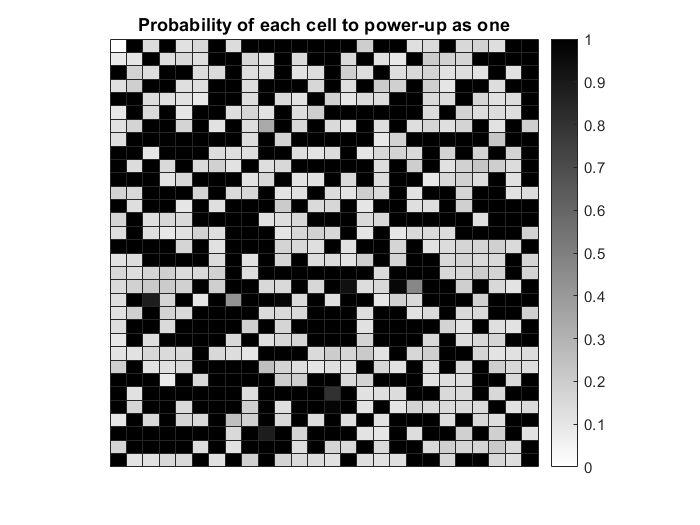
\includegraphics[width=13cm]{images/p_200_80C.png}
%     \caption{Probability of each cell to power-up as ``1'' based on 200 measurements at $\SI{80}{\degree C}$.}
%     \label{fig:p_200_80C}
% \end{figure}

% The cell-wise BER for the 200 measurements at $\SI{80}{\degree C}$ is represented in fig. \ref{fig:BER_80C}. A general increase of the BER value in the array is observed, although some cells considered unstable at room temperature are now more stable. Actually, both behaviours (increase and decrease of stability with temperature) have been confirmed through simulation and depend on the mismatch of the PMOS and NMOS transistors of the cell. In the literature there are reported studies that confirm a similar degradation of the BER values with temperature \cite{Schrijen2012}, with average BERs for different devices going from 6.6\% to 10.5\% for $\SI{80}{\degree C}$, although proportionally the increase is much smaller.

% \begin{figure}[H]
%     \centering
%     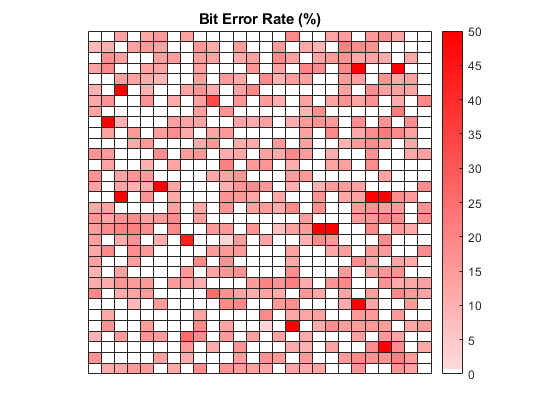
\includegraphics[width=12cm]{images/BER_80_C.png}
%     \caption{Cell-wise representation of BER for 200 measurements at $\SI{80}{\degree C}$. }
%     \label{fig:BER_80C}
% \end{figure}


% Evaluating the hamming weight of all cells at different temperatures the decrease in reliability of cells biased to ``0'' can be quantified. At $\SI{40}{\degree C}$, hamming weight is 50.51 \%, close to uniform. However, at  $\SI{60}{\degree C}$ it increases to 51.56 \% and at  $\SI{80}{\degree C}$ it goes up to 57.58 \%. In \cite{Schrijen2012}, changes in hamming weight with temperature are in the order of 1\%, not 7\%. The reason for such a heavy reduction in reliability only for cells biased to ``0'' is unclear, and is presently under study. In principle, the design of SRAM cells is symmetrical so there should not be such a considerable difference between the behaviour of cells biased to ``1'' or ``0''. Measurements performed after this test under nominal conditions show no increase in BER, so there was no permanent damage caused by the high temperature.  
% If this increase was normal, no selection should be able to significantly reduce the BER, which is incoherent with works such as \cite{Liu2017} where the BER is reduced down to 0 \% through a data remanence bit selection technique even for measurements at $80 \degree$C. 

% Observing these results, an attempt to repeat the same experiments on more samples was performed, so that this behaviour could be confirmed. Unfortunately, the thermal equipment used for them (Thermonics T-2650BV) was experiencing working problems during the last months, and definitely broke down just after measurements on chip \#6 were done. Further studies will be performed in the next months when new equipment will be available.  



\subsection{Resilience to circuit aging}

In this section, the procedure described in section \ref{ss:aging} is employed to evaluate the adequacy of the selections for cells under accelerated aging. In this case, all the cells were stressed. The measures performed are right after stress ended, 8 days later and 21 days later. It is important to point out that measurements right after stress are not instantaneous, it takes about 100 seconds to perform the 200 power-ups. The BER for each selection and point in time $t$ are shown in Table \ref{tab:aging_sel}.

\begin{table}[H]
\resizebox{\linewidth}{!}{%
\begin{tabular}{|c|c|c|c|c|c|c|}
\hline
    $t$ & All & \textit{First} & \textit{Random} & \textit{ME stable} & \textit{MTSV Strongest} & \textit{MTSV Balanced} \bigstrut\\
\hline
Before & 0.7858 & 0.6836 & 1.4453 & 0.043 & 0     & 0 \bigstrut\\
\hline
Right after stress & 7.4049 & 6.9492 & 6.4297 & 4.6523 & 1.0586 & 0.8477 \bigstrut\\
\hline
8 Days & 4.7918 & 5.8438 & 4.6914 & 1.9297 & 0.0039 & 0.0039 \bigstrut\\
\hline
21 Days & 4.7136 & 5.1406 & 4.6719 & 1.2227 & 0 & 0 \bigstrut\\
\hline
\end{tabular}%
}
  \caption{Mean BER value for the different selections when performing 200 power-ups at different points in time after accelerated aging.}
  \label{tab:aging_sel}%
\end{table}%

 \vspace*{-\baselineskip}


\begin{figure}[b!]
    \centering
    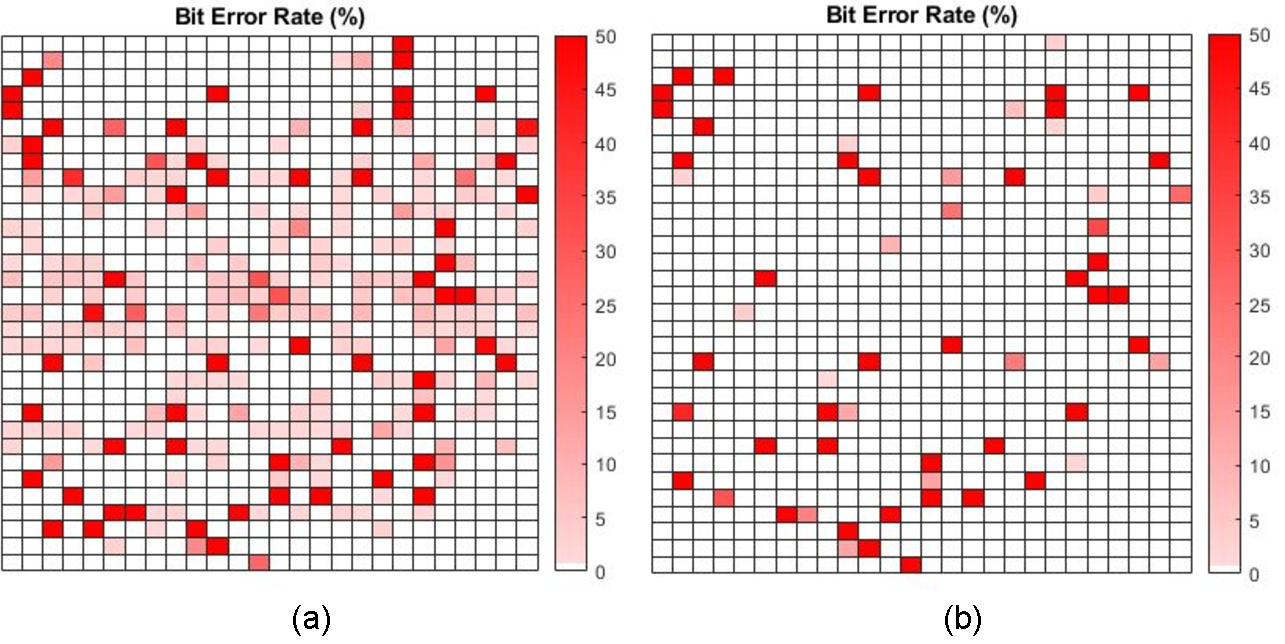
\includegraphics[width=14cm]{images/BER aging comparison.pdf}
    \caption{Cell-wise representation of BER for 200 measurements right after stress (a) and 8 days later (b). }
    \label{fig:BER_aging_comparison}
\end{figure}

The degradation of the cells is quite clear, with BER being around 10 times larger before and after stress for all cells (from 0.7858 \% to 7.4049 \%). \textit{First} and \textit{Random} have values close to \textit{All cells}, as expected. The temporal component of BTI is demonstrated by the decrease of about 3 \% in BER for all cells after 8 days. A measurement 21 days later shows some recovery, but it is considerably smaller. The recovery can be observed graphically by comparing the cell-wise BER right after stress, as shown in fig. \ref{fig:BER_aging_comparison} (a) and 8 days later, as shown in fig. \ref{fig:BER_aging_comparison} (b).  

\textit{ME stable} is capable of reducing the BER by about 3\%, but these values are still high. The results for either MTSV selection are outstanding. Right after stress BER is reduced to 1.0586 \% for \textit{MTSV Strongest} and to 0.8477 \% \textit{MTSV Balanced}. After 8 days it goes down to 0.0039 \% for both of them, and after 21 the selected cells achieve 0\% BER, the value obtained before stress. It clearly shows how MTSV is able to select those cells resilient to aging while the ME technique cannot. 





\section{Complete cryptographic solution}

Once the PUF response has been fully characterized, a complete HDA scheme can be implemented with these measurements. The fuzzy commitment construction explained in section \ref{sec:HDAs} will be employed, where a secret key is obfuscated through the PUF response. To measure the validity of this construction, each time the key is recovered successfully, it will be counted as a success. The Acceptance Rate (AR) will be the number of successful recoveries. In this way, it can range from zero, for no successful recoveries, to the number of attempts, where the key is successfully recovered each time. 

As discussed in chapter \ref{ss:ecc}, there are plenty of choices available as an ECC. Considering the low BER for both MTSV selections, a repetition code seems like the best choice. This code is the simplest to implement, essential for resource-constrained devices, has good error correction capabilities and will not require many bits since BER is already significantly reduced by the selection. To generate a 128-bit key, only two repetition codes use less than 832 bits: $R[3,1,3]$, which uses 384 bits and $R[5,1,5]$, which uses 640. Naturally, new selections are required for these sizes, performed by following the same criteria explained earlier. As MTSV classifies cells according to their strength, a larger selection will have higher BER.   

First, the HDA will be implemented with the power-ups performed under nominal conditions for the different selections. Then, it should be tested in a bad corner for reliability. The measurement right after accelerated aging is not considered, as applying such a high stress for an extended period of time is not realistic in actual implementations. A better approach is to use the measurements at low temperature, $-20 \degree$C, as well as those taken 8 days after accelerated aging, as they have a considerable increase in BER and can be trusted to represent a realistic degradation of reliability. 

Afterwards, one interesting test is to try and recover the key with a response from another chip. There should be an AR of zero, as each PUF is unique. Finally, the theoretical requirements of the repetition code for each scenario based on the BER measurements are examined. 



\subsection{Key generation under nominal conditions}

First, the 2000 power-ups performed under nominal conditions are used to test this construction. The helper data corresponding to each selection and repetition code is generated once (Enrollment) and each one of the 2000 power-ups are employed as individual attempts to recover the key (Reconstruction). The helper data generated during enrollment will be the one used in the other tests.

Results regarding AR are shown in Table \ref{tab:AR_nominal}, where $n$ refers to the parameter of the repetition code. The AR is high for all selections, but it is expected as the number of measurements is low for a BER of around 0.5 \%. In any case, for $R[3,1,3]$, \textit{First} shows one error and \textit{Random} seven. These errors no longer occur if the repetition code is expanded to $R[5,1,5]$, showing how a code with more redundancy has higher error correcting capabilities.   
% To illustrate this procedure with real data, the variables used during the enrollment phase and one reconstruction are shown for the \textit{First} selection and $R[3,1,3]$.

% During enrollment, the PUF response used to obfuscate the data is generated:

% \longstring{1,0,1,0,0,1,0,1,1,1,1,1,1,1,0,1,1,0,0,1,0,0,0,1,1,0,0,1,0,0,0,1,1,0,0,1,0,1,1,0,1,0,0,1,0,0,0,1,1,1,1,1,0,0,1,1,0,0,1,0,0,1,0,0,1,0,0,1,0,0,0,0,0,0,1,0,1,0,0,1,1,0,0,1,1,0,1,1,1,0,1,0,1,0,0,1,0,1,1,1,1,1,1,1,1,0,0,0,0,1,1,0,1,0,0,1,0,0,0,0,1,1,0,0,1,0,0,0,1,0,1,1,1,0,1,1,0,0,0,1,0,0,1,1,1,1,1,1,0,1,0,0,0,0,1,0,0,1,1,0,1,0,1,0,0,1,0,1,0,0,1,0,1,0,0,0,0,1,0,1,0,0,1,1,1,1,1,1,1,0,1,0,1,1,1,1,1,0,0,1,1,1,1,1,0,1,1,1,0,0,1,1,1,0,0,0,1,1,0,0,0,1,0,0,0,0,1,0,1,0,1,0,1,1,0,1,0,1,0,0,0,1,0,0,1,1,1,1,1,0,1,0,1,0,0,0,0,0,1,1,1,1,0,0,1,1,1,0,0,1,0,0,1,0,1,0,1,1,0,0,0,0,1,0,1,0,0,1,1,1,0,1,0,0,1,0,0,1,0,0,0,0,1,0,1,1,0,1,1,0,0,1,0,1,1,0,1,0,1,1,1,0,1,0,0,1,0,1,1,0,0,1,0,1,1,1,1,0,1,0,0,0,1,1,1,1,0,0,0,1,1,1,0,0,1,1,1,1,1,0,1,1,1,0,1,0,0,0,0,0,1,1,1,0,0,0,0,1,0,1,0,0,0,0
% }

\begin{table}[H]
\resizebox{\linewidth}{!}{%
\begin{tabular}{|c|c|c|c|c|c|c|c|c|c|c|}
\hline
 & \multicolumn{2}{c|}{\textit{First}} & \multicolumn{2}{c|}{\textit{Random}} & \multicolumn{2}{c|}{\textit{ME stable}} & \multicolumn{2}{c|}{\textit{MTSV Strongest}} & \multicolumn{2}{c|}{\textit{MTSV Balanced}} \bigstrut\\
\hline
$n$     & 3 & 5 & 3 & 5 & 3 & 5 &  \ \ \ \  3  \ \ \ \  & 5 &  \ \ \ \  3  \ \ \ \ & 5 \bigstrut\\
\hline

Required bits     & 384 & 640 & 384 & 640 & 384 & 640 &  384 & 640 &  384 & 640 \bigstrut\\
\hline
BER (\%)  & 0.2622 & 0.5447 & 0.6023 & 0.4178 & 0.0164 & 0.0133 & 0.0007 & 0.0016 & 0.0007 & 0.0016 \bigstrut\\
\hline
AR    & 1999 & 2000 & 1993 & 2000 & 2000 & 2000 & 2000 & 2000 & 2000 & 2000 \bigstrut\\
\hline
\end{tabular}%
}
  \caption{BER and AR value for the different selections when performing 2000 power-ups under nominal conditions using two different repetition codes.}
  \label{tab:AR_nominal}%
\end{table}%

\subsection{Key generation at low temperature}

 For $\SI{-20}{\degree C}$ less power-ups were performed, 200, so the AR will go up to that value. Results are shown in Table \ref{tab:AR_-20C}. There are more erroneous responses this time, specially considering how the number of power-ups is 10 times lower. It is clear how the decrease in reliability, i.e. the increase in BER, translates into a decrease in AR, and why considering only measurements under nominal conditions is not enough. Only \textit{MTSV Balanced} is able to recover the key 200 times for $R[3,1,3]$. There is one specific power-up with a larger number of bit-flips, due to the statistic nature of this process. This power-up is enough to cause one error in most selections. Even after applying a $R[5,1,5]$ only the selections based on MTSV are able to recover the key, showing once again its advantages versus multiple evaluation. 


\begin{table}[H]
\resizebox{\linewidth}{!}{%
\begin{tabular}{|c|c|c|c|c|c|c|c|c|c|c|}
\hline
 & \multicolumn{2}{c|}{\textit{First}} & \multicolumn{2}{c|}{\textit{Random}} & \multicolumn{2}{c|}{\textit{ME stable}} & \multicolumn{2}{c|}{\textit{MTSV Strongest}} & \multicolumn{2}{c|}{\textit{MTSV Balanced}} \bigstrut\\
\hline
$n$     & 3     & 5     & 3     & 5     & 3     & 5     & \ \ \ \  3  \ \ \ \  & 5 &  \ \ \ \  3  \ \ \ \     & 5 \bigstrut\\
\hline
Required bits     & 384 & 640 & 384 & 640 & 384 & 640 &  384 & 640 &  384 & 640 \bigstrut\\
\hline
BER (\%)   & 1.5299 & 2.1696 & 3.4792 & 2.1273 & 0.7643 & 1.4500  & 0.0143 & 0.2203 & 0.0938 & 0.2453 \bigstrut\\
\hline
AR    & 198  & 199  & 60  & 199  & 199  & 199 & 199  & 200  & 200  & 200 \bigstrut\\
\hline
\end{tabular}%
}
  \caption{BER and AR value for the different selections when performing 200 power-ups at $\SI{-20}{\degree C}$ using two different repetition codes.}
  \label{tab:AR_-20C}%
\end{table}%

\subsection{Key generation after accelerated aging}

As in the previous test, 200 power-ups are employed. The AR obtained for each selection and repetition code is shown in Table \ref{tab:AR_aging}. In this case, except for \textit{First} and \textit{Random} for a repetition code $R[3,1,3]$, the key is recovered successfully each time. This may seem counter-intuitive considering how AR was lower in the previous test while BER is higher in this one. However, it is explained by considering that the way BER is distributed matters greatly for key generation. In the previous test, there was one power-up that showed more bit-flips. Out of 200 power-ups, it does not have a large impact in the average BER, but it does translate in one failure to recover the key. 

\begin{table}[H]
\resizebox{\linewidth}{!}{%
\begin{tabular}{|c|c|c|c|c|c|c|c|c|c|c|}
\hline
 & \multicolumn{2}{c|}{\textit{First}} & \multicolumn{2}{c|}{\textit{Random}} & \multicolumn{2}{c|}{\textit{ME stable}} & \multicolumn{2}{c|}{\textit{MTSV Strongest}} & \multicolumn{2}{c|}{\textit{MTSV Balanced}} \bigstrut\\
\hline
$n$  & 3     & 5     & 3     & 5     & 3     & 5     & 3     & 5     & 3     & 5 \bigstrut\\
\hline
Required bits     & 384 & 640 & 384 & 640 & 384 & 640 &  384 & 640 &  384 & 640 \bigstrut\\
\hline
BER (\%)   & 4.4766 & 4.5484 & 5.4375 & 4.7492 & 2.8672 & 3.7188 & 0.0482 & 1.0211 & 0.0482 & 0.9695 \bigstrut\\
\hline
AR    & 186   & 200     & 139   & 200     & 200     & 200     & 200     & 200     & 200     & 200 \bigstrut\\
\hline
\end{tabular}%
}
  \caption{BER and AR value for the different selections when performing 200 power-ups 8 days after accelerated aging using two different repetition codes.}
  \label{tab:AR_aging}%
\end{table}%

\subsection{Key generation using other chips}

In this test, an attempt to recover the key with a different chip is performed. To do this, the helper data generated under nominal conditions for this chip is used in combination with the 200 power-ups measured for each of the five chips employed in the previous chapter, resulting in 1000 power-ups to work with. For any selection or repetition code, the AR obtained is 0, showing that a chip cannot be used to recover the key obfuscated by another chip. This verifies the uniqueness of the PUF, although on a small scale since only 6 chips are used in total.


\subsection{Repetition code requirements for low KER}

So far, different repetition codes have been tested with real measurements. However, the target for KER was set at $10^{-4}$ \%. It is important to remember that this means around one error per million attempts. In our measurements, the largest number of power-ups performed was 2000 under nominal conditions, and to verify that the KER target is met with statistical significance power-ups in the order of a million would be required at a bad corner of reliability, which is not feasible. 
Instead, the error reduction capabilities of the repetition code can be estimated using the binomial distribution (equation \ref{eq:binomialpmf}).  Since more than half of the bits need to fail, the probability of failure after the repetition code will be the cumulative probability $P\left(x\geq \frac{n+1}{2}\right)$ for $p=\mathrm{BER}$ and $R[n,1,n]$. This probability can be calculated through MATLAB, and the lowest $n$ that meets the requirements is chosen. To differentiate the two stages, $\mathrm{BER}_0$ is the BER before applying an ECC and $\mathrm{BER}_F$ the BER after ECC. As a reminder, the target $\mathrm{BER}_F$ is $\SI{7.8}{\cdot 10^{-7}\ \%}$ for a KER of $10^{-4} \%$. 

Leaving out the measurements performed right after applying stress and taking the values for 128-bit selections, the worst case for each selection is a BER of 5.8438 \% for \textit{First}, 4.6914 \% for \textit{Random} and 1.9297 \% for \textit{ME Stable}, where these three values were obtained in the aging test 8 days after accelerated aging and 0.0078 \% for both \textit{MTSV Strongest} and \textit{MTSV Balanced}, obtained in the supply voltage test for 1.08 V. Since both \textit{MTSV Strongest} and \textit{MTSV Balanced} have the same $\mathrm{BER}_0$, they will be simply referred as \textit{MTSV} from now on. The results of this procedure are shown in Table \ref{tab:rep}.

 
 
 
 \begin{table}[H]
\resizebox{\linewidth}{!}{%
\begin{tabular}{|c|c|c|c|c|c|}
\hline
    Selection & $\mathrm{BER}_0$ (\%) & $C$ & $\mathrm{BER}_F$ (\%)& KER (\%)& PUF bits \bigstrut\\
\hline
\textit{First} & 5.8438 & $R[21,1,21]$ & 5.53 E-7 & 7.07 E-5 & 2688      \bigstrut\\
\hline
\textit{Random} & 4.6914 & $R[19,1,19]$  & 3.22 E-7 & 4.13 E-5 & 2432  \bigstrut\\
\hline
\textit{ME Stable} & 1.9297 & $R[13,1,13]$ & 1.54 E-7 & 1.93 E-5 & 1644  \bigstrut\\
\hline
\textit{MTSV} & 0.0078 & $R[5,1,5]$  & 4.75 E-10 & 6.07 E-8 & 640  \bigstrut\\
\hline
\end{tabular}%
}
  \caption{Required repetition code to meet the KER target for each selection.}
  \label{tab:rep}%
\end{table}%

The predicted reduction in required redundant bits is made apparent with these results. \textit{First} and \textit{Random} require a large amount of redundant bits, 2688 and 2432 bits respectively. While for \textit{ME Stable} the required bits are reduced significantly, down to 1644, it is still a large number. The repetition code is perhaps not ideal for these selections, but as seen in Table \ref{tab:ECCs} there is a limit on how efficient the code may be with higher complexity. For \textit{MTSV}, a $R[5,1,5]$ code will achieve a KER of $\SI{6.07}{\cdot 10^{-8}\ \%}$, considerably lower than the rest. The required bits are significantly reduced. These results are consistent with the measurements at low temperature, where only a MTSV based selection with $R[5,1,5]$ is able to recover the key successfully each time. 
 
 
%  Based on the results, two scenarios are going to be considered: \textit{Optimistic} and \textit{Pessimistic}. According to \textit{Pessimistic}, the worst corner measured is the one used as reference for the KER, as the PUF is expected to have a good response under the complete range of possible environmental conditions. This would clearly be the measurement taken for $80 \degree C$, where BER goes from around $7\%$ to $10\%$. However, as explained before, this BER is very high due to the fact that every cell biased to zero becomes unstable, which is unexpected in SRAM PUF cells. If this is the case, no selection should be able to significantly reduce the BER, which is incoherent with works such as \cite{Liu2017} where the BER is reduced down to 0 \% through a data remanence bit selection technique even for measurements at $80 \degree$C. 

% The other possible scenario is \textit{Optimistic}. The results for $60 \degree$C and $80 \degree$C are not considered due to the massive drop in reliability for cells biased to ``0'' uncharacteristic of SRAM PUFs. For the aging test the measurements after 8 days are used as reference, since in real applications the PUF will not be powered on permanently and will have time to recover from BTI degradation. Leaving out these three measurements, the worst case for each selection is a BER of 5.8438 \% for \textit{First}, 4.6914 \% for \textit{Random} and 1.9297 \% for \textit{ME Stable}, where these three values were obtained in the aging test 8 days after accelerated aging and 0.0078 \% for both \textit{MTSV Strongest} and \textit{MTSV Balanced}, both obtained in the supply voltage test for 1.08 V. Since both \textit{MTSV Strongest} and \textit{MTSV Balanced} have the same $\mathrm{BER}_0$, they will be simply referred as \textit{MTSV} from now on.

% Out of these two possible scenarios \textit{Optimistic} is chosen, since it provides a fairer comparison between selections which is the objective of this work. Considering the results obtained here and those present in the bibliography \cite{Liu2017,Schrijen2012}, a MTSV selection is expected to perform in line with the rest of tests for high temperatures in chips with different design. This assertion would need to be verified and is part of possible future work. 














 
 
 
 

% \section{Measurements: results and discussion}
% All of these metrics are tested for a variety of PUF measurements datasets obtained from different KIPT chips \cite{kipt}. They were done to verify the validity of the Maximum Trip Supply Voltage (MTSV) technique \cite{mtsv}, explained in detail in the next subsection. It's goal is to classify cells regarding their stability to improve the PUF's reliability. KIPT is a chip designed in UMC 65-nm CMOS technology for the characterization of aging and RTN effects on IC circuit blocks. Among other elements it has an array of 832 SRAM cells used for PUF-related tests, the one of interest in this case. These measurements include raw power-up data as well as tests where different operating parameters are modified. The validity of the MTSV technique is confirmed first under nominal conditions and specially after temperature and supply voltage variations as well as forced aging.  The metrics are implemented in MATLAB. In eachTableof data $m$ is the number of power-ups per cell performed in each case. 

% \subsection{Nominal characterizations}
% In the first place the nominal characterizations are considered. In these the golden response is obtained intrinsically, since they are the fresh characterizations used later as reference. These can be observed in Table \ref{tab:nom}. Measurements have been performed on two different sets of cells:
% \begin{itemize}
%     \item All the 832 cells in the array (All)
%     \item 50 strongest and 50 weakest cells among those considered stable by Maximum Trip Supply Voltage (SnW)
% \end{itemize}

% MTSV works as follows: Suppose a cell has a certain preferred value. If the cell is storing its non-preferred value and the supply voltage is gradually reduced, there will be a point where the value will flip. Accordingly, the sooner it flips the stronger the bias to the preferred value. This can be used to have a direct measurement on how stable the cell is. Cells that flip more than once during the supply voltage variation are considered unstable and are discarded and the rest are ranked from strongest to weakest according to their MTSV. The traditional method to determine stability was simply multiple evaluation \cite{Baturone2015}, i.e. measuring the PUF multiple times under nominal conditions and keeping the cells that have the same outcome more consistently. 

% Regarding reliability, using MTSV to clasify cells consistently reduces BER and makes the minimum entropy closer to 0 for both strong and weak cells, indicating more stability. Values can be compared in Table \ref{tab:nom}. Maximum intra hamming distance tends to increase, with values being around 1-2 \% for the whole array of cells and 4-8\% for SnW cells. This metric depends on the length of the response and the difference in the probabilistic outliers. Accordingly, it could be that decrease in length has more weight than the reduction of outliers from the preselection, even if the overall BER is improved. However, the fact that many more powerups were performed for SnW (from 2500 to 3700) than for all cells (200 in all chips) is probably the reason for a higher intraHD. Many more pairs of responses are compared for SnW and outliers will be more frequent the higher the samples. Generally the classification between strongest and weakest cells seems to work properly, with BER, MAXintraHD and minimum entropy being lower which indicates more reliability. There is one exception with chip 1, where BER and entropy are slightly higher for the strongest cells. This could be a statistical outlier and be caused by the fact that all cells considered stable have high reliability. It has to be considered that MTSV shines versus Majority Vote when operating conditions change, not so much in nominal conditions. 

% Upon examination of the hamming weight, it is clear that cells biased to 0 tend to be more stable, while those considered weakest tend towards 1 in all chips. Exact values across chips vary in a wide range from 0,32 to 0,44 for the strongest cells and from 0,60 to 0,68. The strongest cells have a hamming weight far from the ideal 0,5, which means that uniformity could be a problem when using MTSV to classify cells. The origin of this correlation between bias to 0 and stability is uncertain. It could be inherent to this metric or caused by the chip's design. This method should be employed in other designs to investigate further. The values for all cells are acceptable, close to 0,5 but with sizeable variation. Some are lower than 0,5 but there seems to be a slight tendency towards cells biased to one. The sample size isn't big enough to affirm it. 



% \subsection{Performance tests}
% In the following tests metrics were determined extrinsically by comparing power-up values of the 50 Strongest and 50 Weakest cells according to MTSV to their corresponding golden responses generated from the nominal characterizations explained before. 
% \subsubsection{Temperature variations}
% The first test was performance under temperature variations for chip 8, in a range from $0\degree$ to $40\degree$. Results are shown in Table \ref{tab:Temp}. Weakest cells perform better under the standard condition of 20$\degree$ and worse for lower and specially higher temperatures, with lower reliability and uniformity. Strongest cells remain stable through the range of temperatures. 
% \subsubsection{\texorpdfstring{$V_{dd}$}{Vdd} variations}
% The second test was to observe the stability of the response to supply voltage variations. The nominal value of the supply voltage is 1,2 V. A generous margin is to estimate possible variations as 10\% of this value, i.e. from 1,08 V to 1,32 V. It would seem like a voltage below the nominal value doesn't have a noticeable effect on reliability as observed in Table \ref{tab:Vdd}. For values above it the weakest cells seem to perform worse while the strongest remain stable once again, validating the MTSV classification. Uniformity isn't affected in either weak or strong cells. 
% \newpage
% \subsubsection{Circuit aging}
% In the third test aging is evaluated. First, the preferred value is written and stored at a high supply voltage (2.5 V) for 10000 s. This reinforces the non-preferred value due to bias temperature instability (BTI) CITE PREVIOUS CHAPTER. This kind of degradation has a permanent and a temporal component. To test it, measurements were performed at different dates.

% Strongest cells are not noticeably affected by this stress  as seen in Table \ref{tab:evolution}. Weakest cells however turn very unstable. Their tendency  is to ``regenerate'' themselves with time due to the temporal component of the degradation wearing off. In terms of uniformity the hamming weight of the weakest cells increases with stress but interestingly enough it increases even more as time goes by. 
% \subsection{Strongest 256 bits implementation}

% In real application scenarios nowadays cryptographic keys usually have 256 bits. An array with many times more cells than KIPT would be employed and the selection of 256 cells would represent a smaller percentage of the total cells. Accordingly, results should be better since there would be a higher number of cells from which to pick the best ones. It is interesting anyways to test how good this array would be when selecting the strongest 256 bits. Complete measurements of MTSV and all chips were performed for four chips, results of applying metrics to those can be found in Table \ref{tab:stable}. BER is still quite low and reliability is satisfactory and comparable to the previous measurement of the strongest 50 cells. Since more cells are selected uniformity improves, with a better hamming weight. It's closer to 0,5 but strong cells are still strongly biased to 0. 
% \subsection{Uniqueness}

% Since uniqueness is measured comparing responses across different chips, inter hamming distance values are separated from the rest and can be found in Table \ref{tab:inter}. The 256 strongest cells selection is used for the comparison because, as explained before, it emulates real application scenarios better. This means that only four chips are used which is a small sample size, so results are not definitive. To illustrate the hamming distance measurement process and since there are few possible pairs, the hamming distance between all pairs is shown. These values can be found in Table \ref{tab:inter}, and are averaged to obtain the inter hamming distance. Results for all cells are good, close to 50\% and with a clear tendency towards values lower than it. In the 256 cells, the result is a perfect 50\% for the mean. Examining each of the pairs, there is a sizeable variability in the HD of each pair going above and below 50\%. Such a good result is probably radom chance and a consequence of the small sample size, but it shows that in any case uniqueness should be within acceptable margins.  
% \newpage
% \subsection{True Random Number Generator}
% Lastly, the capability of the PUF to generate random numbers through the MTSV method is evaluated. In this case, the metric of most interest is entropy, the higher it is the better the result. It doesn't make sense to compare the metrics of a TRNG to an ideal string since the objective isn't to generate an unique identifier, so they are measured intrinsically. MTSV can be employed to create the TRNG as well. Suppose a cell is written with its non preferred value. Then, the voltage is decreased to the trip voltage of the cell, i.e., the voltage at which it flipped from its non-preferred to its preferred value at the MTSV procedure. Further measurements done at the trip voltage by this 
% method will be unpredictable since they are around the frontier between two outputs and a small variation can cause it to go one way or the other. The smaller the step is when determining this voltage the closer it will be to the actual frontier. Accordingly, the entropy and thus randomness will be higher which can be observed in Table \ref{tab:MTSV}. Reducing the step voltage would come at a cost in computation and hardware specifications. The results using all cells for this chip are included again in the last row for comparison. 

% Another method to have a TRNG using the MTSV would be to employ those cells that were discarded due to being unstable. This is similar to the method applied in \cite{Baturone2015}, where cells considered unstable through majority vote are used to generate random numbers. The result of employing cells considered unstable by MTSV is shown in Table \ref{tab:usntable}. The number of unstable cells $n$ is different in each case. The minimum entropy measured using those is considerable, ranging from 11\% to 22\% (High variability). This is comparable to using a step size of 2 mV in the previous case. The drawback is that the number of cells employed is much lower, whereas with the prior method all cells in the array are used. However, if a large number of cells are available in a bigger array, this method comes at no cost in computation or hardware specifications. Uniformity is important as well for a TRNG and the proposed MTSV method has better values, with a HW reasonably close to 0,5\% while using unstable cells leads to choosing cells biased strongly towards either 0 or 1.
% \newpage
% \subsection{Bias from MTSV and state-wise performance}

% The uniformity of the response can be checked with the hamming weight. In Table \ref{tab:256Strongest} bit error rate and hamming weight from 200 evaluations of the best 256 cells according to MTSV under nominal conditions are shown. The hamming weight has a clear tendency towards ``0'' in all chips. If MTSV works properly, this would indicate that cells biased to ``0'' are more stable since there are more of them among the selected 256 cells. 

% % Table generated by Excel2LaTeX from sheet 'Sheet1'
% \begin{table}[htbp]
%   \centering
%   \caption{Performance of the best 256 cells according to MTSV in different chips after 200 evaluations under nominal conditions.}
%     \begin{tabular}{|c|c|c|}
%     \hline
%     Chip  & BER   & Hamming Weight  \bigstrut\\
%     \hline
%     1     & 0.0020  & 45.71 \bigstrut\\
%     \hline
%     2     & 0.0098 & 44.54 \bigstrut\\
%     \hline
%     4     & 0.0039 & 43.75 \bigstrut\\
%     \hline
%     8     & 0.0020 & 42.58 \bigstrut\\
%     \hline
%     13    & 0.0039  & 41.80 \bigstrut\\
%     \hline
%     \end{tabular}%
%   \label{tab:256Strongest}%
% \end{table}%

% To verify the tendency, the performance of all stable cells according to MTSV biased to ``1'' (Table \ref{tab:ones}) is analyzed separately from the performance of those biased to ``0'' (Table \ref{tab:zeroes}). Mean MTSV is included. Each cell has associated a MTSV value obtained during characterization which is used to determine how biased it is and, accordingly, how stable it is. Mean MTSV is simply the mean of the values given to each cell. 

%  Cells biased to ``0'' have a higher mean MTSV than those biased to ``1'' in all chips. This explains why there are more cells biased to ``0'' among the 256 best cells according to MTSV. However, cells biased to ``0'' consistently perform worse in terms of BER than those biased to one by a decent margin. This is true across all chips. 

% Cells biased to ``0'' or ``1'' should have similar performance since both states are symmetric. Choosing which state is ``0'' and which state is ``1'' is arbitrary. If cells biased to ``1'' consistently outperform those biased to ``0'', it means that there was some asymmetry in the chip's design. One way to solve this problem is taking half of the cells biased to ``0'' and the other half to ``1'' for the response. It would guarantee perfect uniformity but would complicate the whole process as well. Another way to solve it is to use a chip where both types of cell perform equally. 

% However, the main issue is that MTSV gives cells biased to ``0'' a better ``score'' than those biased to ``1'' even if cells biased to ``1'' perform better. The cause for this error is harder to pinpoint, and the bias may be present regardless of the chip's design. A selection of best cells in a chip with a higher number of cells (instead of the 832 cells in ours) may end up only with cells biased to ``0'' if this tendency is present across designs. This would render the PUF useless. 
% \newpage


% % Table generated by Excel2LaTeX from sheet 'Sheet1'
% \begin{table}[htbp]
%   \centering
%   \caption{Performance of stable cells biased to zero after 200 evaluations in each chip}
%     \begin{tabular}{|c|c|c|c|}
%     \hline
%     Chip  & BER   & Mean MTSV & n \bigstrut\\
%     \hline
%     1     & 0.0078 & 0.1696 & 385 \bigstrut\\
%     \hline
%     2     & 0.0663 & 0.1675 & 362 \bigstrut\\
%     \hline
%     4     & 0.0493 & 0.171 & 355 \bigstrut\\
%     \hline
%     8     & 0.0639 & 0.1663 & 391 \bigstrut\\
%     \hline
%     13    & 0.0181 & 0.1664 & 387 \bigstrut\\
%     \hline
%     \end{tabular}%
%   \label{tab:zeroes}%
% \end{table}%


% % Table generated by Excel2LaTeX from sheet 'Sheet1'
% \begin{table}[htbp]
%   \centering
%   \caption{Performance of stable cells biased to one after 200 evaluations in each chip}
%     \begin{tabular}{|c|c|c|c|}
%     \hline
%     Chip  & BER   & Mean MTSV & n \bigstrut\\
%     \hline
%     1     & 0     & 0.1626 & 406 \bigstrut\\
%     \hline
%     2     & 0     & 0.1606 & 424 \bigstrut\\
%     \hline
%     4     & 0.0083 & 0.1624 & 424 \bigstrut\\
%     \hline
%     8     & 0     & 0.1581 & 387 \bigstrut\\
%     \hline
%     13    & 0.0063 & 0.1582 & 396 \bigstrut\\
%     \hline
%     \end{tabular}%
%   \label{tab:ones}%
% \end{table}%





% \chapter{Aging in the proposed error correction circuit}
% \input{chapters/chapter06}
\chapter{Conclusions}
In this work, a new bit selection technique (MTSV), an experimental procedure to evaluate the reliability of SRAM cells for their utilization in power-up PUFs, is exhaustively validated. First, by itself, showing its ability to distinguish unstable, strong and weak cells. Cells selected as strong are consistently shown to be considerably more reliable than those classified as weak under nominal conditions, temperature and supply variations and after accelerated aging. 

Afterwards, MTSV bit selection is tested in the context of using a SRAM PUF as a 128-bit key generator. This is done by comparing the performance of a selection based on MTSV with the performance of other possible selections. When measuring BER under nominal conditions, temperature and supply variations, as well as after accelerated aging, the MTSV-based selections consistently outperform the rest. Next, the ability of these selections to generate a key is tested by implementing a HDA based on the fuzzy commitment construction with a small repetition code. The results from this test demonstrate how MTSV-based selections are the only ones able to always recover the key successfully under different operating conditions. Finally, the required repetition code to achieve a KER lower than $10^{-4} \%$ for each selection is calculated. Although further measurements are still necessary to completely evaluate this method, specially at high temperatures, the results show quantitatively how much the requirements for the ECC are reduced, with a selection based on MTSV needing three to five times less redundant bits than the other selections. This considerably reduces the cost of implementation of SRAM PUFs, a matter of great importance due to their use in resource-constrained devices. The MTSV bit-selection technique represents one more step in the development of SRAM PUFs.

Future work will focus on implementing the MTSV technique in a commercial chip, including the enrollment and reconstruction phases, to demonstrate its capabilities in real implementations. Another step further would be to perform the hardware design to implement the complete crytographic solution on an IC, as well as evaluating the aging resilience of this design.



% \appendix
% \chapter*{Tables}
% 
% \begin{table}[htbp]
%   \centering
%     \caption{Nominal characterizations}
%     \vspace{5mm}
% % Table generated by Excel2LaTeX from sheet 'Sheet1'
% \begin{tabular}{|c|l|c|c|c|c|c|}

% \hline
% Chip & \multicolumn{1}{c|}{Type} & BER & MAXintraHD & HW & $H_{min}$ & Power-ups \bigstrut\\
% \hline
% \multirow{3}[6]{*}{1} & All & 0.3430 & 1.4440 & 51.57 & 0.5630 & 200 \bigstrut\\
% \cline{2-7}  & Strongest & 0.0064 & 4 & 36.01 & 0.0093 & 2800 \bigstrut\\
% \cline{2-7}  & Weakest & 0.0036 & 4 & 66.00 & 0.0052 & 2800 \bigstrut\\
% \hline
% \multirow{3}[6]{*}{2} & All & 0.7124 & 2.0457 & 53.08 & 1.2772 & 200 \bigstrut\\
% \cline{2-7}  & Strongest & 0.0040 & 4 & 40.00 & 0.0058 & 2500 \bigstrut\\
% \cline{2-7}  & Weakest & 0.1136 & 6 & 62.09 & 0.1675 & 2500 \bigstrut\\
% \hline
% \multirow{3}[6]{*}{4} & All & 0.5108 & 1.6847 & 53.42 & 0.8776 & 200 \bigstrut\\
% \cline{2-7}  & Strongest & 0.0016 & 4 & 44.00 & 0.0023 & 3700 \bigstrut\\
% \cline{2-7}  & Weakest & 0.0319 & 4 & 68.00 & 0.0462 & 3700 \bigstrut\\
% \hline
% 7 & All & 0.6394 & 2.0433 & 49.44 & 1.1051 & 200 \bigstrut\\
% \hline
% \multirow{3}[6]{*}{8} & All & 0.5397 & 1.8051 & 49.02 & 0.9119 & 200 \bigstrut\\
% \cline{2-7}  & Strongest & 0.0016 & 4 & 32.00 & 0.0023 & 2500 \bigstrut\\
% \cline{2-7}  & Weakest & 0.1568 & 6 & 60.15 & 0.2300 & 2500 \bigstrut\\
% \hline
% \multirow{2}[4]{*}{11} & Strongest & 0.0024 & 4 & 32.00 & 0.0035 & 2500 \bigstrut\\
% \cline{2-7}  & Weakest & 0.3752 & 8 & 60.19 & 0.5573 & 2500 \bigstrut\\
% \hline
% 12 & All & 0.5300 & 1.5644 & 51.30 & 0.9269 & 200 \bigstrut\\
% \hline
% \end{tabular}%



%   \label{tab:nom}%
% \end{table}%


% \begin{table}[htbp]
%   \centering
%   \caption{Peformance under temperature variations for chip 8. $m=2500$ and SnW selection}
%   \vspace{5mm}
% % Table generated by Excel2LaTeX from sheet 'Sheet1'
% \begin{tabular}{|c|l|c|c|c|c|}
% \hline
% Temperature & \multicolumn{1}{c|}{Type} & BER & MAXintraHD & HW & $H_{min}$ \bigstrut\\
% \hline
% \multirow{2}[4]{*}{0\degree} & Strongest & 0 & 0 & 32.00 & 0 \bigstrut\\
% \cline{2-6}  & Weakest & 1.7592 & 6 & 58.71 & 1.1365 \bigstrut\\
% \hline
% \multirow{2}[4]{*}{10\degree} & Strongest & 0.0024 & 2 & 32.00 & 0.0035 \bigstrut\\
% \cline{2-6}  & Weakest & 0.4080 & 4 & 59.88 & 0.6213 \bigstrut\\
% \hline
% \multirow{2}[4]{*}{20\degree} & Strongest & 0.0008 & 2 & 32.00 & 0.0012 \bigstrut\\
% \cline{2-6}  & Weakest & 0.1256 & 4 & 60.11 & 0.1846 \bigstrut\\
% \hline
% \multirow{2}[4]{*}{30\degree} & Strongest & 0.0024 & 2 & 32.00 & 0.0035 \bigstrut\\
% \cline{2-6}  & Weakest & 0.2288 & 4 & 60.23 & 0.3391 \bigstrut\\
% \hline
% \multirow{2}[4]{*}{40\degree} & Strongest & 0.0008 & 2 & 32.00 & 0.0012 \bigstrut\\
% \cline{2-6}  & Weakest & 1.2128 & 4 & 61.21 & 1.7592 \bigstrut\\
% \hline
% \end{tabular}%


%   \label{tab:Temp}%
% \end{table}%


% \begin{table}[htbp]
%   \centering
%   \caption{Peformance under $V_{dd}$ variations for chip 8. $m=2500$ and SnW selection}
%   \vspace{5mm}
% \begin{tabular}{|c|l|c|c|c|c|}
% \hline
% Vdd (mV) & \multicolumn{1}{c|}{Type} & BER & MAXintraHD & HW & $H_{min}$ \bigstrut\\
% \hline
% \multirow{2}[4]{*}{108} & Strongest & 0.0024 & 2 & 32.00 & 0.0035 \bigstrut\\
% \cline{2-6}  & Weakest & 0.1160 & 4 & 60.11 & 0.1707 \bigstrut\\
% \hline
% \multirow{2}[4]{*}{114} & Strongest & 0.0016 & 2 & 20.00 & 0.0023 \bigstrut\\
% \cline{2-6}  & Weakest & 0.1208 & 2 & 60.11 & 0.1773 \bigstrut\\
% \hline
% \multirow{2}[4]{*}{120} & Strongest & 0.0048 & 2 & 32.00 & 0.0069 \bigstrut\\
% \cline{2-6}  & Weakest & 0.1216 & 4 & 60.11 & 0.1783 \bigstrut\\
% \hline
% \multirow{2}[4]{*}{126} & Strongest & 0.0008 & 2 & 32.00 & 0.0012 \bigstrut\\
% \cline{2-6}  & Weakest & 0.1312 & 4 & 60.11 & 0.1922 \bigstrut\\
% \hline
% \multirow{2}[4]{*}{132} & Strongest & 0.0008 & 2 & 32.00 & 0.0012 \bigstrut\\
% \cline{2-6}  & Weakest & 0.2040 & 4 & 60.19 & 0.3027 \bigstrut\\
% \hline
% \end{tabular}%


%   \label{tab:Vdd}%
% \end{table}%

% \begin{table}[htbp]
%   \centering
%   \caption{Peformance evolution after applying a stress of 2.5 V for 10000 s  for chip 11. $m=2500$ and SnW selection}
%   \vspace{5mm}
% \begin{tabular}{|c|l|c|c|c|c|}
% \hline
% Date & \multicolumn{1}{c|}{Type} & BER & MAXintraHD & HW & $H_{min}$ \bigstrut\\
% \hline
% \multirow{2}[4]{*}{21-oct} & Strongest & 0 & 0 & 32.00 & 0 \bigstrut\\
% \cline{2-6}  & Weakest & 21.0424 & 26 & 70.96 & 2.3031 \bigstrut\\
% \hline
% \multirow{2}[4]{*}{29-oct} & Strongest & 0.0016 & 2 & 32.00 & 0.0023 \bigstrut\\
% \cline{2-6}  & Weakest & 19.2640 & 24 & 72.16 & 1.8278 \bigstrut\\
% \hline
% \multirow{2}[4]{*}{03-dic} & Strongest & 0.0008 & 2 & 32.00 & 0.0012 \bigstrut\\
% \cline{2-6}  & Weakest & 18.5720 & 28 & 73.22 & 7.2054 \bigstrut\\
% \hline
% \end{tabular}%


%   \label{tab:evolution}%
% \end{table}%
% % Table generated by Excel2LaTeX from sheet 'Sheet1'
% \begin{table}[htbp]
%   \centering
%   \caption{Performance for the strongest 256 bits. m=200}
%   \vspace{5mm}
%     \begin{tabular}{|c|c|c|c|c|}
%     \hline
%     Chip & BER & MAXintraHD & Hamming Weight & $H_{min}$ \bigstrut\\
%     \hline
%     1 & 0.002 & 0.3906 & 45.71 & 0.0028 \bigstrut\\
%     \hline
%     2 & 0.0098 & 0.3906 & 44.54 & 0.0141 \bigstrut\\
%     \hline
%     4 & 0.0039 & 0.3906 & 43.75 & 0.0056 \bigstrut\\
%     \hline
%     8 & 0.002 & 0.3906 & 42.58 & 0.0028 \bigstrut\\
%     \hline
%     \end{tabular}%
%   \label{tab:stable}%
% \end{table}%



% % Table generated by Excel2LaTeX from sheet 'Sheet1'
% \begin{table}[htbp]
%   \centering
%   \caption{Inter Hamming distance for all cells and the 256 strongest in chips 1. 2. 4 and 8. $m$=200}
%     \begin{tabular}{|c|c|c|}
%     \hline
%     Pairs & All & 256 Strongest \bigstrut\\
%     \hline
%     1/2 & 49.9398 & 51.9531 \bigstrut\\
%     \hline
%     1/3 & 46.5704 & 52.7344 \bigstrut\\
%     \hline
%     1/4 & 49.3381 & 46.8750 \bigstrut\\
%     \hline
%     2/3 & 49.0975 & 50.7813 \bigstrut\\
%     \hline
%     2/4 & 48.4958 & 47.2656 \bigstrut\\
%     \hline
%     3/4 & 49.9398 & 50.3906 \bigstrut\\
%     \hline
%     \hline
%     Mean & 48.8969 & 50.0000 \bigstrut\\
%     \hline
%     \end{tabular}%
%   \label{tab:inter}%
% \end{table}%

% \begin{table}[htbp]
%   \centering
%   \caption{TRNG employing MTSV with variable step sizes for chip 2 and $m=200$ }
%   \vspace{5mm}
%     % Table generated by Excel2LaTeX from sheet 'Sheet1'
% \begin{tabular}{|c|c|c|c|c|}
% \hline
% Step (mV) & BER & MAXintraHD & HW & $H_{min}$  \bigstrut\\
% \hline
% 50 & 1.316 & 3.2491 & 53.12 & 2.3182  \bigstrut\\
% \hline
% 20 & 1.801 & 4.3321 & 53.06 & 3.1214  \bigstrut\\
% \hline
% 10 & 3.105 & 6.4982 & 52.93 & 5.4470  \bigstrut\\
% \hline
% 5 & 4.961 & 10.5897 & 51.04 & 8.5994  \bigstrut\\
% \hline
% 2 & 9.678 & 19.2539 & 50.44 & 16.8163  \bigstrut\\
% \hline
% 1 & 12.136 & 21.6606 & 49.80 & 20.9342  \bigstrut\\
% \hline
% 0.5 & 13.732 & 23.9471 & 49.20 & 23.9649  \bigstrut\\
% \hline
% \hline
%     All cells &0.7124 & 2.0457 & 0.5308 & 1.2772 \bigstrut\\
%     \hline
% \end{tabular}%

%   \label{tab:MTSV}%
% \end{table}%
% % Table generated by Excel2LaTeX from sheet 'Sheet1'
% \begin{table}[htbp]
%   \centering
%   \caption{Performance for the unstable cells $m=200$}
%   \vspace{5mm}
%     \begin{tabular}{|c|c|c|c|c|c|}
%     \hline
%     Chip & n & BER & MAXintraHD & HW & $H_{min}$ \bigstrut\\
%     \hline
%     1 & 40 & 7.0500 & 17.5000 & 56.32 & 11.5885 \bigstrut\\
%     \hline
%     2 & 45 & 12.6222 & 24.4444 & 37.51 & 22.7909 \bigstrut\\
%     \hline
%     4 & 52 & 7.7596 & 15.3846 & 38.11 & 13.4027 \bigstrut\\
%     \hline
%     8 & 53 & 7.9906 & 18.8679 & 38.01 & 13.5867 \bigstrut\\
%     \hline
%     \end{tabular}%
%   \label{tab:usntable}%
% \end{table}%


\printbibliography{}

\clearpage



\clearpage

\end{document}